\documentclass[12pt,twoside,letterpaper]{article}

%%%%%%%%%%%%%%%%%%%%%%%%%%%%%%%%%%%%%%%%%
% University Assignment Title Page 
% LaTeX Template
% Version 1.0 (27/12/12)
%
% This template has been downloaded from:
% http://www.LaTeXTemplates.com
%
% Original author:
% WikiBooks (http://en.wikibooks.org/wiki/LaTeX/Title_Creation)
%
% License:
% CC BY-NC-SA 3.0 (http://creativecommons.org/licenses/by-nc-sa/3.0/)
% 
% Instructions for using this template:
% This title page is capable of being compiled as is. This is not useful for 
% including it in another document. To do this, you have two options: 
%
% 1) Copy/paste everything between \begin{document} and \end{document} 
% starting at \begin{titlepage} and paste this into another LaTeX file where you 
% want your title page.
% OR
% 2) Remove everything outside the \begin{titlepage} and \end{titlepage} and 
% move this file to the same directory as the LaTeX file you wish to add it to. 
% Then add \input{./title_page_1.tex} to your LaTeX file where you want your
% title page.
%
%----------------------------------------------------------------------------------------
%	PACKAGES AND OTHER DOCUMENT CONFIGURATIONS
%----------------------------------------------------------------------------------------
\usepackage{ifxetex}
% \usepackage{textpos}
% \usepackage{natbib}
\usepackage{kpfonts}
\usepackage[letterpaper,hmargin=2.8cm,vmargin=2.0cm,includeheadfoot]{geometry}
% \usepackage{ifxetex}
\usepackage{stackengine}
\usepackage{tabularx,longtable,multirow,subfigure,caption}%hangcaption
\usepackage{fncylab} %formatting of labels
\usepackage{fancyhdr}
\usepackage{color}
% \usepackage[tight,ugly]{units}
\usepackage{url}
\usepackage{float}
\usepackage[english]{babel}
\usepackage{amsmath}
\usepackage{graphicx}
\usepackage[colorinlistoftodos]{todonotes}
\usepackage{dsfont}
\usepackage{epstopdf} % automatically replace .eps with .pdf in graphics
% \usepackage{natbib}
% \usepackage{backref}
\usepackage{array}
\usepackage{latexsym}
\usepackage{etoolbox}

\usepackage{enumerate} % for numbering with [a)] format 

\usepackage[backend=biber,style=apa,citestyle=authoryear]{biblatex}
\addbibresource{solar.bib}

\ifxetex
\usepackage{fontspec}
\usepackage{tabularx}
\setmainfont[Scale=.8]{OpenDyslexic-Regular}
\else

% \hypersetup{pdftitle={},
%   pdfsubject={}, 
%   pdfauthor={\reportauthorOne},
%   pdfkeywords={}, 
%   pdfstartview=FitH,
%   pdfpagemode={UseOutlines},% None, FullScreen, UseOutlines
%   bookmarksnumbered=true, bookmarksopen=true, colorlinks,
%     citecolor=black,%
%     filecolor=black,%
%     linkcolor=black,%
%     urlcolor=black}


\usepackage{tcolorbox}

% various theorems
\usepackage{ntheorem}
\theoremstyle{break}
\newtheorem{lemma}{Lemma}
\newtheorem{theorem}{Theorem}
\newtheorem{remark}{Remark}
\newtheorem{definition}{Definition}
\newtheorem{proof}{Proof}

% example-environment
\newenvironment{example}[1][]
{ 
\vspace{4mm}
\noindent\makebox[\linewidth]{\rule{\hsize}{1.5pt}}
\textbf{Example #1}\\
}
{ 
\noindent\newline\makebox[\linewidth]{\rule{\hsize}{1.0pt}}
}



%\renewcommand{\rmdefault}{pplx} % Palatino
% \renewcommand{\rmdefault}{put} % Utopia

\ifxetex
\else
\renewcommand*{\rmdefault}{bch} % Charter
\renewcommand*{\ttdefault}{cmtt} % Computer Modern Typewriter
%\renewcommand*{\rmdefault}{phv} % Helvetica
%\renewcommand*{\rmdefault}{iwona} % Avant Garde


% \setlength{\parindent}{0em}  % indentation of paragraph

\setlength{\headheight}{14.5pt}
\pagestyle{fancy}
\fancyfoot[ER,OL]{\thepage}%Page no. in the left on
                                %odd pages and on right on even pages
\fancyfoot[OC,EC]{\sffamily }
\renewcommand{\headrulewidth}{0.1pt}
\renewcommand{\footrulewidth}{0.1pt}
\captionsetup{margin=10pt,font=small,labelfont=bf}


%--- chapter heading

\def\@makechapterhead#1{%
  \vspace*{10\p@}%
  {\parindent \z@ \raggedright %\sffamily
        %{\Large \MakeUppercase{\@chapapp} \space \thechapter}
        %\\
        %\hrulefill
        %\par\nobreak
        %\vskip 10\p@
    \interlinepenalty\@M
    \Huge \bfseries 
    \thechapter \space\space #1\par\nobreak
    \vskip 30\p@
  }}

%---chapter heading for \chapter*  
\def\@makeschapterhead#1{%
  \vspace*{10\p@}%
  {\parindent \z@ \raggedright
    \sffamily
    \interlinepenalty\@M
    \Huge \bfseries  
    #1\par\nobreak
    \vskip 30\p@
  }}
  

\usepackage{setspace}

\usepackage[colorlinks=true, allcolors=blue]{hyperref} % provide links in pdf

%%% Local Variables: 
%%% mode: latex
%%% TeX-master: "notes"
%%% End: 
\usepackage[all]{hypcap} % various packages needed for maths 

%%%%%%%%%%%%%%%%%%%%%%%%%%%%

\begin{document}
\onehalfspacing
% front page
% Last modification: 2016-09-29 (Marc Deisenroth)
% Modification for UW: 2017-05-22 (jphickey)
\begin{titlepage}

\newcommand{\HRule}{\rule{\linewidth}{0.5mm}} % Defines a new command for the horizontal lines, change thickness here


%----------------------------------------------------------------------------------------
%	LOGO SECTION
%----------------------------------------------------------------------------------------



\begin{center} % Center remainder of the page


%----------------------------------------------------------------------------------------
%	TITLE SECTION
%----------------------------------------------------------------------------------------

% \HRule \\[0.4cm]
{ \huge \bfseries Equity in Solar PV Adoption in New Mexico}\\ % Title of your document
% \HRule \\[1.5cm]
\end{center}
\vspace{1.5em}
%----------------------------------------------------------------------------------------
%	AUTHOR SECTION
%----------------------------------------------------------------------------------------

\begin{center}
    \large
% \textit{Authors:}\\
Yuting Yang\\ % Your name
Assistant Professor, Department of Economics\\
University of New Mexico\\
\vspace{1em}
Jiaqing Zhao\\ % Your name
Ph.D. Student, Department of Economics\\
University of New Mexico\\
\vspace{1.5em}
\today
\vspace{1.5em}
\begin{flushleft}
\normalsize

    \textit{Acknowledgments:} The authors would like to acknowledge funding from the NM Legislature (UNM Research and Public Service Project (SB 377) and SB 0192). The opinions expressed in this paper are solely those of the authors. All errors are our own. We would like to thank the New Mexico Environmental, Minerals, and Natural Resource Department, Public Regulatory Commission, Los Alamos Department of Public Utilities, and Kit Carson Electric Cooperative for providing data. We would like to thank James Ryder Cockrell, Vicente Lyon, and Rhoan Mcmaster for their assistance in data collection and cleaning. Additionally, we would like to thank Robert Berrens, James Hyungkwan Kim, and Isla Globus-Harris for feedback on our work.  \\

    \vspace{1em}
\textbf{Keywords:} Energy equity, Solar photovoltaic, Energy transition

\end{flushleft}
  \vspace{1em}


\includegraphics[width = 6cm]{figures/unm.png}


% \vfill % Fill the rest of the page with whitespace




\end{center}

\end{titlepage}


\clearpage
\setcounter{page}{1}
\section*{Executive Summary}

The state of New Mexico’s Energy Transition Act (ETA), passed in 2019, sets ambitious goals for renewable energy, aiming for 50\% by 2030, 80\% by 2040, and ultimately 100\% carbon-free electricity by 2045. This legislative move reflects the state’s commitment to addressing climate change. New Mexico’s unique demographic and economic landscape, characterized by its dependence on the oil and gas industry and substantial renewable energy resources, underscores the importance of ensuring an equitable energy transition. The focus of this research is on understanding the adoption patterns of residential solar photovoltaic (PV) systems and their implications for equity in this transition.

We construct comprehensive data on solar installations collected from state agencies and utility companies to examine current trends and the distribution of solar PV adoption across New Mexico. We analyze how solar adoption varies by geographical location, income levels, and racial and ethnic groups. Additionally, we evaluate the impact of state solar tax credit on promoting solar adoption among different segments of the population and its distributional effects.

Our key findings are:
\begin{itemize}
    \item Residential solar PV installation in New Mexico has grown exponentially, fueled by decreasing costs and supportive tax incentives. However, this growth is unevenly distributed, with higher adoption rates observed in urban areas, higher-income neighborhoods, and White-majority census tracts.
    \item There is minimal racial disparity in solar adoption within New Mexico. The predominant sources of existing adoption inequality stem from disparities in income and education.
    \item State-level incentives have effectively mitigated adoption inequality but require further refinement to address the inequitable distribution of benefits from solar tax credits.
\end{itemize}

This study documents the current landscape of solar PV adoption in New Mexico and provides the first evidence that the state solar tax incentive effectively promotes equitable solar adoption. We recommend the continuous monitoring and adjustment of incentive programs to ensure they remain inclusive and effective in reducing disparities in solar adoption. The findings also highlight the need for innovative and targeted policy designs to reduce structural barriers to solar adoption, enhance the distributional equity of state incentives, and reduce potential informational barriers for disadvantaged groups.





\newpage

% \section*{Table of Content}


\tableofcontents
\listoffigures
\listoftables
\newpage
%%%%%%%%%%%%%%%%%%%%%%%%%%%%%%%%%%%%

\section{Introduction}

\subsection{Energy transition in New Mexico}


In 2019, the state of New Mexico (NM) passed its Energy Transition Act (ETA), which sets a statewide renewable energy standard of 50\% by 2030, with a further goal of achieving 80\% by 2040. The ultimate objective is to have 100\% carbon-free electricity by 2045 for investor-owned utilities (IOU) and by 2050 for rural electric cooperatives (\autoref{fig:nm_eta}) \parencite{nmleg2019}. The ETA exemplifies the state's commitment to achieving carbon neutrality in the era of climate change. Ensuring a just and equitable transition towards clean energy is especially important in the NM context given its unique socioeconomic status.

\begin{figure}[!ht]
    \centering
    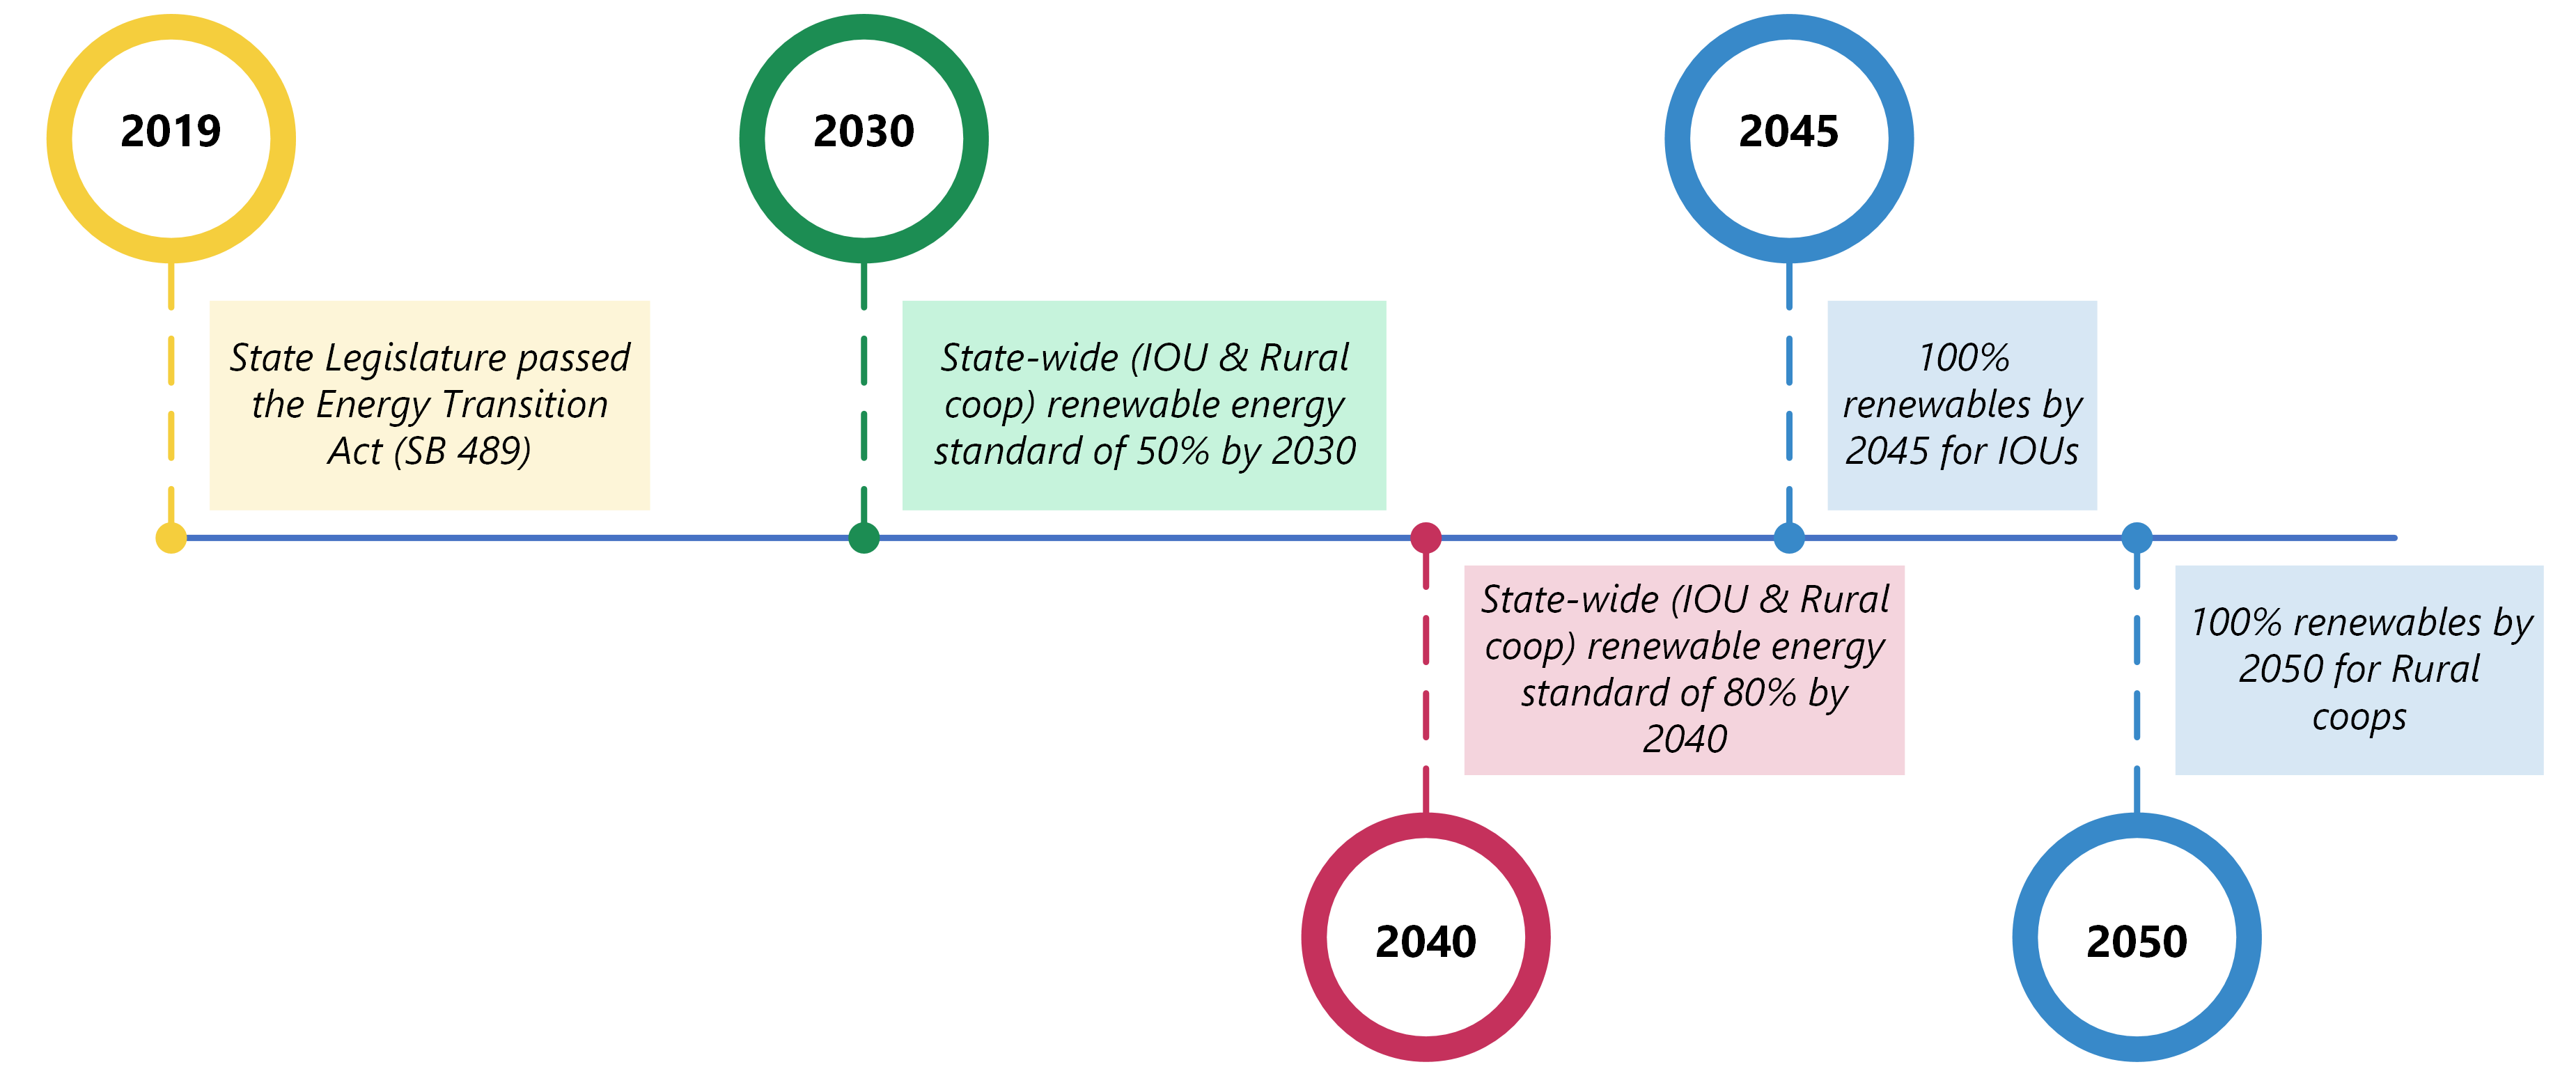
\includegraphics[width=1\textwidth]{figures/nm_eta.png}
    \caption{Timeline of the Energy Transition Act (Senate Bill 489)}
    \label{fig:nm_eta}
\end{figure}

NM is notable for its distinctive demographic composition and climate. Ranking 5th in land area at 121,590 square miles and 36th in population with 2.1 million residents, NM has one of the lowest population densities in the nation \parencite{uscensus2022}.\footnote{NM is the 46th most densely populated state in the nation \parencite{uscensus2022}.} NM is also a majority-minority state, with over 50\% of the population identifies as Hispanic and 11.2\% as Native American \parencite{uscensus2020}.  Around 86\% of the population lives in disadvantaged census tracts defined as overburdened and under-served by the Climate and Economic Justice Screening Tool (CEJST).\footnote{Author's calculation. See \url{https://screeningtool.geoplatform.gov/en/methodology} for a detailed definition of disadvantaged census tracts.} 

In terms of the state's economy, NM Ranks 41st in GDP per capita among the U.S. states.\footnote{Data source: Statista, Real per capita gross domestic product of United States in 2023, by state \url{https://www.statista.com/statistics/248063/per-capita-us-real-gross-domestic-product-gdp-by-state/}.} NM's economy has been significantly reliant on the oil and gas (O\&G) industry since the discovery of the Permian Basin oil fields in the 1920s. The O\&G industry contributes to around 10\% of NM's annual Gross Domestic Product (GDP) and 25\% to 30\% of the state's tax revenue \parencite{eia2023nm, nmlegislative2023}. This dependency on the fossil fuel industry also poses a challenge to the equitable energy transition.

NM is also well-suited to achieve 100\% renewables as NM boasts abundant wind, solar, and geothermal potential. The state's eastern high plains offer significant wind energy opportunities, while NM ranks third in solar energy potential and sixth in geothermal energy potential nationally. In 2022, renewable sources accounted for 42\% of the state's total electricity generation, well on track to achieve the 2030 50\% renewable target \parencite{eia2023energy}.

The interplay between NM's unique demographics, O\&G dependency, and abundant renewable energy resources underlines the importance of exploring equitable energy transition pathways (\autoref{fig:nm_background}). In this research, we focus on solar photovoltaic (PV) and investigate the current state of residential solar PV adoption in NM and its equity implications. 

\begin{figure}[!ht]
    \centering
    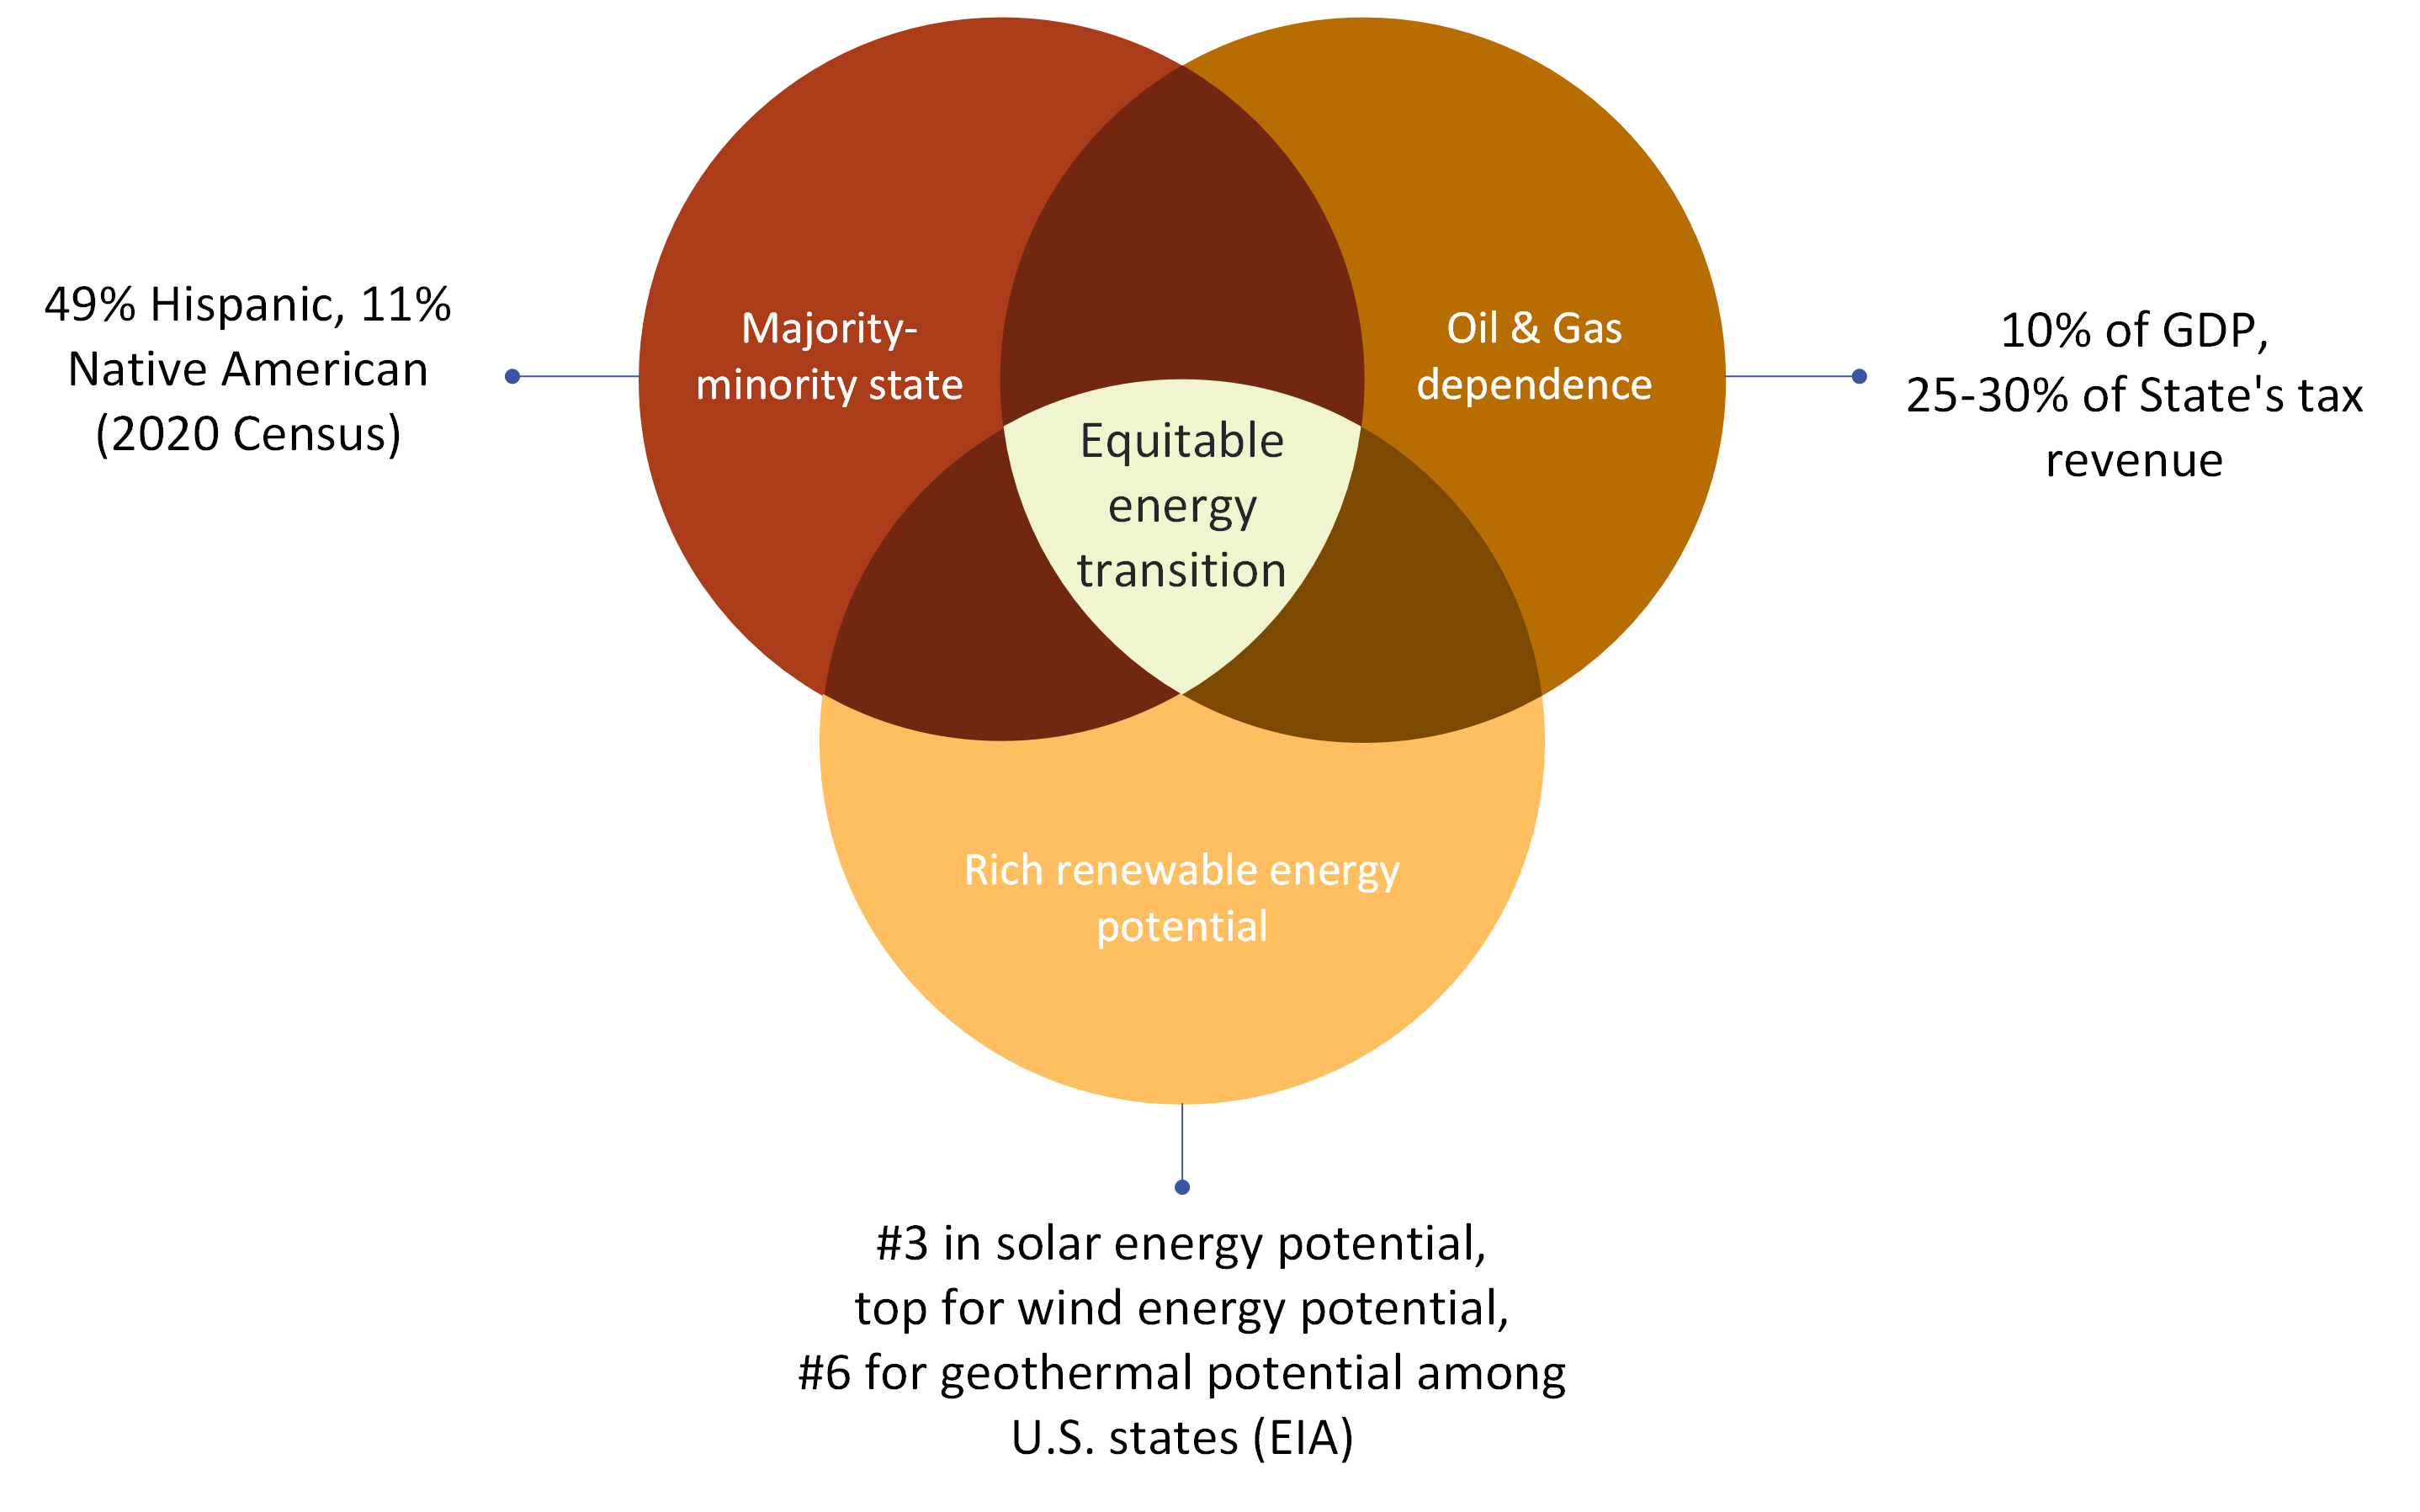
\includegraphics[width=1\textwidth]{figures/nm_background.png}
    \caption{The socioeconomic background of energy transition in New Mexico}
    \label{fig:nm_background}
\end{figure}



\subsection{Equity in energy transition}
\label{section:equity}

In the context of energy transition, the definition of equity encompasses multiple dimensions. The literature can be categorized into three main aspects of equity, namely \textit{access equity}, \textit{adoption equity}, and \textit{distributional equity}. In the following, we review the literature on equitable energy transition with a particular focus on residential solar PV. We also explain the relevance of considering the different aspects of equity in the NM context.

\subsubsection{Access equity}

 Access equity refers to the availability and accessibility of clean energy technologies for all communities, regardless of income, race, or geographic location. \textcite{brockway_inequitable_2021} find using California data that existing grid infrastructure may not be sufficiently robust to handle the increased load from widespread solar PV installations without significant upgrades. This can lead to inequitable access, where certain regions or communities might have lesser ability to connect their solar systems to the grid due to these capacity issues. This finding is relevant in the NM context as solar installations are concentrated in urban areas where in some areas grid infrastructure limits solar installations. For example, in parts of Albuquerque and Rio Rancho, the feeder grids are already at maximum capacity.\footnote{See \url{https://pnm.maps.arcgis.com/apps/webappviewer/index.html?id=cbd3bad85fc64f2180dda652e957bacd} for areas with maximum feeder capacity.} Residents in those communities cannot be approved for new solar installations with grid interconnection until the infrastructure is upgraded.\footnote{In 2021, 2022, and 2023, the Public Service Company of New Mexico (PNM) put 96, 70, and 29 new solar applications on hold, respectively, due to a lack of feeder capacity \parencite{pnm2021,pnm2022,pnm2023}. }

 In addition to grid constraints, other technical barriers, including the lack of suitable roof space or home ownership, or financial barriers, such as high upfront cost, can also limit the ability of some households to adopt solar PV.
 
 \subsubsection{Adoption equity}

Adoption equity in the context of solar PV systems refers to the equitable distribution of solar technology across various socio-economic groups, particularly focusing on income levels, and racial and ethnic groups. Research has consistently highlighted disparities in solar adoption related to these factors. For instance, \textcite{gao_solar_2022} observe a reduction in racial and ethnic disparities in solar PV adoption between 2012 and 2019, yet noted that Asian-, Black-, and Hispanic-majority census tracts still lag behind White-majority tracts in the number of installations. Similarly, \textcite{darghouth_characterizing_2022} identify a significant income-related inequality in U.S. rooftop solar adoption, with more affluent households having a higher likelihood of installing solar systems. They also found that areas with greater racial diversity, higher education levels, and higher owner-occupancy rates showed more equitable solar adoption. Moreover, \textcite{reames_exploring_2021} suggests that although communities of color have marginally lower rooftop solar potential, this does not account for the substantial disparities in adoption rates, highlighting the influence of other non-physical factors.

Researchers also point to supply-side barriers impacting solar equity. \textcite{oshaughnessy_income-targeted_2021} note that solar installers tend to offer fewer quotes to low-income households, thereby reducing their chances of adopting solar technology. This indicates the presence of significant market-driven barriers that could deter solar adoption among economically disadvantaged groups.

 The literature has also examined the effectiveness of various policies to improve equity in solar adoption. \textcite{gao_solar_2022} emphasize that while local and utility-level policies designed to foster solar adoption among diverse populations have benefitted low-income households, their impact remains limited in Black-majority census tracts, suggesting the necessity of addressing non-financial barriers. Meanwhile, \textcite{darghouth_characterizing_2022} argues that decreasing costs of solar PV reduce price-related adoption inequities, but emphasize the need to tackle structural barriers and support diverse installation practices to enhance equity. Financial mechanisms like grants, rebates, and tax credits have been highlighted by \textcite{oshaughnessy_rooftop_2022} as effective tools in encouraging solar adoption among low- and moderate-income households. Additionally, innovative business models such as solar leasing have been shown to significantly boost adoption rates in these communities \parencite{oshaughnessy_impact_2021}.

Examining the issue of adoption equity is particularly relevant in NM given its high share of minority and disadvantaged populations and significant variance in income and education levels. NM also implements generous solar incentives, such as state solar tax credits and utility net energy metering (NEM) policies. Therefore, it is important to evaluate whether these policies alleviate or exacerbate adoption equity in the NM context.

\subsubsection{Distributional equity}

Distributional equity refers to whether the benefits of clean energy incentives are uniformly distributed across different demographic groups. The issue of distributional inequality is not limited to incentives for solar adoption. \textcite{borenstein_distributional_2016} use tax filing data to examine the uptake of four major clean energy tax credits: weatherization (Nonbusiness Energy Property Credit), residential solar (Residential Energy Efficient Property Credit), hybrid and electric vehicles (Alternative Motor Vehicle Credit), and plug-in electric vehicles (Qualified Plug-In Electric Drive Motor Vehicle Credit). They find significant inequities in the distribution of tax credits, with the top income quintile receiving about 60\% of all clean energy tax credits, while the bottom three income quintiles receive about 10\%. \textcite{jacobsen_race_2024} uses survey data from the Residential Energy Consumption Survey (RECS) and finds significant racial and ethnic disparities in the receipt of energy efficiency incentives in the U.S., driven primarily by differences in home-ownership rates. As NM provides state solar tax credits to households, understanding the distributional effect of existing credits provides insights into efficient and equitable policy design.

\subsection[Policy background]{Policy background}

Incentives to promote solar PV adoption in the residential sector have been implemented at different regulatory levels, from federal to service-providing utilities. These incentives play important roles in the households' decision-making of going solar. All incentives are essentially financial, which either lowers the upfront cost of solar investment or reduces the payback period of solar. In the remainder of this section, we review the incentives available to NM households since 2005 for solar PV investments. \autoref{fig:nm_incentive} summarizes the various incentives and their respective policy time spans. For each incentive, we describe the incentive structure, time of initiation and expiration, and eligibility. 

\begin{figure}[H]
    \centering
    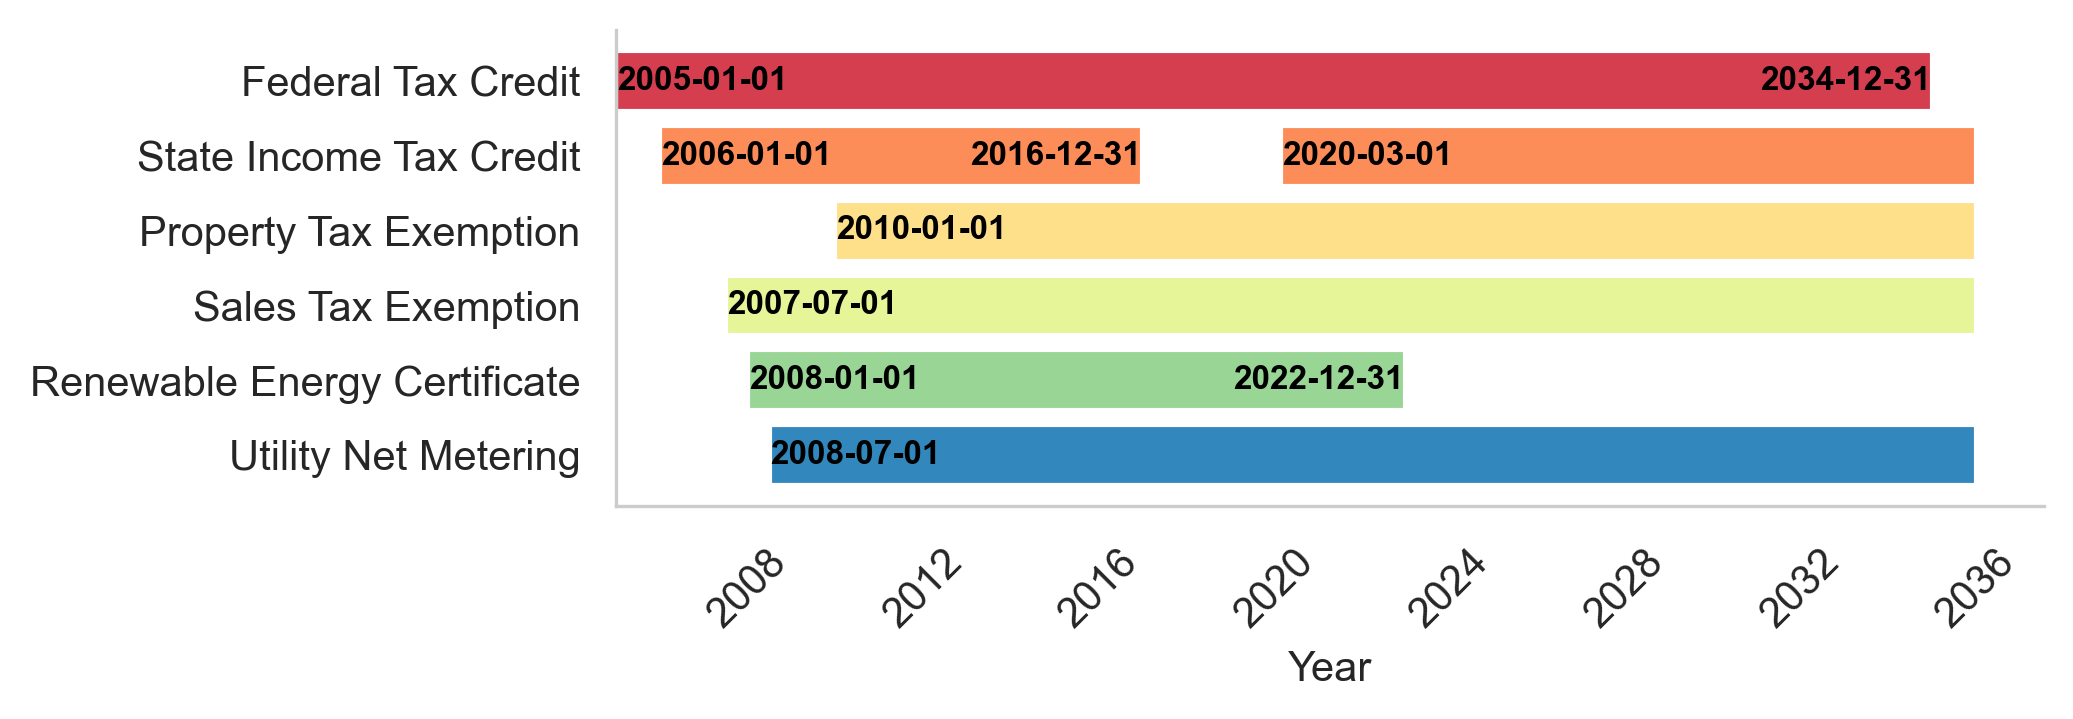
\includegraphics[width=1\textwidth]{figures/policy_timeline.png}
    \caption{Incentives for residential solar PV in New Mexico}
    \label{fig:nm_incentive}
    \begin{flushleft}
        \footnotesize Note: For policies with no definitive end dates, the end date is not displayed in the timeline.
    \end{flushleft}
\end{figure}

\subsubsection{Federal incentives}


The federal tax credit for solar panel installations, also known as the Investment Tax Credit (ITC), was initially introduced in the Energy Policy Act in 2005. It provided a tax credit of 30\% for residential and commercial solar energy installations. ITC was extended multiple times and maintained a 30\% credit for solar installations through 2019. The tax credit percentage was stepped down in 2020, where the systems installed in 2020 and 2021 were eligible for a 26\% tax credit \parencite{doeitc}. ITC was originally set to phase down after 2022 (26\% in 2022, 22\% in 2023, 0\% by 2024) before the introduction of the Inflation Reduction Act (IRA) in 2022. IRA extended the ITC, now known as the Residential Clean Energy Credit, which provides a 30\% tax credit from 2022 through 2032. The credit rate phases down to 26\% in 2033 and 22\% in 2034, unless otherwise noted. The federal tax credit places no limit on the total amount claimed, and any credit exceeding tax liability can be carried forward to future tax years \parencite{irs}.

\subsubsection{State incentives}

\textbf{Solar tax credit}

Since the early 2000s, the role of renewable energy in mitigating greenhouse gas emissions and addressing climate change has become increasingly evident. In response to this growing awareness, NM introduced the Solar Market Development Tax Credit (SMDTC) in 2006. This initiative was aimed at encouraging the adoption of solar energy through financial incentives. From January 1, 2006, until December 31, 2016, the SMDTC provided a 10\% tax credit on the total installation costs of solar panel systems, with a cap of \$9,000 per taxpayer per taxable year. 

Recognizing the continued importance of fostering renewable energy adoption, NM reinstated this incentive in 2020 with the introduction of the New Solar Market Development Tax Credit (NSMDTC). Effective from March 1, 2020, this revised program also offers a 10\% tax credit on the total installation costs, but with a reduced maximum credit amount of \$6,000. To manage fiscal impacts, the total tax credit issuance was initially capped at \$8 million for the tax years 2020 and 2021, and increased to \$12 million annually from 2022. Due to high demand, this cap has been reached consistently each year, leading to a further increase to \$30 million in 2024.\footnote{In 2021, 2022, and 2023, the credit cap was reached. \url{https://nm-emnrd.maps.arcgis.com/apps/dashboards/e882d2ccd57e4a99bc6d2a4314fcd3bb}}

The program features no income threshold for eligibility, and initially, any unused credit exceeding the taxpayer’s liability could be carried over for up to five consecutive years. However, in a significant policy evolution, the tax credit became refundable in 2024, enhancing its accessibility by allowing taxpayers to receive a refund for any credit amount that surpasses their tax liability \parencite{nmsmdtc}.

\noindent\textbf{Property tax exemption}

Under House Bill 233, enacted by the NM legislature in 2010, residential solar systems are not treated as physical improvements and therefore do not increase the value of the property for property tax purposes. However, future assessments can include the value of a solar energy system if the property is sold \parencite{propertytax}. This exemption provides a financial incentive for homeowners since installing solar PV increases property value on the housing market without incurring additional property taxes.


\noindent\textbf{Sales tax exemption}

The NM Gross Receipts Tax Exemption policy for solar energy systems, effective since 2007, allows businesses to deduct receipts from selling solar equipment or installation services \parencite{NMStat2021}. Essentially, for consumers, there is no sales tax on top of the cost of solar installation, which reduces the financial burden on solar adopters.


\noindent\textbf{Renewable energy certificates}

The NM Renewable Energy Certificate (REC) policy for solar PV is part of the state's broader Renewable Portfolio Standard (RPS). The RPS requires that IOUs must secure 50\% of their capacity through carbon-free renewables by 2030 and 100\% by 2045. For rural electric cooperatives, the goals are 40\% by 2025, 50\% by 2030, and 100\% by 2050. The IOUs in NM thus offered Renewable Energy Certificate (REC) purchase agreements to solar owners for a limited time to count residential solar generation toward their required RPS. The Public Service Company of New Mexico (PNM) offered a Solar Renewable Energy Certificate (SREC) program that awards systems a stepped purchased rate for the energy generated for residential systems. This program was discontinued at the end of 2022 \parencite{pnmrec}. The El Paso Electric Company (EPE) offered a tiered REC purchase rate for systems installed before 2017, which ended on December 31, 2020 \parencite{eperec, eperecmid}.\footnote{Details on the purchase agreements can be found on the respective company's websites.}

\subsubsection{Utility incentives}

Utility companies in NM, including IOUs, rural cooperatives, and public utilities, are mandated by the NM Public Regulatory Commission (NMPRC) to offer net energy metering (NEM) programs to solar customers. Under NEM, solar customers who generate excess electricity with their solar panel systems can send it back to the grid and receive credits. These credits can be used to offset future electricity use.\footnote{For example, if the solar panels generate more electricity during the day than the household consumes, the excess electricity is sent back to the grid, and the meter runs backward, creating a credit. At night, when solar panels do not produce electricity, the household consumes electricity from the grid and the meter runs forward.} However, the details of the NEM program vary by utility. For example, PNM offers a net metering program for all residential solar systems. For small PV systems (inverter capacity lower than 10 kW-AC), any excess generation for the month (when monthly usage is lower than total monthly generation) is credited to the customer’s account and can be used for future billing cycles, never expiring unless the account is closed. Excess generation from large PV systems (inverter capacity greater than 10 kW-AC) is paid each month at the predetermined energy purchase rate for that month \parencite{pnmnet}. EPE offers net metering for all systems within a billing cycle, but all excess generation for the month is paid out to customers at the predetermined purchase rate \parencite{epenet, epenetmid}. The purchase rate for the credits is typically lower than the retail electricity price for all utilities.\footnote{For example, in 2023, the PNM power purchase rate ranged from 3 to 12 cents per kilowatt hour (kWh), depending on the month, while the retail rate was 7.8 cents per kWh for the first 450 kWh per month, increasing to 15 cents per kWh thereafter.} The differences in NEM incentives provide a quasi-experimental setting to study how NEM policy design incentivizes residential solar adoption. 

%%%%%%%%%%%%%%%%%%%%%%%%%%%%%%%%%%%%
% \section{Current trend  and distribution of residential solar in New Mexico}
\customsection{Current trend  and distribution}{Current trend  and distribution of residential solar in New Mexico} %header shows the name in first braces

In this section, we utilize detailed solar installation data collected from state agencies and utilities to illustrate the trends and distribution of solar installations in NM. Our focus is on the distribution across geographical areas, income groups, and racial and ethnic groups for both installation counts and system capacities.

\subsection{Data description}
\label{section:data_collect}

To provide a comprehensive overview of solar installations in NM, we assembled a unique dataset from various public and restricted sources. This dataset includes system-level characteristics, housing characteristics, census tract-level demographics, and spatial data on climate and community types. The following sections detail the dataset components.

\subsubsection{Installation data}

We obtain system-level solar installation data from three sources: the New Mexico Energy, Minerals, Natural Resources Department (EMNRD), the NMPRC document archive eDocket database, and individual utilities. 

EMNRD oversees the state solar tax credit claims under the SMDTC and NSMDTC programs. Their data includes all systems that were approved for the state tax credits between the programs' active periods (2006-2016 and 2020 onwards). This data, acquired through a non-disclosure agreement, provides details on the installation location, grid connection date, system size, installer name, system cost, and approved state credit amount, encompassing 20,159 unique residential systems.

The NMPRC eDocket database contains records of annual compliance filings by state-regulated utilities (IOUs and rural cooperatives) under Rule 17.9.570.13(G) NMAC.\footnote{Details of Rule 17.9.570 can be found here: \url{https://www.srca.nm.gov/parts/title17/17.009.0570.html}.} This rule mandates utilities to report the name and location of interconnected solar systems, annual purchases from these systems, and any rejected interconnection applications. Due to varying data quality, we obtain data of the two largest IOUs in the state, PNM and EPE, and one rural cooperative, Socorro Electric Coop (SEC). Together, they account for over 90\% of solar customers in NM, providing data on system location, interconnection date, and installed capacity for 50,416 residential systems.

Public utilities, not subject to NMPRC rulings, provided solar system data directly. We obtain data from the Los Alamos Department of Public Utilities (LADPU) for the 427 residential solar systems in their service area.


\subsubsection{Housing characteristics data}

We scrap housing characteristics data from Zillow using the addresses in the installation data. This data includes variables such as year built, number of bedrooms and bathrooms, estimated home value (Zestimate), living area size, lot size, parking features, heating and cooling technologies, and geographic coordinates.\footnote{NM is a non-disclosure state, meaning the actual transaction price of homes is not public information.} Housing information was available for 65,125 systems in the combined installation dataset.

\subsubsection{Census tract-level demographics data}

Using the geographical information from the housing data (longitude and latitude), each system was placed in a census tract using the Census Bureau’s tract shape file. We gathered census tract-level demographic variables from the 2010 and 2020 Decennial Census and the American Community Survey from 2010 to 2022. The demographic data includes the following variable categories: 1) housing characteristics (total housing units, occupancy rate, owner occupancy rate, average number of rooms and housing size, main energy source, mortgage rate, housing value, and age of housing); 2) racial composition (racial diversity, percentages of white, Native American, and Hispanic populations); and 3) other demographics (percentage of male population, age distribution, education level, total population, area median income, and urban/rural classification).

\subsubsection{Other relevant data}

We complemented the main dataset with utility-level average annual electricity prices from the Energy Information Administration (EIA) \parencite{eiaprice}, spatial weather data from Solargis, including Global Horizontal Irradiation (GHI) and average annual temperature \parencite{solargis}, and the community disadvantage status from the CEJST \parencite{cejst}.

In summary, our comprehensive dataset contains 54,462 unique solar installations (full sample) in NM, 49,993 of which have detailed geographical information (restricted sample). We use the full sample in the subsequent analysis when geographical information is not required and use the restricted sample when spatial analysis is needed.

\subsection{Installation time trend}
 
NM has experienced exponential growth in residential solar installations since 2000. As shown in \autoref{fig:culmulative_capacity}, the total installation capacity in 2023 (280 MW) almost doubled that in 2020 (141 MW). By 2023, residential solar accounted for 14.8\% of the state’s total solar capacity \parencite{seia2023nm}.

\begin{figure}[!ht]
    \centering
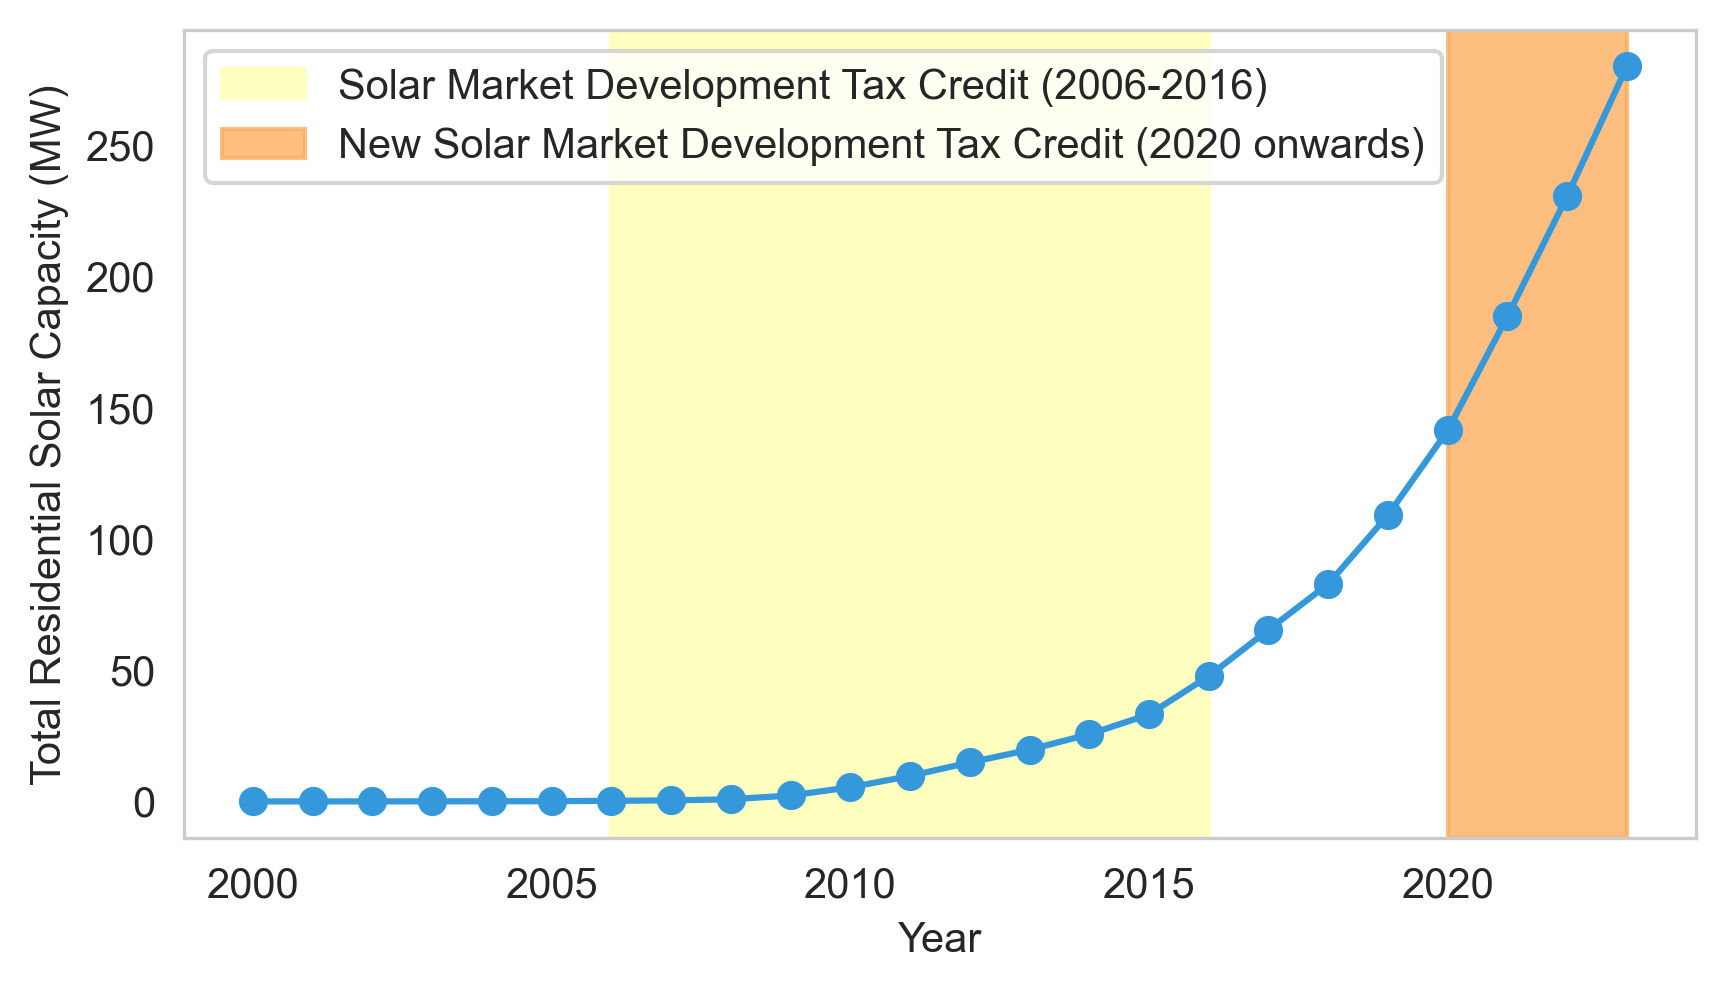
\includegraphics[width=0.9\textwidth]{figures/cumulative_capacity.png}
    \caption{Cumulative residential solar capacity from 2000 to 2023}
    \label{fig:culmulative_capacity}
    \begin{flushleft}
        \footnotesize Note: The line chart shows the cumulative residential solar capacity since 2000 in megawatts (MW). The shaded areas illustrate the policy period of the first and second state solar tax credits.  
    \end{flushleft}
    
\end{figure}


The rapid growth in residential solar can partially be attributed to the significant reduction in the cost of solar panels. \autoref{fig:installation_count} shows the annual installation count in relation to the unit price of the installation. The installation price per kilowatt (kW) of solar PV capacity in 2023 is less than one-third of the price in 2007, making solar an affordable energy source for many households.

State solar tax credits, combined with federal and other incentives, have also facilitated the growing adoption of solar. Figures \ref{fig:culmulative_capacity} and \ref{fig:installation_count} show that in years with tax credits, the adoption level is high, especially when unit prices are lower.

\begin{figure}[H]
    \centering
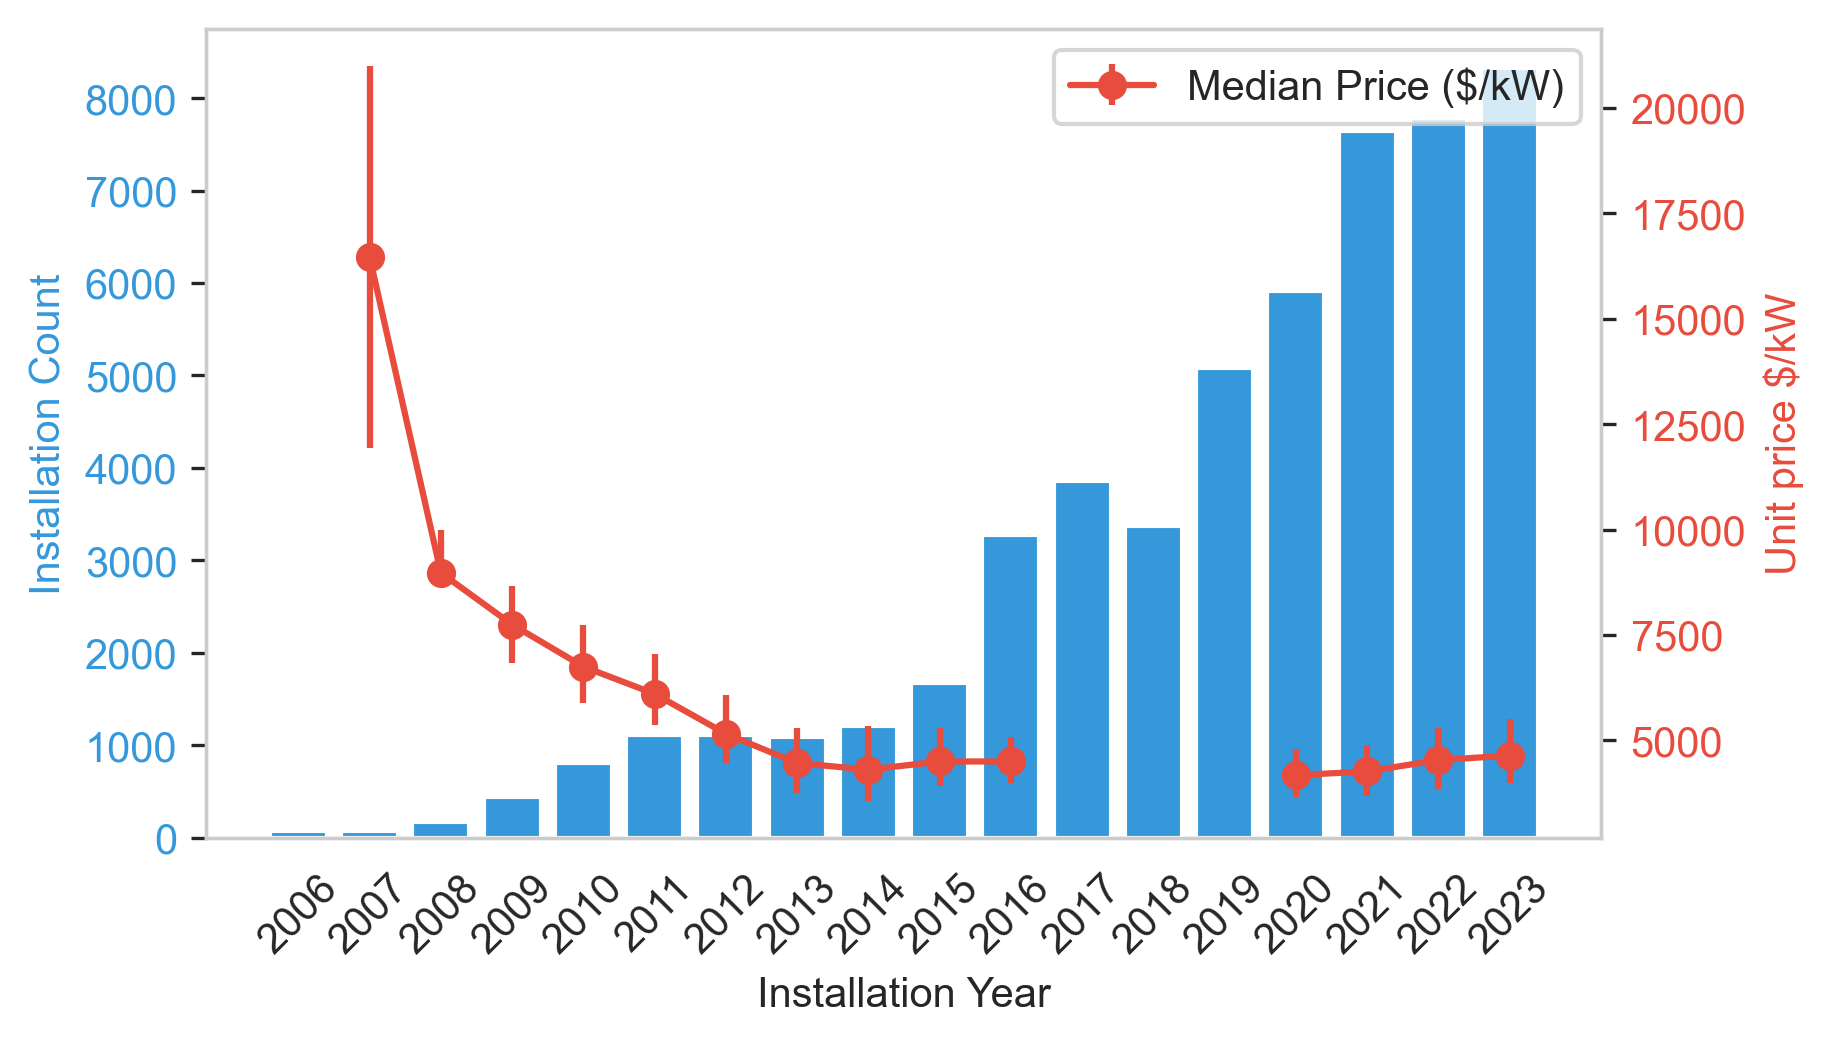
\includegraphics[width=1\textwidth]{figures/installation_count_price.png}
    \caption{Annual solar installation count and unit price in New Mexico}
    \label{fig:installation_count}
    \begin{flushleft}
        \footnotesize The error bars show the 25\% to 75\% range of the unit prices (\$/kW). The installed price ranges exclude any systems with battery storage. In the years 2017 to 2019, the state’s solar tax credit program was not available. Therefore, price information is missing for those years.
    \end{flushleft}
\end{figure}

\subsection{Distribution of solar installation}

\subsubsection{Spatial distribution}
\label{subsec:Spatial distribution}

The growth in solar adoption is not uniformly distributed across NM. \autoref{fig:tract_map} shows the total installations by census tract. It is evident that current solar installations are concentrated in the most populous cities of NM, namely Albuquerque, Santa Fe, and Las Cruces. Even after adjusting for population density (\autoref{fig:install_kpop}), there is still a higher installation per thousand people in these cities, indicating an urban/rural disparity in solar adoption.

\begin{figure}[!ht]
    \centering
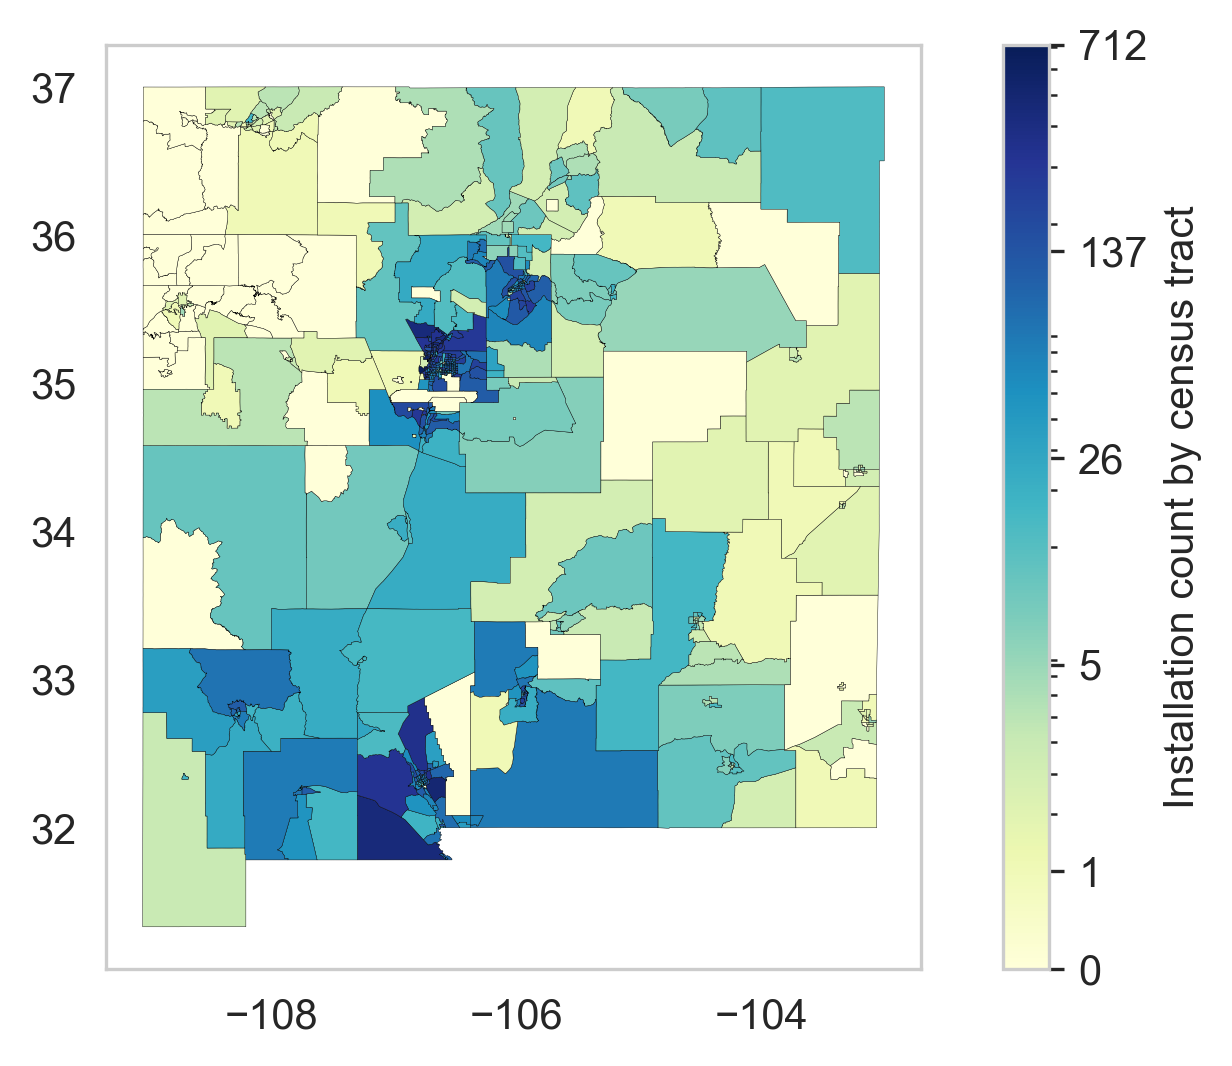
\includegraphics[width=0.7\textwidth]{figures/tract_count_map.png}
    \caption{Total installation count by census tract}
    \label{fig:tract_map}
    \begin{flushleft}
        \footnotesize Note: The total installation count is up to the end of 2023 for each census tract. The census tracts are defined in the 2020 Decennial Census. The legend is on logarithmic scale.
    \end{flushleft}
\end{figure}

\autoref{fig:disadvantage_installation} illustrates the distribution of installations with respect to disadvantaged census tracts within NM. Disadvantaged census tracts are defined as “census tracts that are overburdened and underserved” by the Justice40 Initiative \parencite{justice40}. While 86\% of the population in NM lives in disadvantaged communities, less than 29\% of the solar installations are within those communities (orange dots in the figure).

\begin{figure}[H]
    \centering
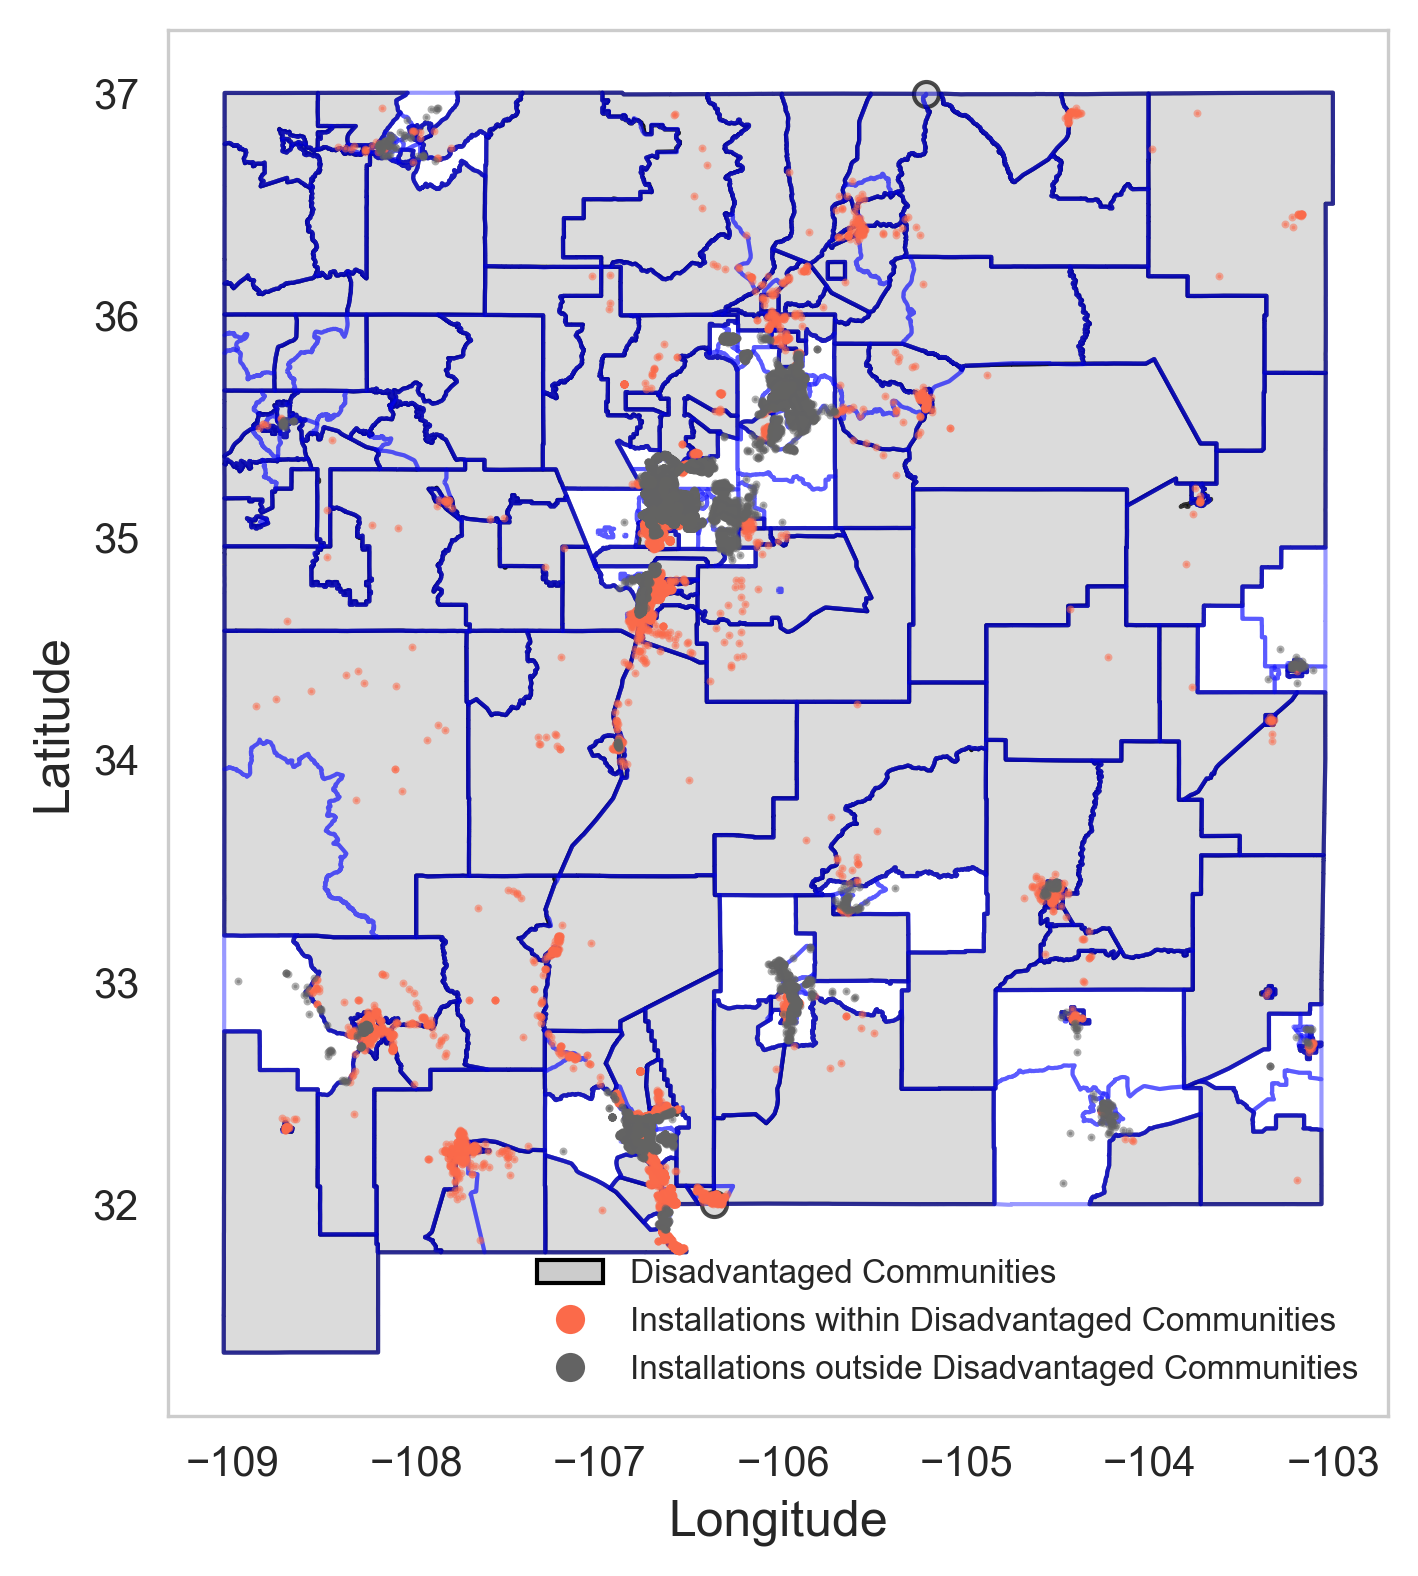
\includegraphics[width=0.7\textwidth]{figures/disadvantage_installation.png}
    \caption{Installation within and outside disadvantaged communities}
    \label{fig:disadvantage_installation}
        \begin{flushleft}
        \footnotesize Note: Disadvantage communities shape file retrieved from the Climate and Economic Justice Screening Tool \url{https://screeningtool.geoplatform.gov/en/#10.84/36.2534/-104.868}. Census tracts that are overburdened and underserved are highlighted as being disadvantaged on the map.
    \end{flushleft}
\end{figure}


\subsubsection{Income distribution}

Consistent with existing research, census tracts in NM with higher area median income (AMI) also have more households installing solar, even when adjusted for population (see \autoref{fig:comparative_histogram_installation}). \autoref{fig:population_ami_count} reveals a positive correlation between AMI and installation per thousand population.


\begin{figure}[h]
    \centering
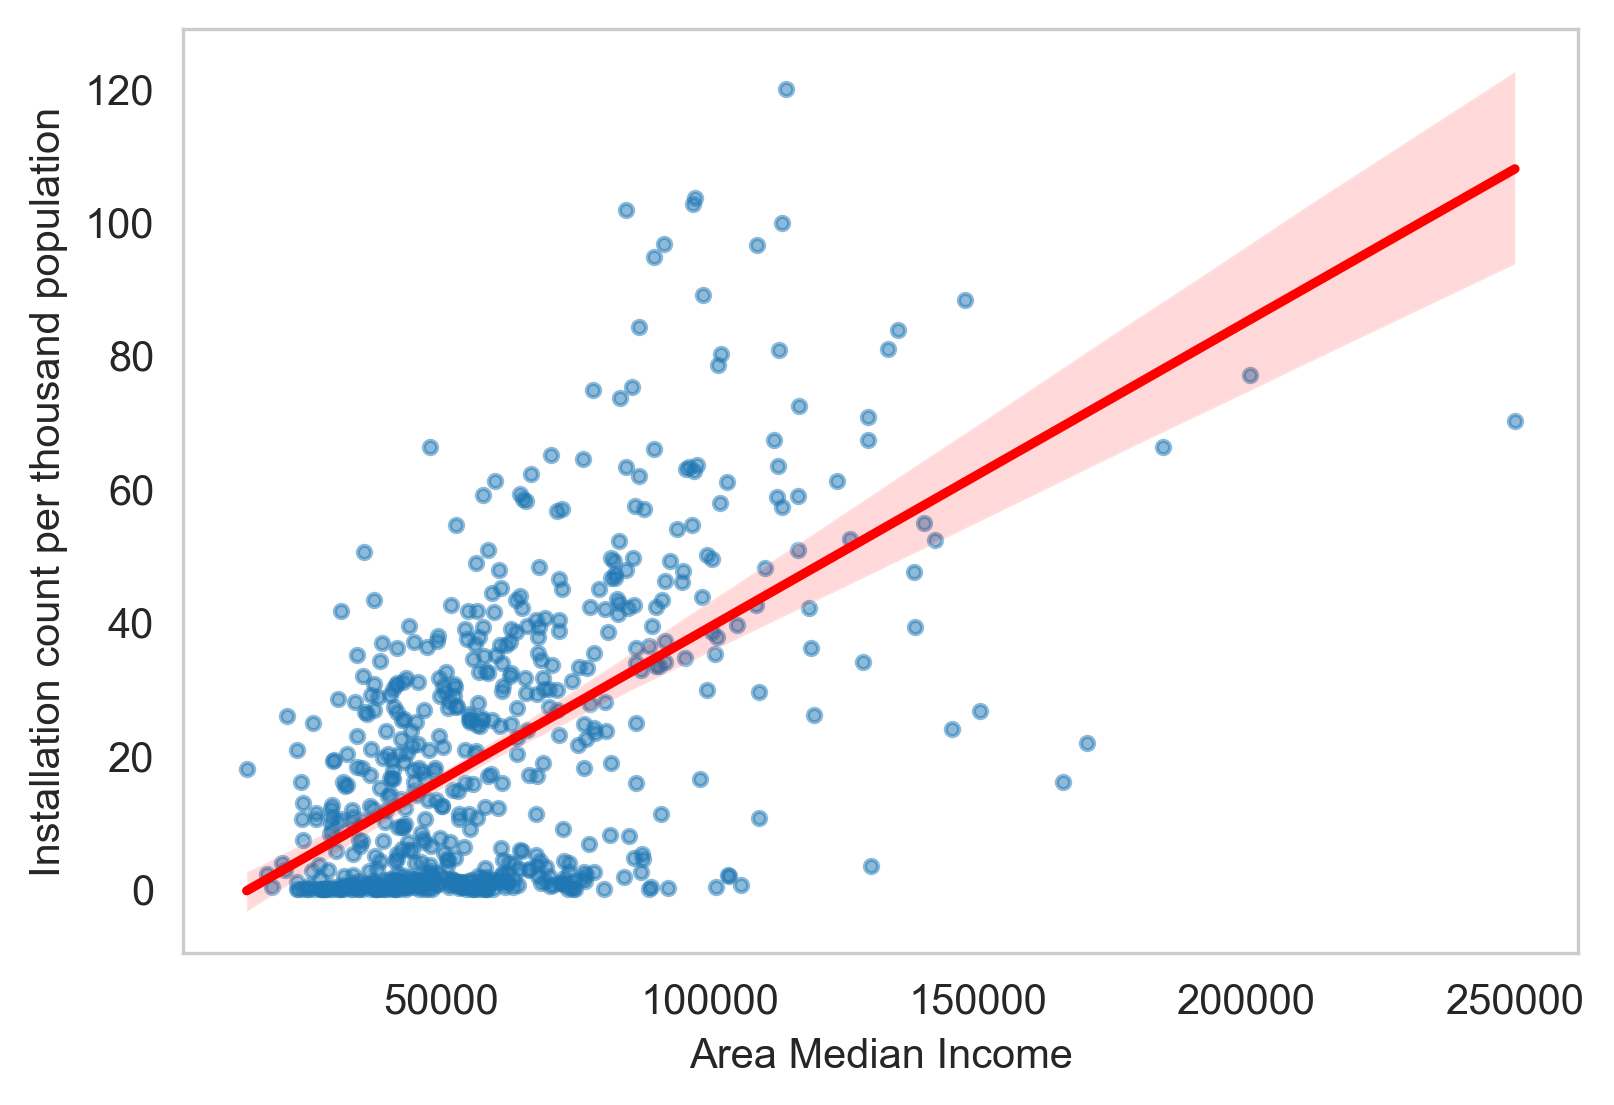
\includegraphics[width=0.9\textwidth]{figures/population_ami_count.png}
    \caption{Installation per thousand population by area median income}
    \label{fig:population_ami_count}
        \begin{flushleft}
        \footnotesize Note: The population and area median income (AMI) are based on 2022 data from the American Community Survey 1-year data. Census tracts with an AMI higher than 250,000 are capped at 250,000. The shaded area around the regression line represents the 95\% confidence interval.
    \end{flushleft}
\end{figure}

Analyzing the total solar installations from 2010 to 2022 by income quartile (\autoref{fig:comparative_histogram_installation}), we observe distinct patterns in the distribution across different income levels. The histogram for the bottom income quartile reveals a highly left-skewed distribution, indicating a concentration of census tracts with fewer installations. Conversely, the top income quartile demonstrates a more evenly spread distribution across various levels of installation counts, suggesting a broader uptake of solar technology among higher-income tracts.

\begin{figure}[!ht]
    \centering
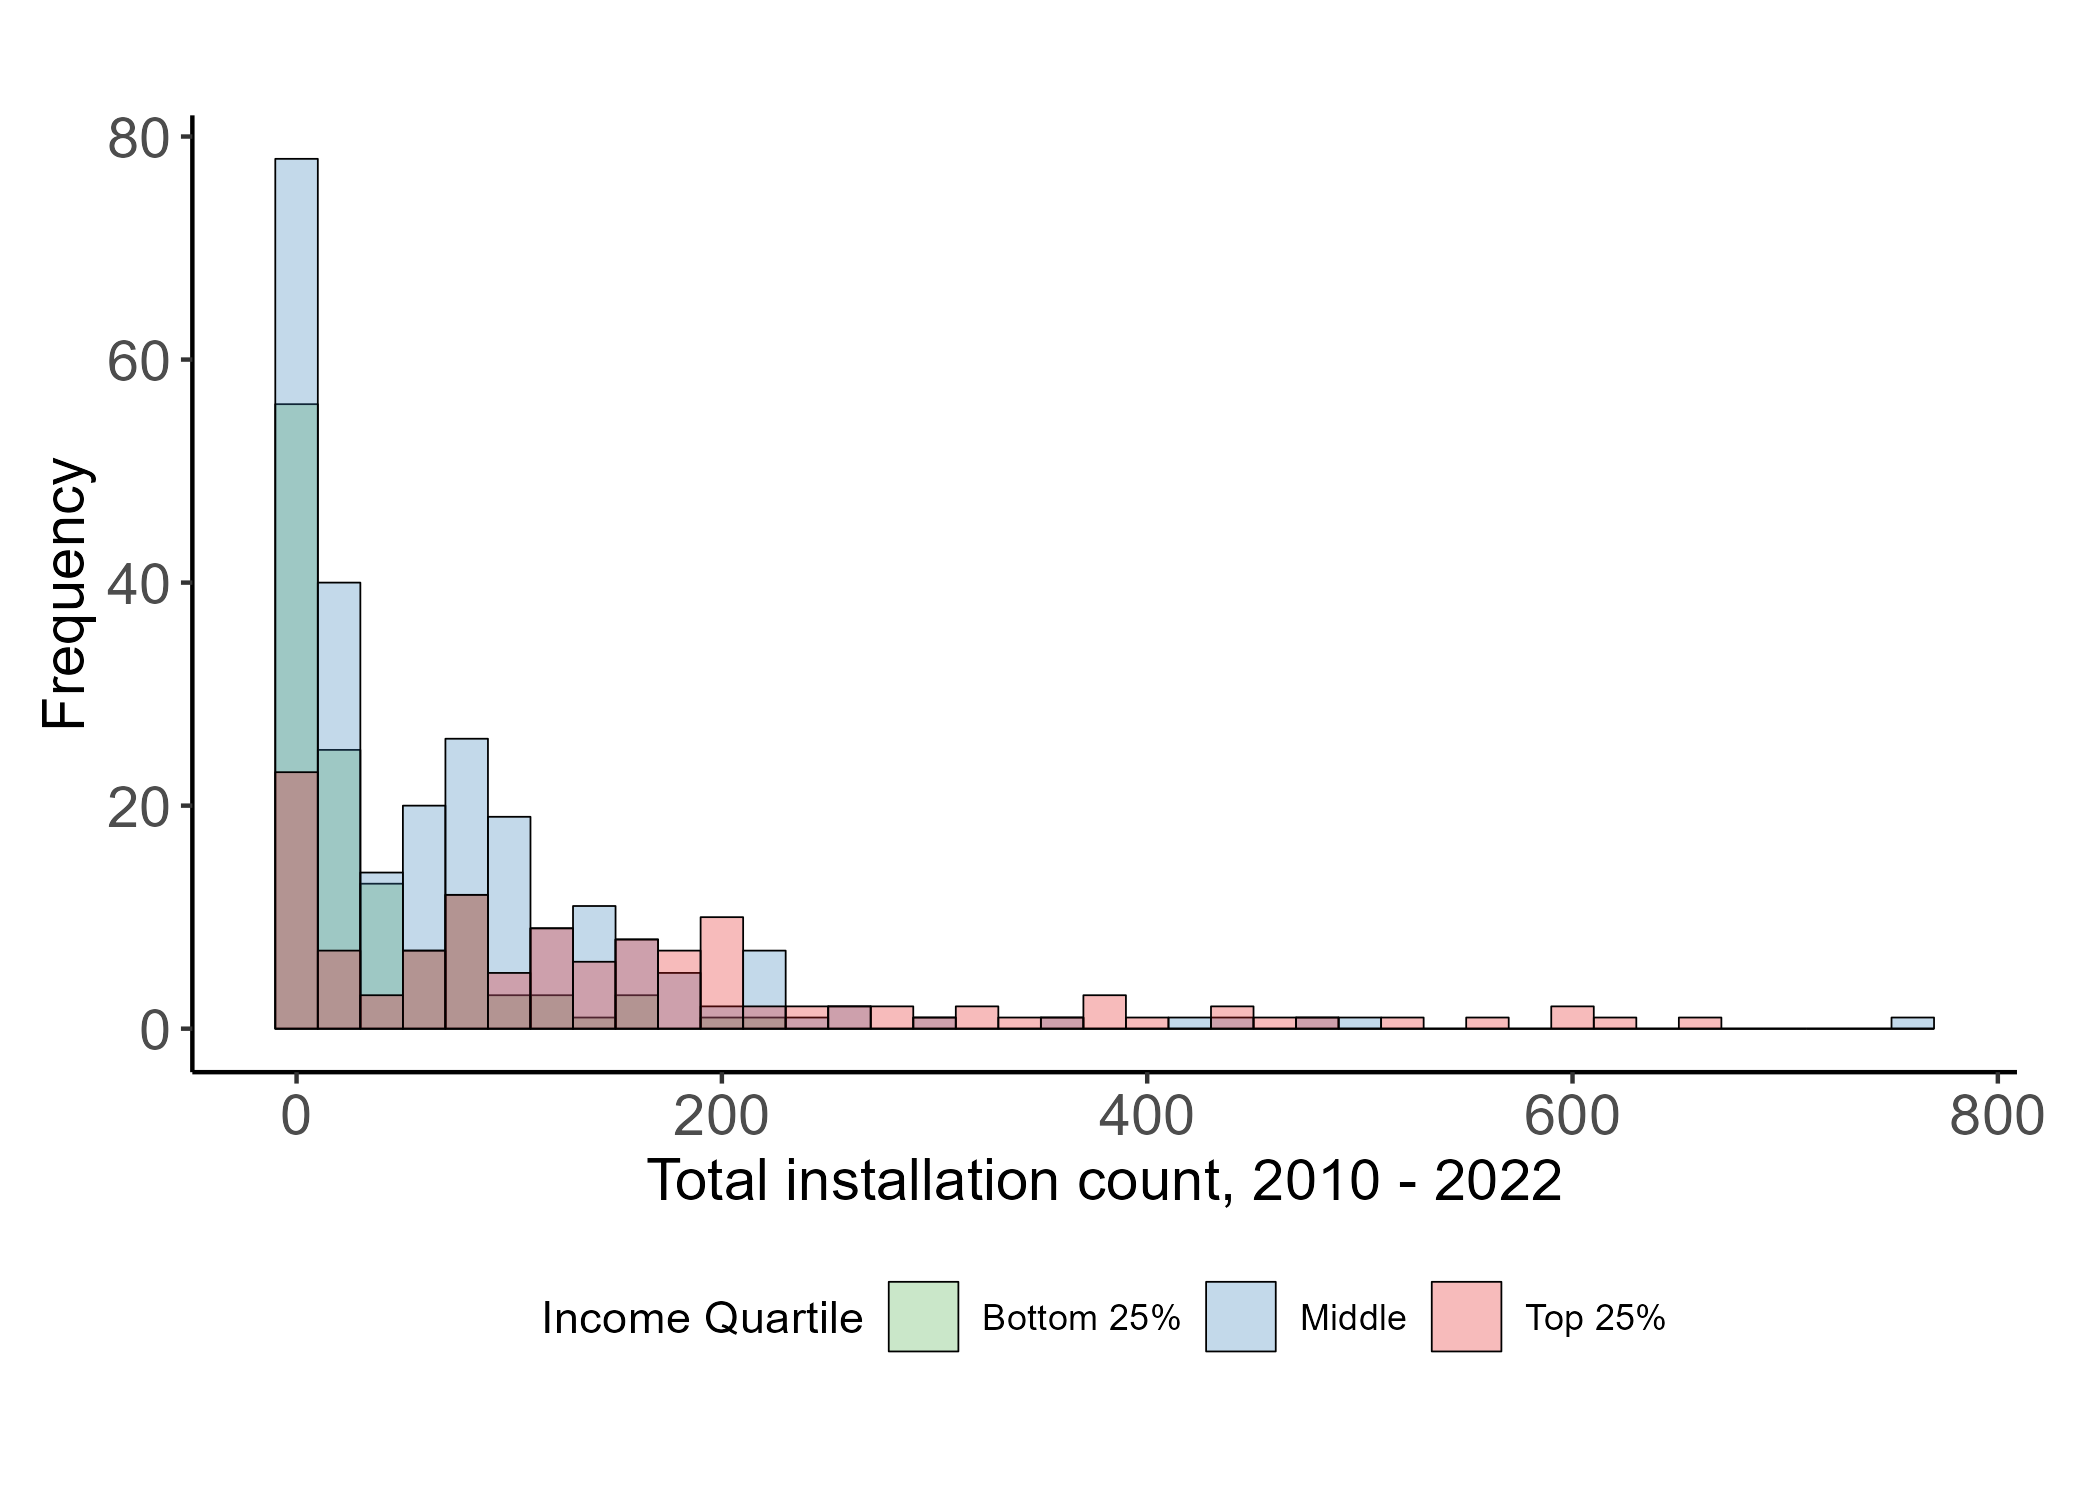
\includegraphics[width=0.9\textwidth]{figures/comparative_histogram_installation.png}
    \caption{Census tract total installation by income quartile}
    \label{fig:comparative_histogram_installation}
        \begin{flushleft}
        \footnotesize Note: The income quartile classification is based on the average census tract area median income from 2010 - 2022. The total installation is the sum of installation in each census tract from 2010 - 2022.  
    \end{flushleft}
\end{figure}

\subsubsection{Racial and ethnic distribution}

New Mexico features a racially and ethnically diverse composition. According to the 2020 Census, 51\% of the population identifies as White alone \parencite{uscensus2020}. Other significant groups include American Indian and Alaska Native (10\%), Black or African American (2.2\%), Asian (1.8\%), individuals identifying as Some Other Race alone (15.0\%), and those identifying as two or more races (19.9\%). The state’s population is nearly evenly divided between Hispanic (47.7\%) and non-Hispanic (52.3\%), with White non-Hispanics making up 36.5\%.

Of the 612 census tracts in NM, 64\% are White-majority (where more than 50\% of the population identifies as White alone), and 38\% are Hispanic-majority. An analysis of the total installation count by majority status (\autoref{fig:installation_race}) shows a notable concentration of installations in White-majority census tracts over the years. The disparity between Hispanic-majority and non-Hispanic-majority tracts is less pronounced, with non-Hispanic tracts having slightly higher installation counts. This trend is further elaborated in \autoref{fig:population_quintiles}, which divides the data into five bins based on population shares, rather than majority status.

\begin{figure}[!ht]
    \centering
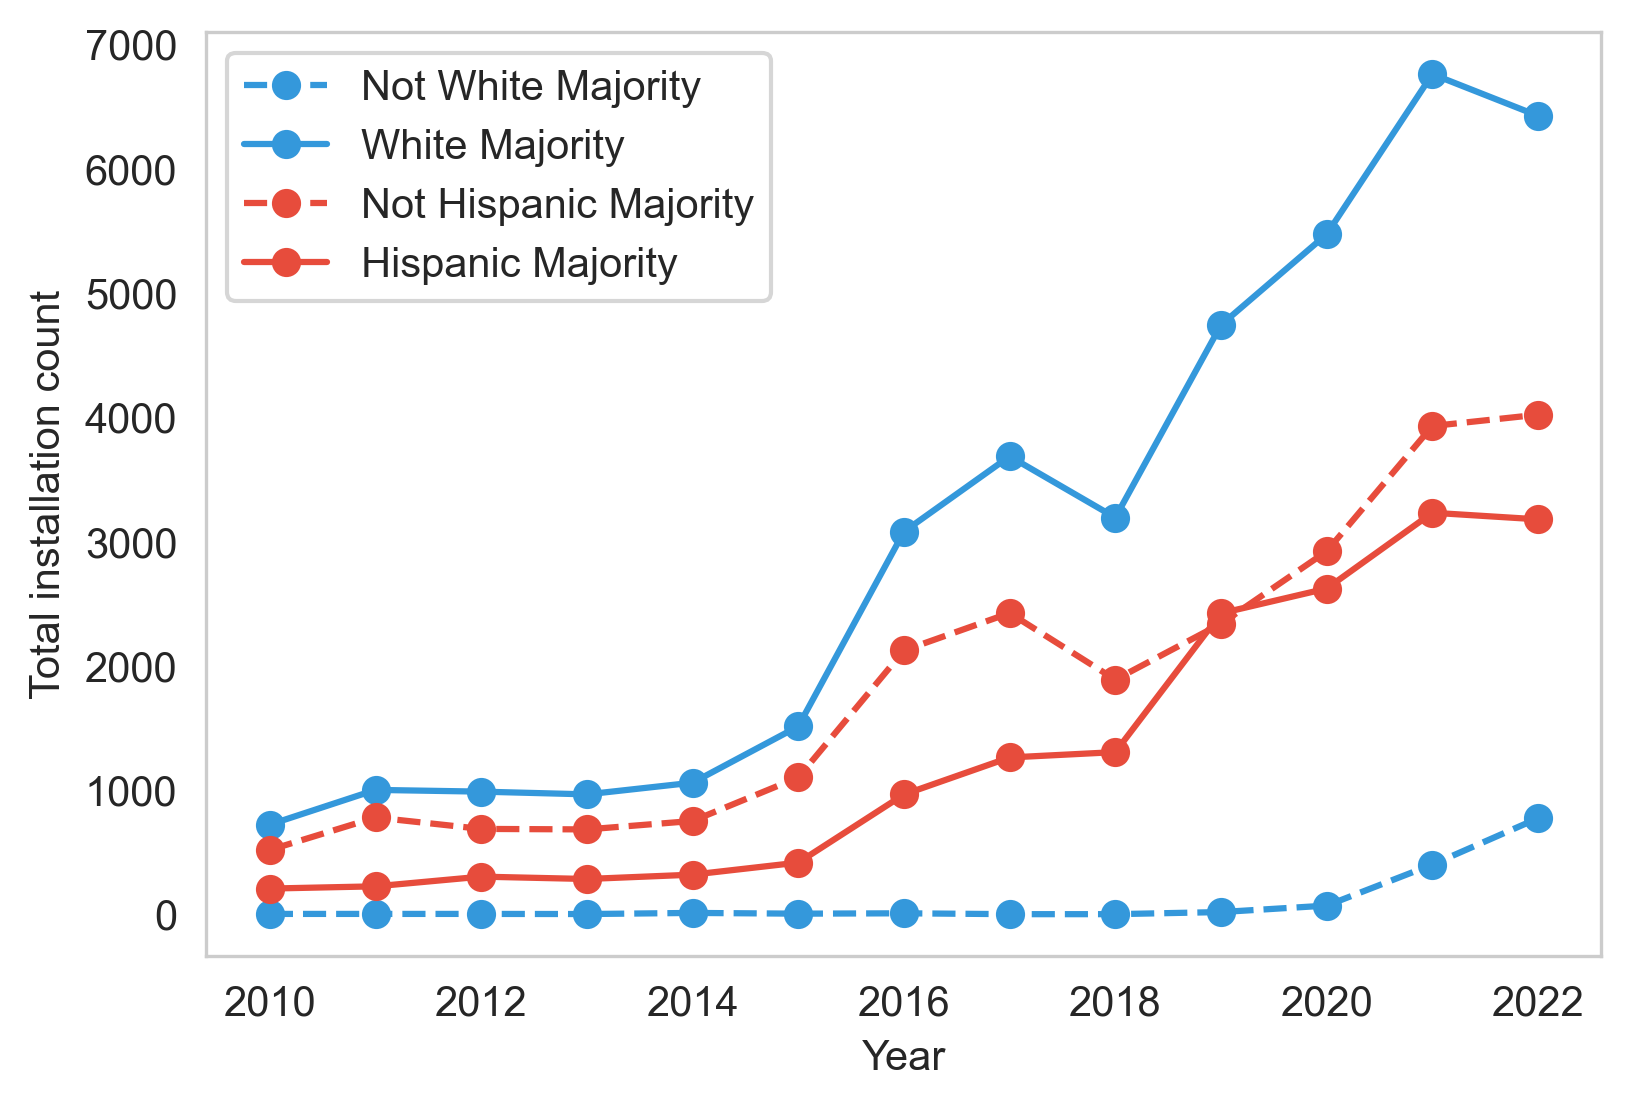
\includegraphics[width=0.9\textwidth]{figures/installation_by_race.png}
    \caption{Annual installation by racial majority group}
    \label{fig:installation_race}
        \begin{flushleft}
        \footnotesize Note: White majority refers to census tracts where more than 50\% of the population identifies as White alone. Hispanic majority refers to census tracts where more than 50\% of the population identifies as Hispanic.
    \end{flushleft}
\end{figure}



\subsubsection{Capacity distribution}

The capacity of installed systems varies among solar households. \autoref{fig:capacity_density} displays the distribution and cumulative distribution function (CDF) of system capacities (in kW). Most system capacities are clustered between 2 kW and 8 kW, with half of the systems below 5 kW and 95\% below 10 kW.


\begin{figure}[!ht]
    \centering
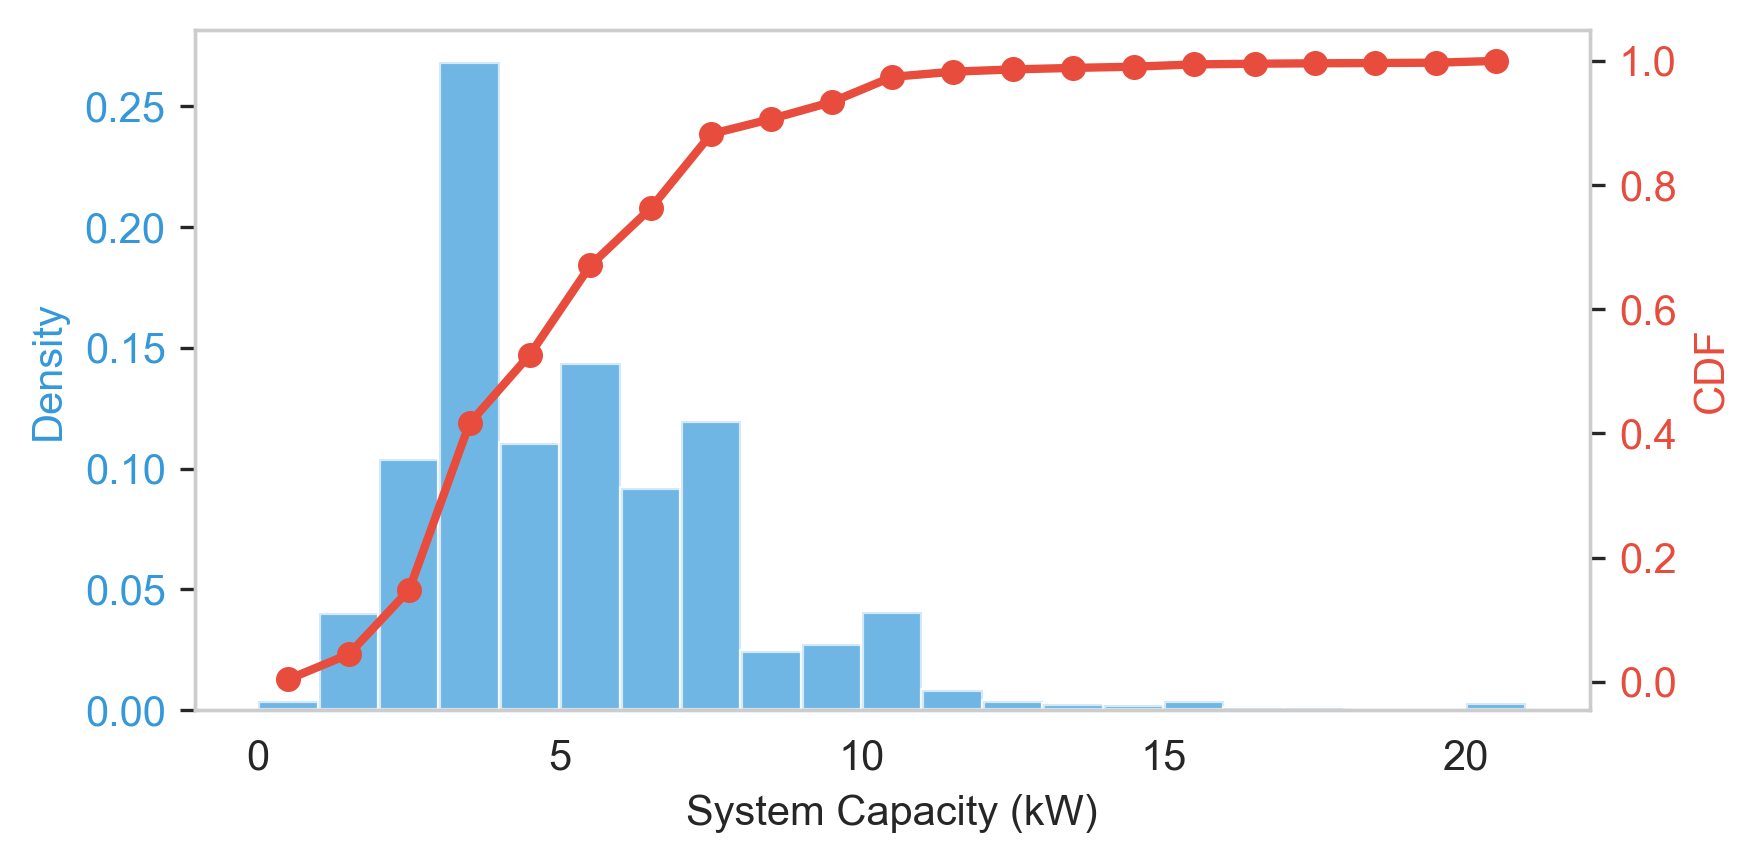
\includegraphics[width=1\textwidth]{figures/capacity_density_cdf.png}
    \caption{Distribution  of installed solar PV system capacity}
    \label{fig:capacity_density}
        \begin{flushleft}
        \footnotesize Note: Systems with capacity greater or equal to 20kW are grouped together. 
    \end{flushleft}
\end{figure}

The choice of system capacity can be influenced by many factors, including household size and utility incentives. \autoref{fig:capacity_size} depicts the relationship between installed system capacity (in kW) and the size of the living area of the home (in square feet), differentiated by utilities. It shows that as the housing size increases, the installed system capacity tends to increase. However, the intensity of this correlation varies by utility. Systems within the PNM service area have the highest slope compared to those served by EPE or other utilities. This difference could be attributed to variations in utility-level incentives (e.g., NEM policies) or correlations between utility service areas and other factors such as urban/rural or installer characteristics. It is notable that the shares of systems installed within the PNM, EPE, and other service areas are 77.9\%, 16.7\%, and 5.4\%, respectively.
 
\begin{figure}[!ht]
    \centering
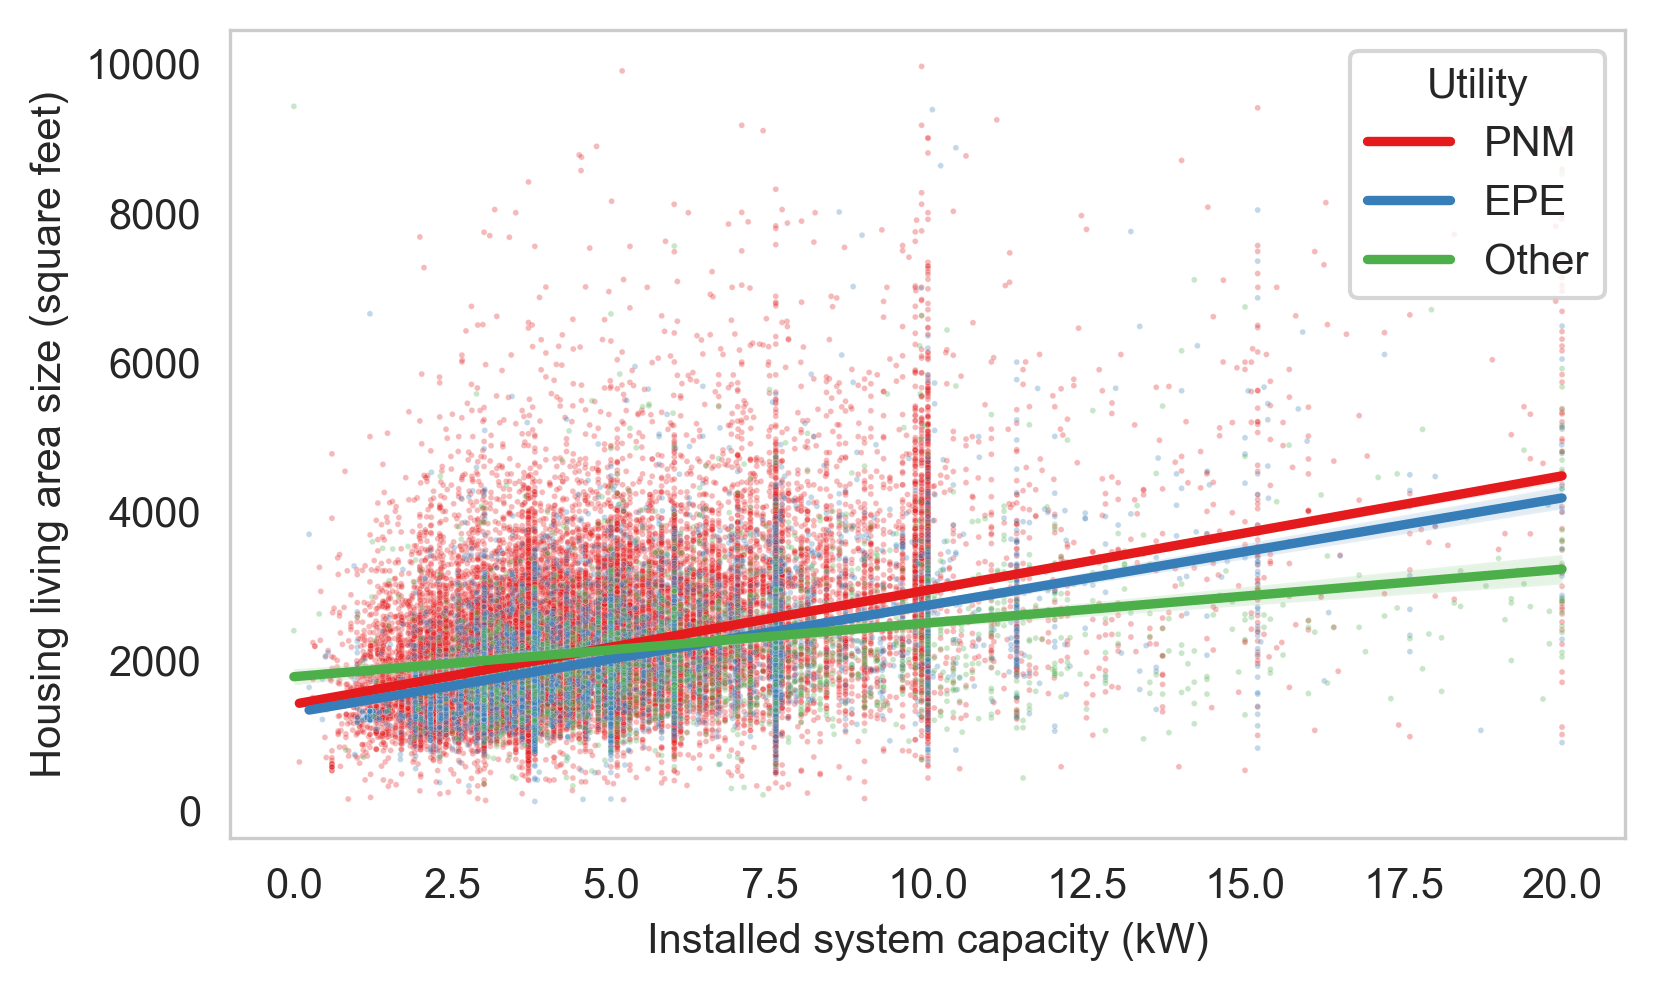
\includegraphics[width=0.9\textwidth]{figures/capacity_house_size.png}
    \caption{Linear relationship between installed capacity and housing size}
    \label{fig:capacity_size}
        \begin{flushleft}
        \footnotesize Note: Each colored dot in the graph represent on system within the corresponding utility service area. PNM stands for the Public Service Company of New Mexico, EPE stands for El Paso Electric, and Other includes all other utilities in NM.
    \end{flushleft}
\end{figure}

\autoref{fig:median_cap_map} shows the spatial distribution of median installed capacity. The map indicates that rural areas with low installation counts (\autoref{fig:installation_count}) tend to have higher median installed capacities.


\begin{figure}[!ht]
    \centering
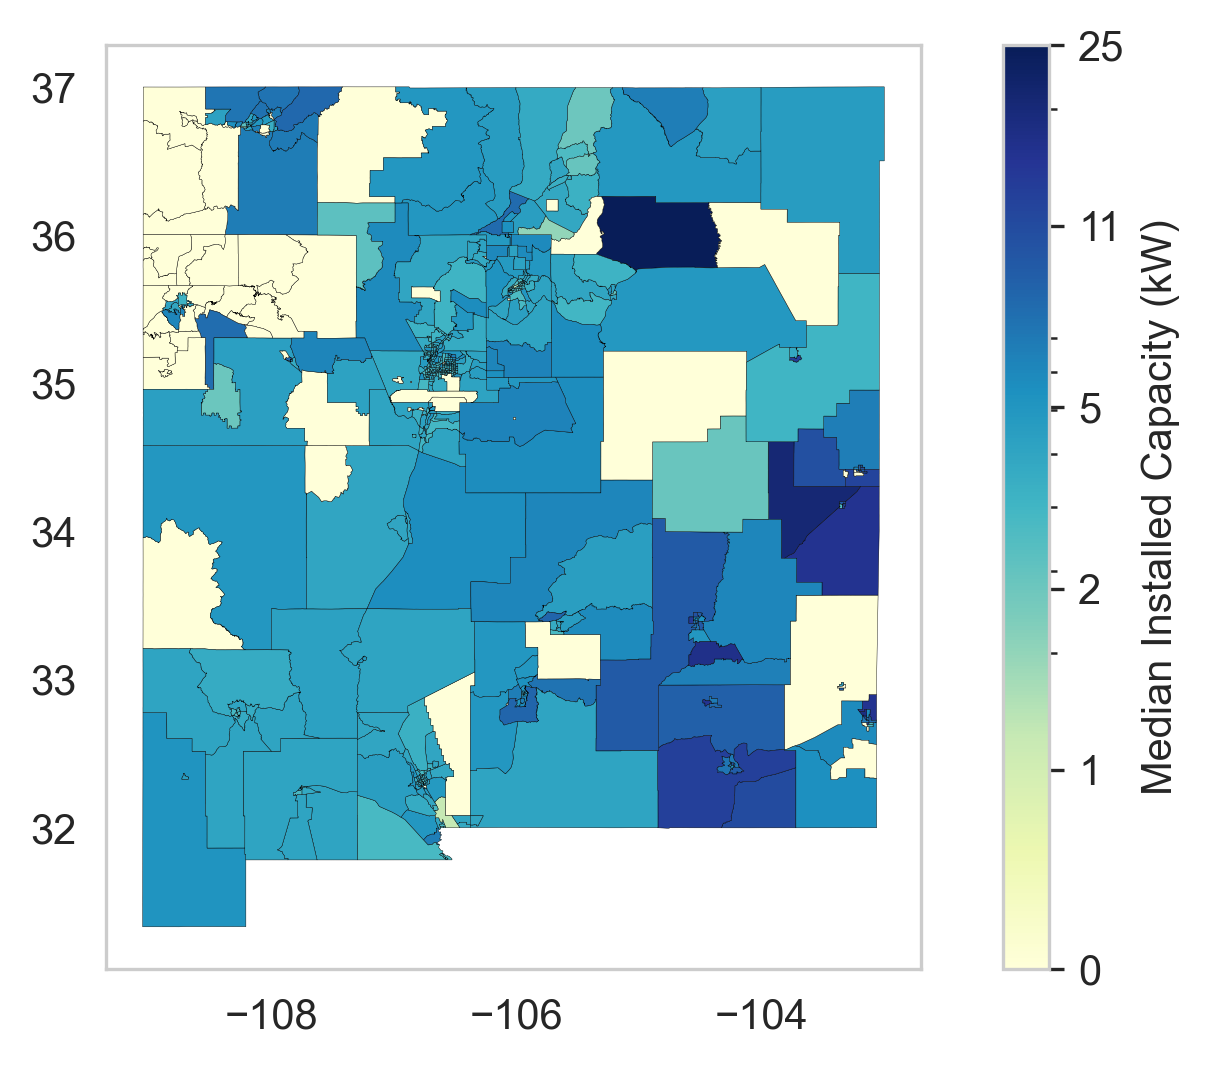
\includegraphics[width=0.65\textwidth]{figures/tract_median_capacity_map.png}
    \caption{Median system capacity by census tract}
    \label{fig:median_cap_map}
        \begin{flushleft}
        \footnotesize Note: The median system capacity for all installed systems within the census tract area. The census tracts areas are defined in the 2020 Decennial Census. The legend is in logarithm scale. 
    \end{flushleft}
\end{figure}


In summary, residential solar adoption in NM has grown exponentially since 2000, driven by decreasing solar panel costs and supportive tax incentives. However, this growth has been unevenly distributed across different geographical, income, and demographic groups. Urban areas, higher-income neighborhoods, and White-majority tracts have seen higher adoption rates compared to their rural, lower-income, and disadvantaged counterparts. The capacity of installed systems also varies, with larger systems more common in larger homes and areas with stronger utility incentives. These trends and distributions directly motivates the empirical analyses we carry out in the following sections.


%%%%%%%%%%%%%%%%%%%%%%%%%%%%%%%%%%%
\section{Adoption equity analysis}
% Section on the tract-level analysis
\label{sec:adoption_equity}

An important aspect of solar equity is the adoption equity across different demographic and socioeconomic groups. In this section, we investigate the equity of solar adoption by examining the impact of key factors on both the extensive margin (the likelihood of solar PV adoption within census tracts) and the intensive margin (the magnitude of solar PV installations). This analysis is essential for understanding how census tract characteristics influence solar adoption. Additionally, we focus on estimating the effectiveness of the state solar tax credit in promoting the equitable adoption of solar PV.

Our primary research question is: How do demographic and socioeconomic characteristics affect the likelihood and magnitude of solar PV adoption? This question is important for two reasons. First, it helps identify whether existing adoption patterns disproportionately favor certain demographic groups, potentially exacerbating social inequalities. Second, by analyzing the effectiveness of New Mexico's solar tax credit programs, SMDTC and NSMDTC, we can evaluate whether these incentives successfully mitigate disparities related to income, race, ethnicity, and education. 

\subsection{Data description}

We conduct our aggregate analysis at the 2010 census tract level. New Mexico had 499 census tracts in the 2010 Decennial Census, which increased to 612 in the 2020 Census. We normalize all data to the 2010 tract level to create a balanced panel dataset spanning from 2010 to 2022, ensuring consistency and comparability across the entire study period. The normalization method is detailed in Appendix \ref{subsec:Variable_Cal}.

The key variable we use to estimate the adoption disparities is the aggregate count of newly installed residential solar PV systems each year at the census tract level. We merge the aggregated installation data with other census tract-level variables that may impact solar adoptions, including racial composition, education level, area median income, and disadvantaged status. We include controls for housing characteristics, spatial weather patterns, electricity providers, and state credit incentives.

The dataset comprises 498 tracts in NM from 2010 through 2022 after excluding one census tract with a zero population across all study years. Table \ref{tab:datasource} provides detailed explanations of variables used in the empirical analysis and their respective data sources. 

\begin{table}[!ht]
\caption{Variable descriptions and data sources}
\centering
\label{tab:datasource}
\resizebox{0.945\textwidth}{!}{%
\begin{tabular}{lll}
\hline
Variable & Description & Data sources \\ \hline
\multicolumn{3}{l}{\textit{\textbf{Dependent variables}}} \\
Count & Installed system count & EMNRD, NMPRC, and individual utilities \\ \hline
\multicolumn{3}{l}{\textit{\textbf{Explanatory variables}}} \\
Installation price & \begin{tabular}[c]{@{}l@{}}New Mexico average installation price, \\ cent/W\end{tabular} & \begin{tabular}[c]{@{}l@{}}Lawrence Berkeley National Lab \\Tracking the Sun database \end{tabular} \\
\textbf{Housing characteristics} &  &  \\
Total housing unit & Total housing units & U.S. Census Bureau  (DP04)\\
Owner occupied & Owner occupied rate & U.S. Census Bureau (DP04) \\
Electricity & \begin{tabular}[c]{@{}l@{}}Share of of housing with electricity \\ as main the heating source\end{tabular} & U.S. Census Bureau (B25040) \\
Built year group & \begin{tabular}[c]{@{}l@{}}Median housing age year group\\ Built after 2020 = 1;\\ Built between 2010 and 2019 = 2; \\ Built between 2000 and 2009 = 3; \\ Built between 1990 and 1999 = 4; \\ Built between 1980 and 1989 = 5, \\ Built between 1970 and 1979 = 6; \\ Built between 1960 and 1969 = 7; \\ Built between 1950 and 1959 = 8; \\ Built between 1940 and 1949 = 9; \\ Built in 1939 or earlier = 10.\end{tabular} & \begin{tabular}[c]{@{}l@{}}Authors' calculation based on \\ Census Bureau (DP04) \end{tabular} \\
\textbf{Racial composition} &  &  \\
Racial diversity & Racial diversity & \begin{tabular}[c]{@{}l@{}}Authors' calculation based on \\ Census Bureau (DP05) \end{tabular}  \\
White & Share of one race White population & U.S. Census Bureau (DP05) \\
Hispanic & Share of Hispanic population & U.S. Census Bureau (DP05) \\
Non-Hispanic White & Share of Non-Hispanic White population & U.S. Census Bureau (DP05) \\
\textbf{Electricity provider variables} &  &  \\
Utility type & \begin{tabular}[c]{@{}l@{}} IOU only = 1; \\ Cooperative only = 2; \\ Public utility only = 3; \\ IOU \& Cooperative = 4; \\ IOU \& Public utility = 5; \\ Cooperative \& Public utility = 6; \\ IOU \& Cooperative \& Public \\ utility = 7\end{tabular} & \begin{tabular}[c]{@{}l@{}}Homeland Infrastructure Foundation\\ -Level Data (HIFLD)\end{tabular} \\
PNM & \begin{tabular}[c]{@{}l@{}}Dummy for PNM service area\\ Yes = 1, other = 0\end{tabular} & \begin{tabular}[c]{@{}l@{}}Public Service Company of New \\ Mexico\end{tabular} \\
Electricity price & Average electricity price (cent/kWh) & \begin{tabular}[c]{@{}l@{}}Authors' calculation based on U.S. \\ Energy Information \\ Administration\end{tabular} \\
\textbf{Weather variables} &  &  \\
Temperature & Average temperature & Solargis \\
GHI & Global Horizontal Irradiance (W/m$^2$) & Solargis \\
\textbf{Other demographic variables} &  &  \\
Bachelor & \begin{tabular}[c]{@{}l@{}}Share of population (25 years and over)\\ with bachelor's or higher degree\end{tabular} & U.S. Census Bureau (S1501)\\
Income & \begin{tabular}[c]{@{}l@{}}Area median income \\ (inflation-adjusted \$)\end{tabular} & U.S. Census Bureau (S1903) \\
Population & Total population & U.S. Census Bureau (DP05)\\
Disadvantage & Disadvantage rate & \begin{tabular}[c]{@{}l@{}}Climate and Economic Justice \\ Screening Tool\end{tabular} \\
Urban & Share of urban housing units & U.S. Census Bureau (H2)\\
Credit & \begin{tabular}[c]{@{}l@{}}Dummy for state credit incentives\\ Yes = 1, other = 0\end{tabular} & Authors' compilation \\ \hline
\multicolumn{3}{l}{\textit{Note: See Appendix \ref{subsec:Variable_Cal} for details on the author-calculated variables.}} \\
\end{tabular}%
}
\end{table}

We empirically investigate the disparity in solar PV adoptions across different demographic groups from two perspectives: 1) the impact of key factors on the extensive margin, which is the likelihood of solar PV adoption within census tracts over different years, and 2) the impact of key factors on the intensive margin, which represents the magnitude of solar PV installations. We discuss the details of our methodology and findings in the following sections.


\subsection{The extensive margin of adoption}

To estimate adoption equity on the extensive margin, we use the aggregated installation data to generate a binary dependent variable indicating the presence of any new solar installation within a census tract-year. Figure \ref{fig:stack_installation} shows the number of census tracts with solar installation in each year. In 2022, 403 census tracts had at least one installation, while 95 census tracts had no installations. This represents a substantial increase in the extensive margin compared to 2010 when 221 census tracts had at least one installation and 277 census tracts had none.

Table \ref{tab:first-stage summary stat} presents summary statistics for all variables over the sample period. We observe large standard deviations of income and housing value, indicating significant variability across the dataset and a wide financial disparity across census tract. To account for these skewed distributions, we take the logarithm of these variables in the regression analysis. 

\begin{figure}[!ht]
    \centering
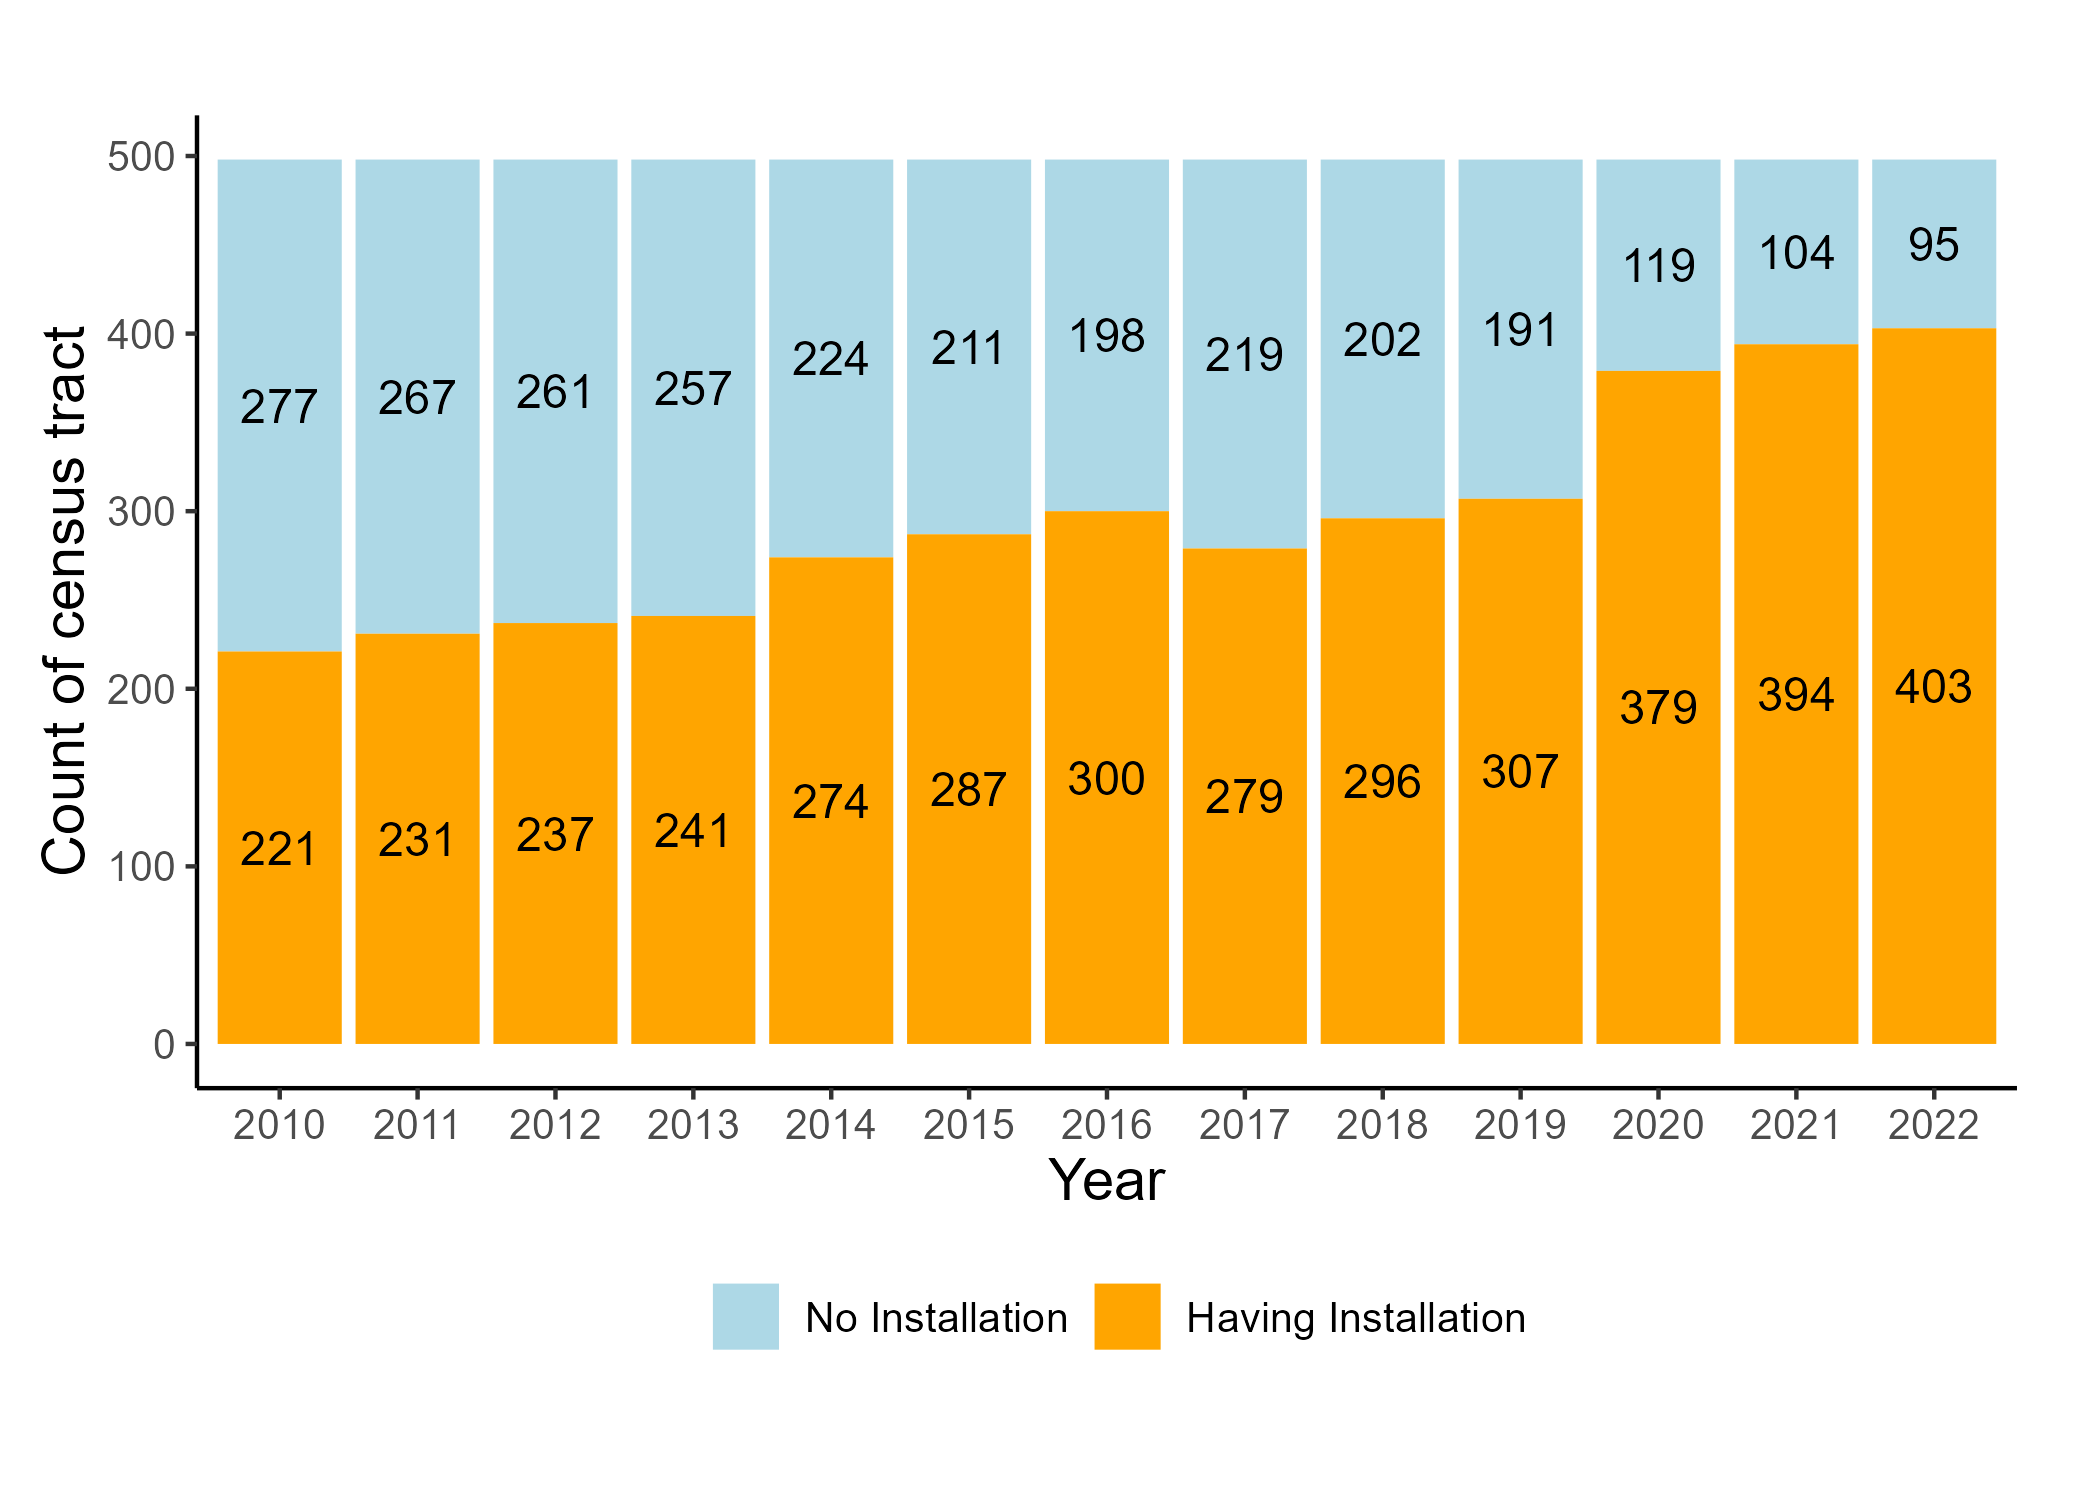
\includegraphics[width=0.9\textwidth]{figures/stack_installation.png}
    \caption{Number of census tract with/without solar installation by year}
    \label{fig:stack_installation}
\end{figure}

We compare the impact of various demographic and socioeconomic characteristics on the probability of having solar installations through a linear probability model (LPM) with county and year-fixed effects. Below is the model specification. Considering the limitations of the LPM, such as the linearity assumption, we use the fixed effect Logit model as a robustness check.


\begin{equation}\label{reg_1}
W_{it}= \alpha_{0} + \alpha_{1}H_{it} + \alpha_{2}WH_{it} + \alpha_{3}ln(INC_{it}) + \alpha_{4}EDU_{it} + \alpha_{5}DIS_{it} +\sum_{l}\gamma_{l}C_{it} + \lambda_{t} + \nu_{j} + \epsilon_{jt},
\end{equation}
where $W_{it}$ is the binary variable indicating whether there is any solar adoption within census tract $i$ in year $t$. We consider four key explanatory variables from race, ethnicity, financial, and education perspectives. Specifically, $H$ represents the share of the Hispanic population, $WH$ represents the share of the White population, $INC$ is the area median household income, $EDU$ is the share of the population with a bachelor's degree or higher, and $DIS$ is a dummy variable indicating whether a census tract in year t is disadvantaged. $C$ is the vector of control variables, which includes total population, average solar installation price, housing characteristics, and share of urban housing units. Other unobserved policies and incentives at the county level are accounted for through fixed effects. We specify $Year$ in the fixed effect as continuous to capture the trend over time.


Table \ref{tab:probability_regression} presents the model results for the extensive margin of solar adoption (full results in Table \ref{tab:probability_regression_full}). Comparing the outputs of the LPM with the logit marginal effects, we find that the LPM sufficiently captures the impact of key characteristics on the likelihood of solar adoption. There is a general increasing trend in solar adoption over the study period. The probability of new solar installation is positively correlated with the Hispanic population share, White population share, and education, although these correlations are relatively modest. Income has the highest impact on the likelihood of adoption; a 1\% increase in the area median income increases the likelihood by 12 percentage points. 

The extensive margin analysis indicates that demographic and socioeconomic factors, particularly income, significantly influence the likelihood of solar adoption. Next, we will examine the intensive margin to understand how these factors impact the scale of solar PV installations within census tracts.

\begin{table}[!ht]
\centering
\caption{Regression results for the extensive margin}
\label{tab:probability_regression}
\resizebox{0.8\textwidth}{!}{
\begin{tabular}{@{\extracolsep{2pt}}lcc}
\small
\\[-1.8ex]\hline
\hline \\[-1.8ex]
& \multicolumn{2}{c}{\textit{Dependent Variable: Having new installation}} \
\cr \cline{2-3}
\\[-1.8ex] & \multicolumn{1}{c}{Linear Probability} & \multicolumn{1}{c}{Logit Marginal Effect} \\
\hline \\[-1.8ex]
Hispanic & 0.001$^{**}$ & 0.001$^{***}$ \\
& (0.000) & (0.000) \\
White & 0.003$^{***}$ & 0.003$^{***}$ \\
& (0.000) & (0.000) \\
Log Area Median Income & 0.120$^{***}$ & 0.140$^{***}$ \\
& (0.019) & (0.018) \\
Bachelor & 0.003$^{***}$ & 0.004$^{***}$ \\
& (0.001) & (0.001) \\
Disadvantaged & 0.003 & 0.013 \\
& (0.013) & (0.012) \\
\hline \\[-1.8ex]
Control & Yes & Yes \\
Year FE & Yes & Yes \\
County FE & Yes & Yes \\
Year trend & 0.043$^{***}$ & 0.048$^{***}$ \\
\hline \\[-1.8ex]
Observations & 6,472 & 6,446 \\
R-squared & 0.522 &  \\
\hline
\hline \\[-1.8ex]
\textit{Note:} & \multicolumn{2}{r}{$^{*}$p$<$0.05; $^{**}$p$<$0.01; $^{***}$p$<$0.001} \\
    \end{tabular}}
\end{table}

\subsection{The intensive margin of adoption}

Given the spatial disparities in adoption across different census tracts, we aim to assess the extent of solar PV adoption within these tracts and identify whether certain demographic and socioeconomic groups are installing more systems by estimating adoption equity on the intensive margin. We use the count of solar installations within a census tract-year as the dependent variable. Table \ref{tab: second-stage summary stat} presents summary statistics for the main variables, conditional on having at least one installation within a tract-year over the sample period. 

The average number of residential solar PV installations per census tract-year is 10.64, with installation counts ranging from a minimum of 1 to a maximum of 155, and a standard deviation of 14.84. We aim to identify the key demographic and socioeconomic factors leading to this variability in installation count through a count model. Given the presence of over-dispersion in our dependent variable, we choose the Negative Binomial (NB) model over the Poisson model. The NB regression with county and year fixed effect model can be specified as follows:

\begin{equation}
\label{reg_2}
\begin{aligned}
\log(\mu_{it}) &= \beta_{0} + \beta_{1}H_{it} + \beta_{2}WH_{it} + \beta_{3}\log(\text{Inc}_{it}) + \beta_{4}EDU_{it} + \beta_{5}DIS_{it} + \beta_{6}CR_{it} \\
&\quad + \sum_{m}\delta_{m}C_{it} + \theta_{t} + \phi_{j} + \eta_{jt}
\end{aligned}
\end{equation}

Table \ref{tab:count_regression} displays the intensive margin of solar adoption estimation within the census tract-year. We also estimate an OLS regression for comparison with the results from the NB model (full results in \autoref{tab:count_regression_full}). The linear model yields estimates similar to the NB model, and owing to its straightforward interpretability, we use this model for the analysis. Descriptive analysis in Figures \ref{fig:installation_race} and \ref{fig:install_kpop} reveal that solar installations are concentrated in census tract with a high White population share (greater than 50\%), but decreases as White population share exceeds 80\%. To address this trend, we introduce a non-linear term into the OLS model as the third model specification. 

\begin{table}[!ht]
\caption{Regression results for the intensive margin}
\label{tab:count_regression}
\centering
\resizebox{0.9\textwidth}{!}{
\begin{tabular}{lccc}
\\[-1.8ex]\hline
\hline \\[-1.8ex]
 & \multicolumn{3}{c}{Dependent Variable: System Count} \\ \cline{2-4}
 & \multicolumn{1}{c}{(1)} & \multicolumn{1}{c}{(2)} & \multicolumn{1}{c}{(3)}  \\
 & NB Marginal Effect & OLS & OLS with non-linear term   \\ \cline{1-4}
Hispanic & 0.024** & 0.018 & 0.009 \\
 & (0.012) & (0.018) & (0.018) \\
White & -0.038 & 0.055 & 0.543** \\
 & (0.025) & (0.037) & (0.214) \\
\multicolumn{3}{l}{$(\text{White})^2$} & -0.005**  \\
 & & & (0.002)  \\
Log Area Median Income & 3.885*** & 3.373*** & 3.266*** \\
 & (0.643) & (0.837) & (0.838) \\
Bachelor & 0.103*** & 0.115*** & 0.112*** \\
 & (0.017) & (0.024) & (0.024) \\
Disadvantage & -1.829*** & -1.185** & -1.150** \\
 & (0.384) & (0.563) & (0.563) \\
Credit & 6.461*** & 7.221*** & 7.250*** \\
 & (0.608) & (0.951) & (0.951) \\
Log population & 6.780*** & 7.758*** & 7.687*** \\
\cline{1-4}
Control & Yes & Yes & Yes  \\
Year FE & Yes & Yes & Yes  \\
County FE & Yes & Yes & Yes  \\
Year & All & All & All  \\
Observations & 3,849 & 3,849 & 3,849  \\
\multicolumn{2}{l}{R-squared} & 0.45 & 0.45  \\ \cline{1-4}
\hline
\hline \\[-1.8ex]
\textit{Note:} & \multicolumn{3}{r}{$^{*}$p$<$0.05; $^{**}$p$<$0.01; $^{***}$p$<$0.001} \\
\end{tabular}}
\end{table}

The OLS estimation indicates that racial and ethnic factors are not statistically significant, suggesting that they do not play a significant role in shaping solar PV across census tracts. This result demonstrates that NM does not experience significant racial and ethnic disparities in solar adoption, contrary to what prior literature suggested \parencite{gao_solar_2022,darghouth_characterizing_2022}. While the direct impact of the White population rate is not statistically significant, Model (3) reveals a significant non-linear correlation. As the White population rate increases, the solar PV adoption grows but at a diminishing rate.


The OLS results also highlight the significant roles of income, educational attainment, disadvantage status, and credit incentive availability in solar PV adoption across census tracts. Consistent with the findings of \textcite{oshaughnessy_income-targeted_2021} and \textcite{darghouth_characterizing_2022}, areas with higher income and educational attainment are more likely to install solar PV due to greater environmental awareness and a higher capacity to invest in solar energy technologies. Conversely, disadvantaged tracts face greater barriers to adoption, exhibiting a negative effect on solar PV uptake. Additionally, our analysis finds that solar credit incentives markedly increase solar PV installations, reflecting findings in \textcite{borenstein_private_2017} on the importance of financial incentives in promoting solar energy. 


Given the significantly positive impact of income on solar installations, we further explore how this impact varies across different income brackets. Additionally, we assess the effectiveness of NM's solar tax credit incentives in reducing adoption disparities related to income. To answer these research questions, we estimate the OLS model on two subsamples: (1) divided by income quartile, and (2) divided by the availability of state solar incentives.

\subsubsection{Adoption disparity by income groups}

To assess the impact of tract-level characteristics by income bracket, we calculate the average area median income over the study period and categorize census tracts into three groups: the top income quartile, the bottom income quartile, and the middle. Table \ref{tab:count_regression_income} presents the estimation results for each group, revealing several notable observations.

First, in the bottom income quartile, none of the key demographic factors significantly impact solar installations. While the Hispanic population rate shows a positive and statistically significant effect, its overall numerical impact is small. That is, there is little disparity in solar adoption within the bottom income quartile. 

Second, in the top income quartile, the white population share negatively impacts solar installations. Specifically, a 1 percent increase in the white population correlates with an average decrease of 0.78 solar installations. This negative trend may be attributed to the non-linear effects of white population share on solar installations. As shown in Figure \ref{fig:combined_income_WH}, census tracts in the top income quartile generally have higher shares of white populations. Moreover, racial diversity has a strong positive impact on installations; areas with less racial diversity in the top quartile tend to have more installations.

Third, an intriguing trend is observed in the top income quartile’s higher sensitivity to financial factors compared to the other income groups. Contrary to expectations, income significantly boosts solar installations in this group; a 1 percent increase in area median income correlates with an additional 5.352 installations. Additionally, financial responsiveness extends to installation costs and state incentives. A one-dollar increase in the average installation price per watt results in a decrease of 4.53 installations, whereas the availability of state solar incentives contributes to an average increase of 14.55 installations. These findings suggest that households in top quartile areas exhibit high financial sensitivity when deciding on solar investments, suggesting that solar PV is a luxury good even among more affluent households.


% As expected, income positively affects solar installations across all income groups, with the strongest effect in the top quartile (5.352) and a notable impact in the middle group (4.345). However, the income effect is not significant in the bottom quartile, likely due to the low income variation within this group, which diminishes its influence on solar adoption. Moreover, households in the bottom quartile face a larger financial burden, making small income increases insufficient to significantly promote solar adoption. 

% We also find that the rate of Hispanic population has a positive and significant effect in the bottom and top income quartiles, suggests that solar adoption among Hispanic communities is more pronounced in the lowest and highest income groups. However, the overall impact is relatively minor from a numerical standpoint, suggesting that changes in Hispanic population rate do not significantly influence solar adoption counts. On the other hand, the White population rate shows a significant negative effect in the top income quartile, indicating a 1.3\% increase in the White population correlates with an average decrease of 1 solar installation (a 1\% increase in the White population correlates with an average decrease of 0.78 solar installations). From the frequency of White population rate within top income quartile shown in Figure \ref{fig:combined_income_WH}, areas with higher median income tend to have higher proportions of the White population. Then, this negative effect in the top income quartile reinforces the finding that wealthier areas with higher White population percentages experience diminishing rates of solar PV adoption.

\begin{figure}[!ht]
    \centering
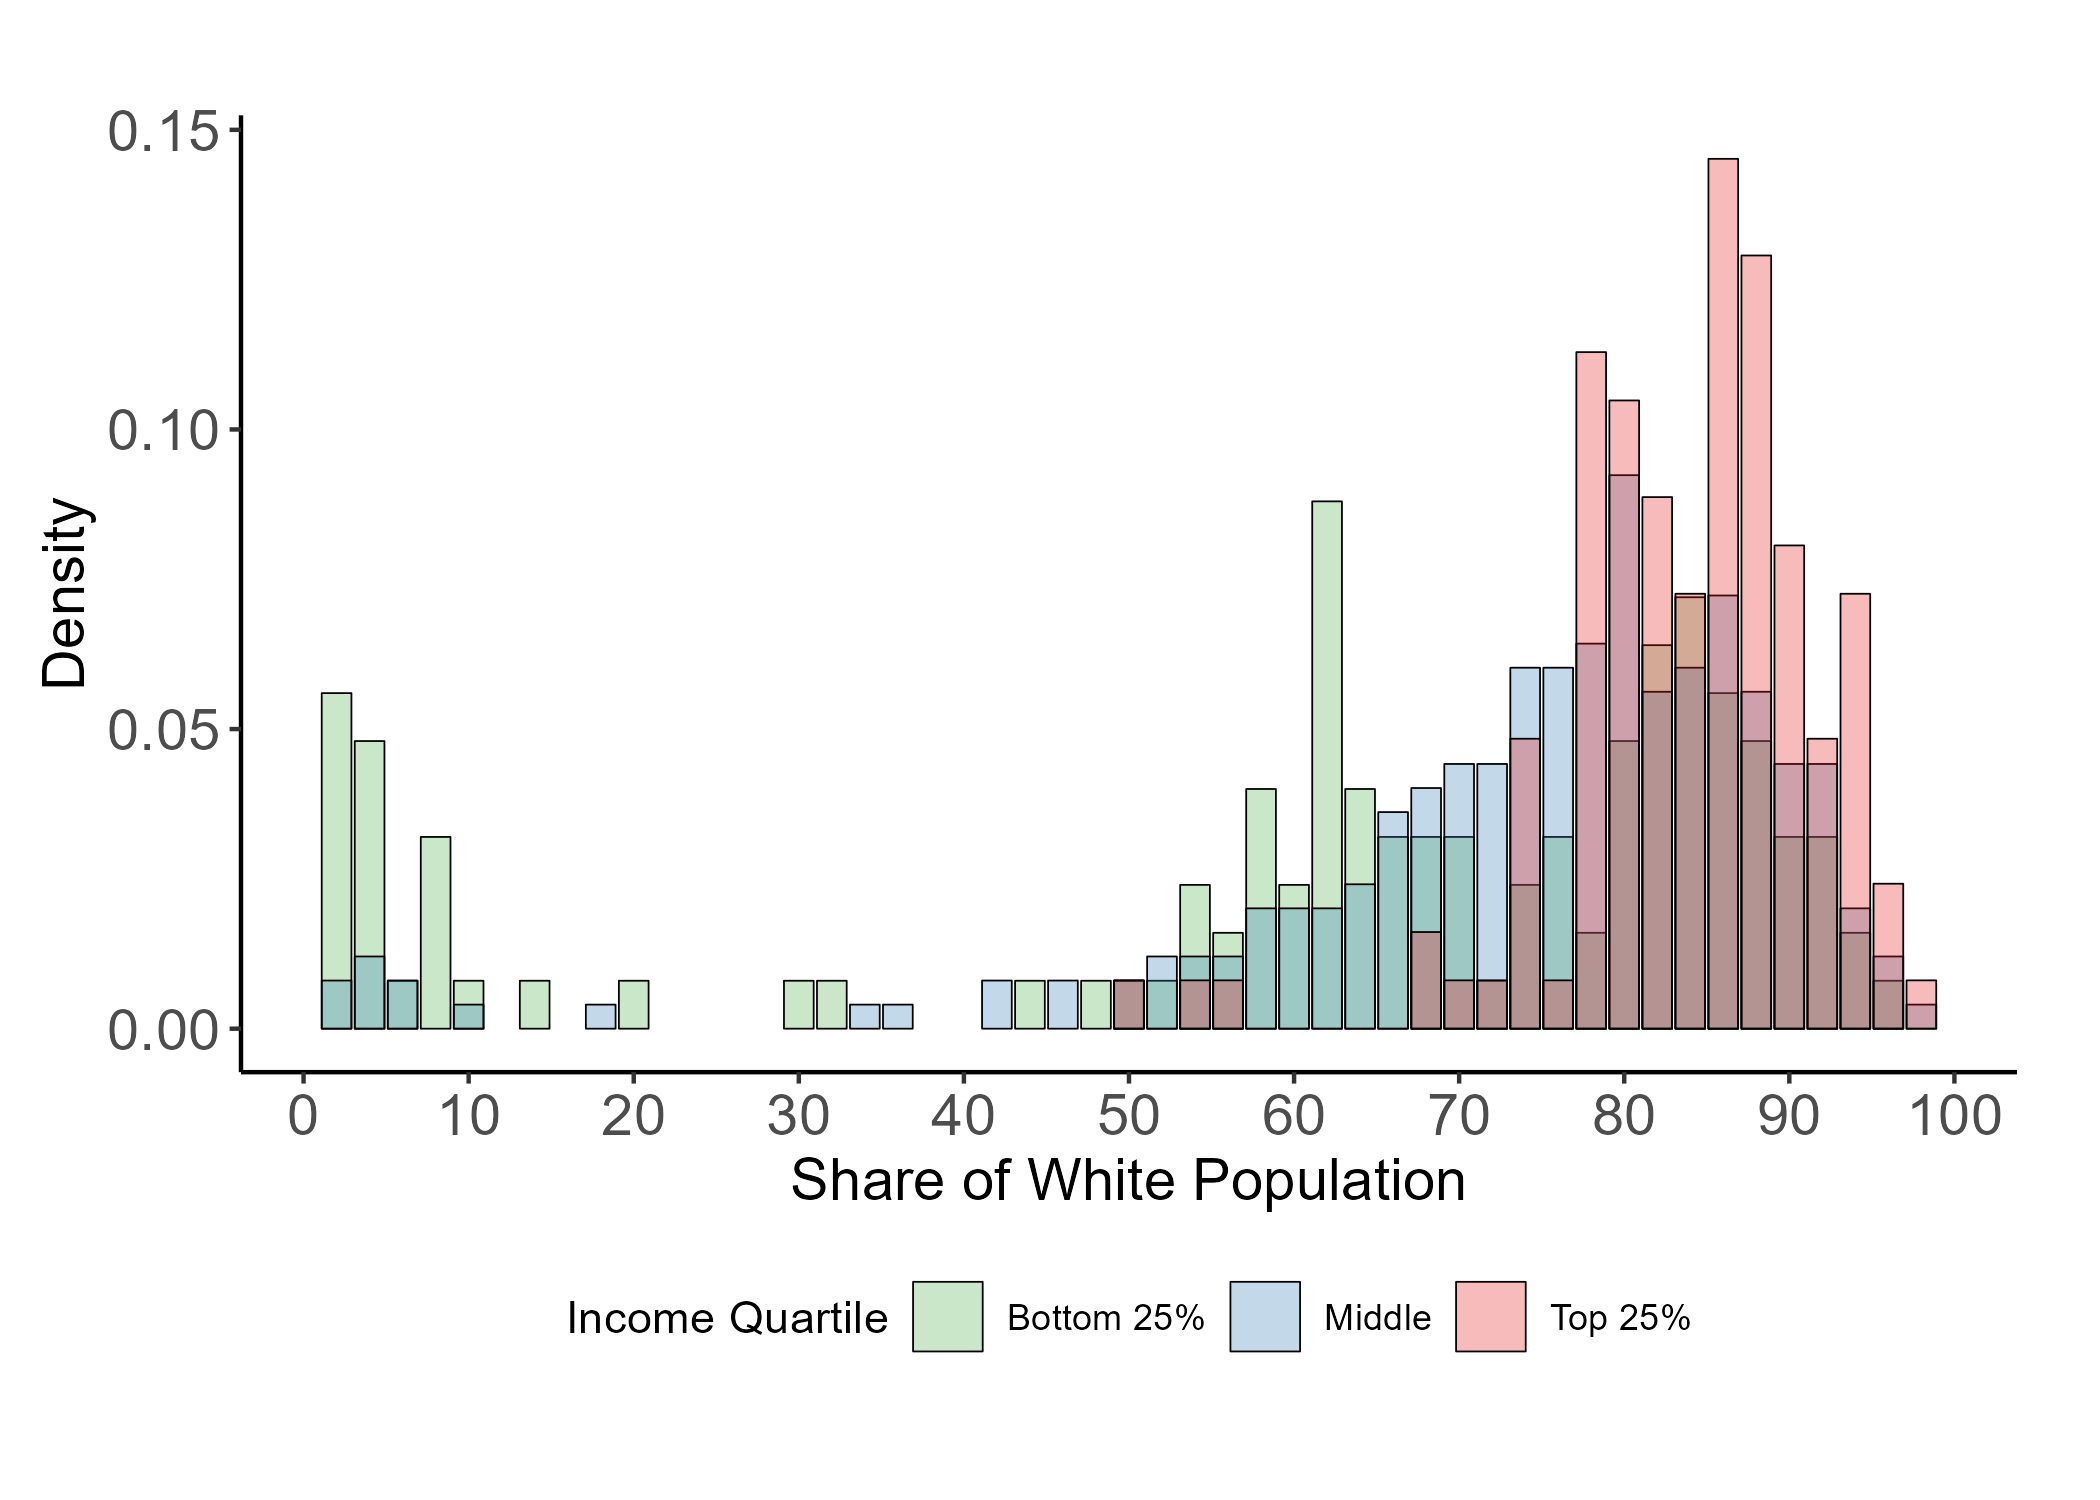
\includegraphics[width=0.9\textwidth]{figures/combined_income_WH.png}
    \caption{White population rate in census tracts by income quartile}
    \label{fig:combined_income_WH}
     \begin{flushleft}
        \footnotesize Note: The income quartile classification is based on the average census tract area median income from 2010 to 2022. The share of White population in each census tract is the average of White population rate from 2010 to 2022. 
    \end{flushleft}
\end{figure}

% Educational attainment also significantly increases solar adoption in the top income quartile and middle income group, but not in the bottom quartile. Regarding the lack of significance in the bottom quartile, several factors could contribute to this result. Firstly, there is a high correlation of 0.69 between education and income (shown in Figure \ref{fig:corr_matrix}). Income may capture most of the variation in solar adoption behavior in the low-income areas. Secondly, the presence of an information barrier could be another factor. Low-income areas may face challenges in accessing information about solar adoption and relative policies, leading to fewer adoptions despite potentially favorable educational backgrounds.

% The result reveals that top income quartile areas are more sensitive to financial factors such as installation price and state solar incentives compared to other income groups. Specifically, a one-cent increase in the average installation price per watt correlates to a decrease of 5 solar installations in the top income quartile, while other income brackets experience a smaller reduction of 3 installations on average. Similarly, the availability of state solar incentives leads to an increase of 15 solar installations in the top income quartile, while middle brackets and bottom quartile only experience a 5-unit increase and 3-unit increase respectively. This suggests that households in higher-income areas may be more price-sensitive when making decisions on renewable energy investments.

%%%%%%%%%%%%%
\subsubsection{Effectiveness of the state solar tax credit}

To evaluate whether state-level solar incentives alleviate or exacerbate disparities, we divide the observations into three groups based on the availability of solar incentives. The first group includes data from 2010 to 2016 when the initial solar tax credit, SMDTC, was available. The second group comprises data from 2017 to 2019 when state-level solar incentives were absent. The last group spans from 2020 to 2022, when the New Solar Market Development Tax Credit (NSMDTC) was reintroduced. Table \ref{tab:count_regression_3 periods} shows the estimation results for each period. We analyze the effects of the state solar tax credit on adoption disparities by race and income separately.


Our findings indicate that in NM, state solar credits significantly mitigate racial disparities in solar adoption. When state incentives were available, no significant racial disparities were observed. In contrast, during periods without these incentives, a 1 percentage point increase in the White population correlated with an average increase of 0.3 solar installations, suggesting that areas with higher White population share were more likely to adopt solar technology. This pattern underscores the effectiveness of state incentives to help create a more equitable environment for solar adoption across different racial groups. 

Further analysis of income’s influence on solar adoption highlights a significant trend: during the years without state incentives (2017-2019), the correlation between income and solar installation counts was notably strong, as indicated by a coefficient of 9.787, pointing to increased income-related disparities. However, with the reintroduction of the NSMDTC in 2020, this impact significantly diminished, with the income coefficient turning negative (-0.728). This reversal suggests that the state tax credits have effectively reduced income-based disparities. 

Nonetheless, when examining the income subsample regression (\autoref{tab:count_regression_income}), it becomes evident that while the top income quartile is highly responsive to the state tax credit, the bottom quartile is not. This discrepancy may be due to the non-refundable nature of the tax credit. Therefore, those in the bottom income quartile with insufficient tax liability cannot benefit from it. Consequently, while the state tax credit reduces within-group disparity among income quartiles, it does not substantially narrow the gap across groups, diverging from the effects suggested by \textcite{oshaughnessy_rooftop_2022}. This outcome underscores the importance of incentive design in achieving equitable benefits across different income levels, as highlighted by \textcite{borenstein_distributional_2016}.

% On the other hand, while individuals with higher educational attainment were generally more likely to adopt solar technology in the early stages, this trend has weakened with the widespread adoption of solar energy. The state-level incentives did not significantly affect educational disparities. The coefficients in 2017-2019 and 2020-2022 are positive but not significant, suggesting that potential information barriers may still exist but have been alleviated by some other unobserved interventions over the years. There has been some progress in making solar technology more accessible across different educational levels in New Mexico.



%%%%%%%%%%%%%%%%%%%%%%%%%%%%%%%%%%%

\section{Distributional equity analysis}
% Section on credit claim

Another important aspect of solar equity is distributional equity, which pertains to whether the benefits of clean energy incentives are uniformly distributed across different demographic groups. In this section, we focus on the distributional equity of the state solar tax credit programs, SMDTC and NSMDTC, as they are the most prominent and salient forms of financial incentives for households. Given that solar tax credits are financed through tax dollars, understanding their distributional effects and potential regressivity is crucial for evaluating the effectiveness of these policies. Furthermore, the main motivation for solar tax credits is to promote solar adoption by reducing the financial burdens on households and to facilitate energy transition. Since the electricity produced by residential solar panels crowds out kWh for kWh of electricity from other generation sources in the grid regardless of the location and household characteristics (unless off-grid), having only a subset of households benefiting from the credit can be considered inequitable.

Our main research question is: Conditional on adopting solar, how do household and tract-level characteristics affect the probability of receiving state tax credits? Studying this question is crucial for several reasons. Firstly, it helps identify whether existing policies inadvertently favor certain demographic groups over others, which can exacerbate social inequalities. If solar incentives disproportionately benefit higher-income households or specific racial or ethnic groups, it indicates a need to redesign these policies to be more inclusive and equitable. Secondly, by understanding the factors that influence the distribution of these incentives, policymakers can develop targeted strategies to enhance the accessibility of solar energy for underrepresented and disadvantaged communities, contributing to a more just and sustainable energy transition. Lastly, evaluating the regressivity of solar tax credits ensures that public funds are used efficiently and equitably, promoting broader societal support for clean energy initiatives. Overall, this research provides valuable insights into designing more equitable and effective solar incentive programs.

We would like to note a few details about the state solar tax credit in New Mexico. First, the tax credit is 10\% of the total installation cost, with a cap of \$9,000 in the first period and \$6,000 in the second. Second, the tax credit can only be approved if the household applies for it (obviously), and approval for the tax credit requires an extensive set of documents from installers, utilities, permitting agencies, county assessors, and homeowners. Third, a household only qualifies for the tax credit if the system is owned and not leased. These specific incentive structures may also affect which types of households eventually receive the credit.

Our main hypotheses to be tested given the incentive structure are the following:
\begin{itemize}
    \item[\textbf{H1}] Households with more expensive systems, reflected by higher installed capacity, are more likely to claim the tax credit. This is because, with the flat 10\% credit, systems with a higher price tag can receive a higher absolute return.
    \item[\textbf{H2}] Less wealthy families are more likely to claim the tax credit as they have a higher marginal utility of wealth. Since we do not observe income or wealth at the household level, we use housing value as a proxy.
    \item[\textbf{H3}] Households in census tracts with higher education levels are more likely to claim credits as the application process may pose information barriers.
\end{itemize}

\subsection{Data and descriptive analysis}

We use the system-level data described in section \ref{section:data_collect} for the years when tax credits were available (2006-2016 and after 2020). Since the demographics data spans from 2010 to 2022, we restrict our sample to the overlapping years: 2010-2016 and 2020-2022. 

\autoref{fig:credit_claim} shows the number of newly installed systems each year that received or did not receive solar tax credits within PNM, EPE, SEC, and LADPU service areas. It also shows the total credit amount claimed each year by all residential solar systems. During the first phase of the tax credit program (SMDTC), the majority of installations benefited from the 10\% credit. In contrast, in the second phase (NSMDTC), more than half of the installations did not receive the credit. This gap can partially be explained by the annual funding cap implemented with NSMDTC. In 2020 and 2021, the cap was \$8 million, increasing to \$12 million in 2022 and 2023.\footnote{In 2024, Governor Lujan Grisham signed House Bill 252 into law to raise the annual aggregate cap to \$30 million per year \parencite{newsolarcap}.} The aggregate cap was reached in 2021 and 2022, resulting in 190 and 226 tax credit application rejections, respectively. Only 1\% and 3\% of the applications exceeded the individual system cap in the first and second periods, respectively.

\begin{figure}[!ht]
    \centering
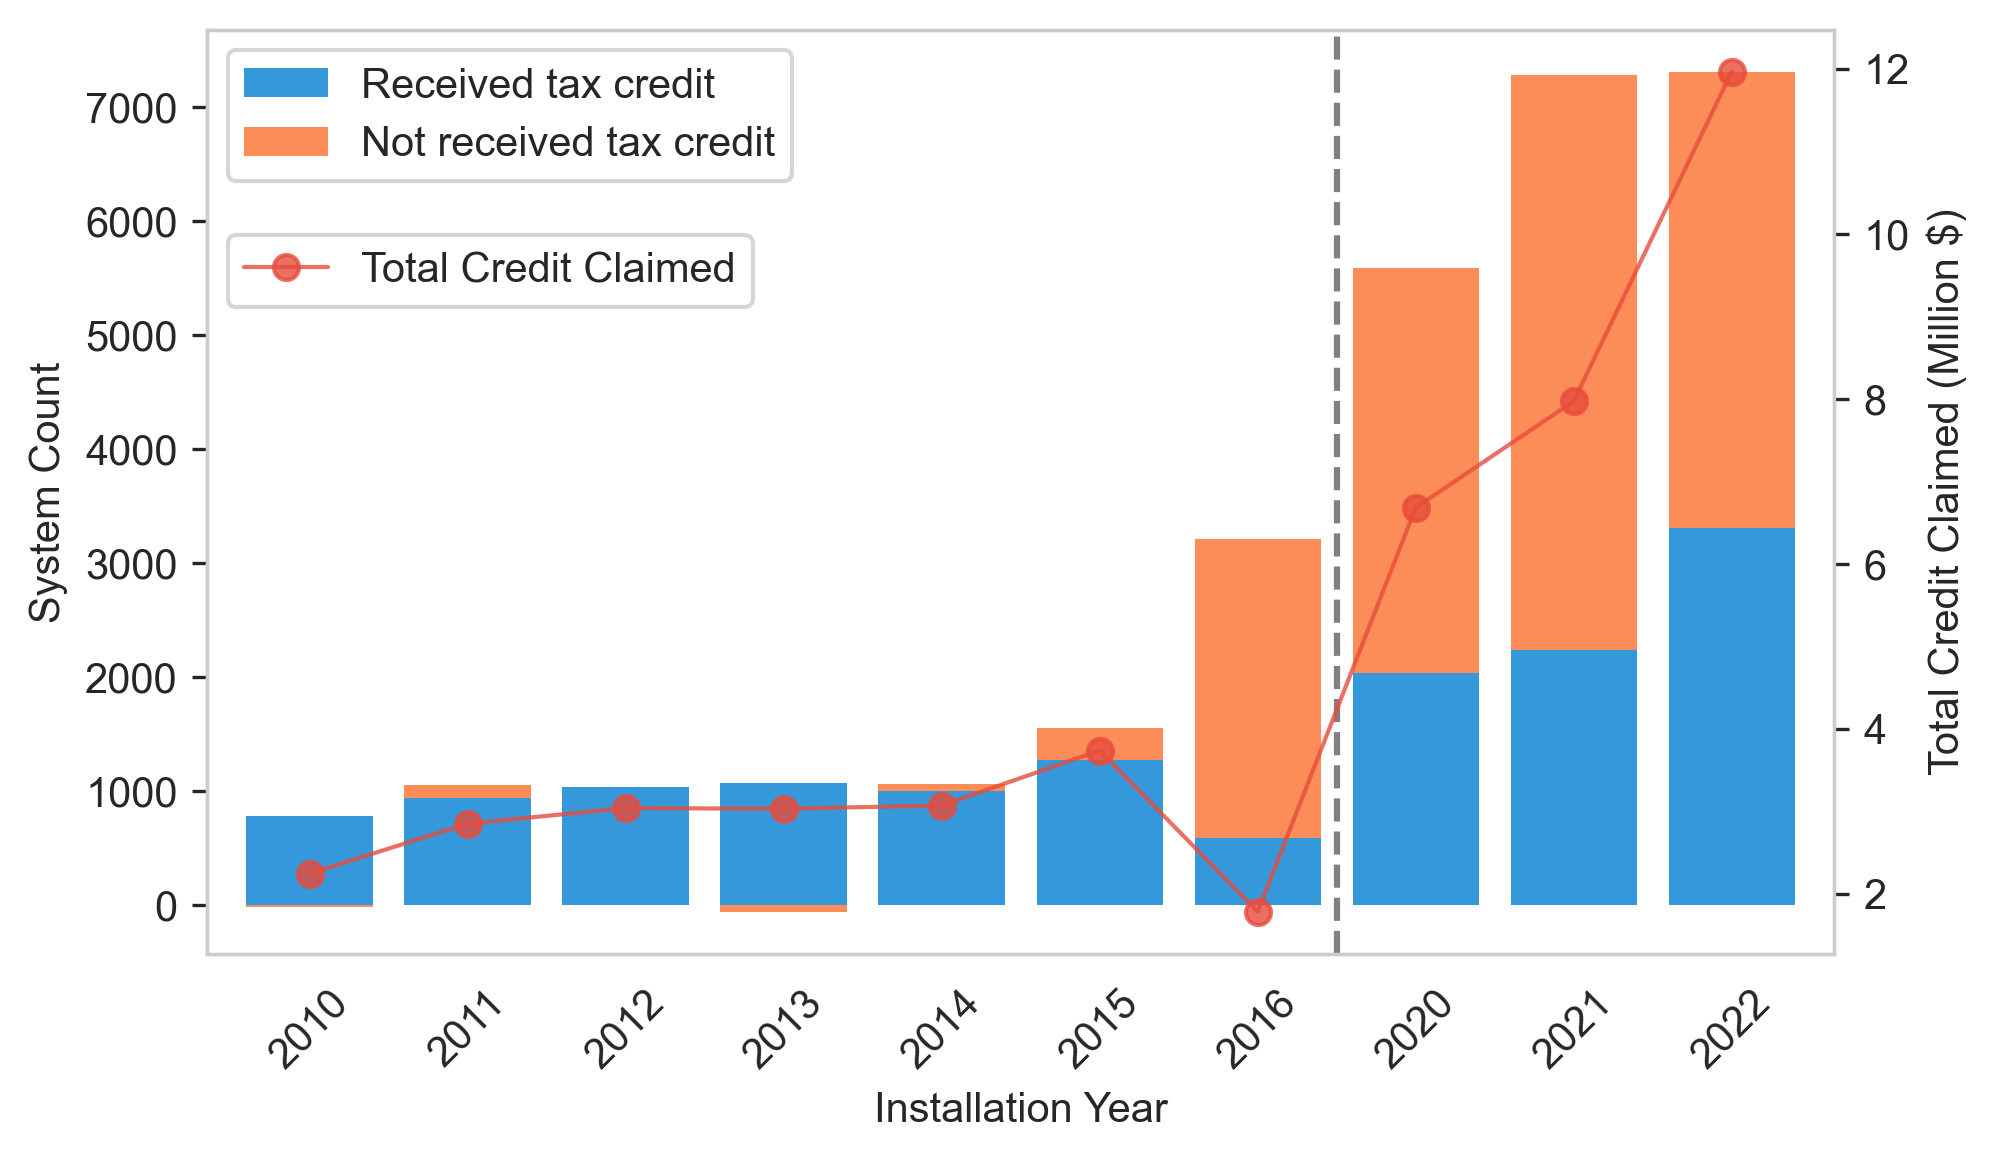
\includegraphics[width=0.9\textwidth]{figures/credit_claim.png}
    \caption{Installed systems by credit claim status and total credit claimed between 2010 and 2022}
    \label{fig:credit_claim}
      \begin{flushleft}
        \footnotesize Note: The total system counts only include systems within PNM, EPE, SEC, and LADPU service areas. The number of systems receiving credits is also for this subset of utilities only. The total credit claimed accounts for all residential systems. In 2010 and 2013, the number of systems that did not receive tax credits (orange bars) was negative. This could be due to data errors between different data sources or credit claim delays.
    \end{flushleft}
\end{figure}

\autoref{fig:credit_map} illustrates the concentration of total tax credit claims and the average amount claimed per system. Total credits concentrate in census tracts with high solar installations (\autoref{fig:tract_map}). In contrast, the average tax credit is highly correlated with the median installed capacity of the tract (\autoref{fig:median_cap_map}). 

\begin{figure}[!ht]
    \centering
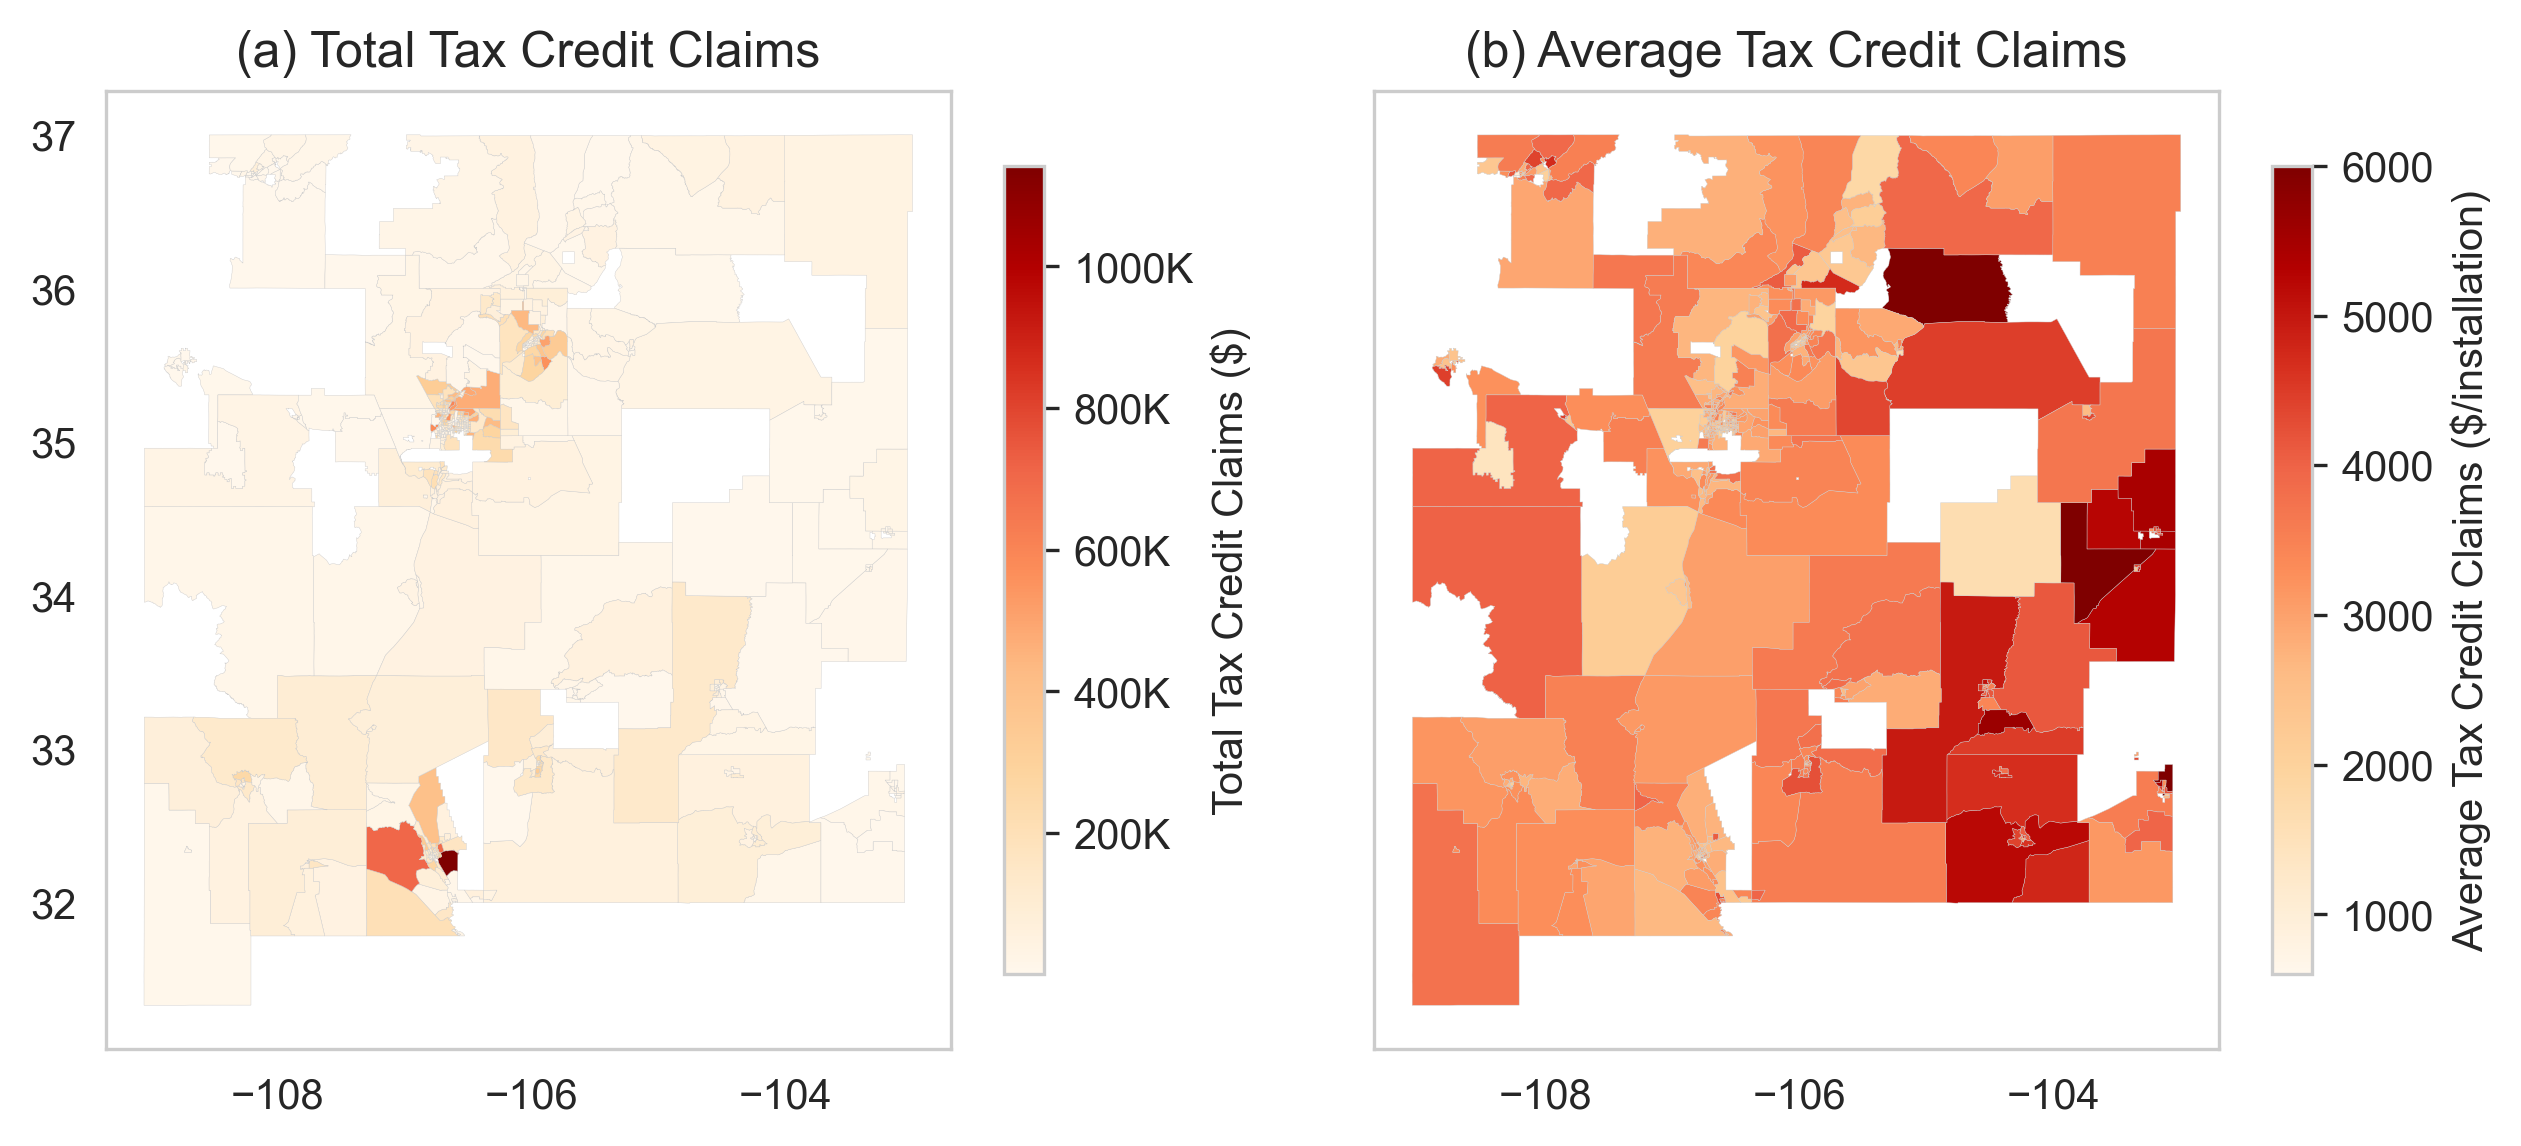
\includegraphics[width=1\textwidth]{figures/credit_claim_maps.png}
    \caption{Total and average tax credit claim by census tract}
    \label{fig:credit_map}
      \begin{flushleft}
        \footnotesize Note: The total credit claimed sums up all historical amounts of credit received in the census tract by 2022. The average credit claim uses the total amount divided by the number of systems that received tax credits.
    \end{flushleft}
\end{figure}

To answer the research question, we need to match the two data sources of solar installations to identify which systems received solar credits. The EMNRD data contains a wealth of information but only for systems that received tax credits, while the utility data includes the universe of all systems installed. We match the recorded address of the installed systems. Since the recorded address for the same system may vary across datasets, some of the systems in the EMNRD data cannot be found in the utility dataset despite our best efforts. \autoref{tab:compare_emnrd_utility} shows the result of the matching, which, although imperfect, remains statistically insignificant. We also dropped any households with living areas of less than 100 square feet to avoid extreme outliers. The resulting dataset includes 26,735 unique systems.


\autoref{tab:sumstat} shows the summary statistics of the matched dataset, and \autoref{fig:corr_matrix} displays the correlation matrix of the key variables.




\subsection{The extensive margin of tax credit claim}

The dependent variable in our analysis is whether a household received a tax credit upon adopting solar energy. We use the linear probability model (LPM) as a preliminary step to decompose the effect of various household and tract-level characteristics on the probability of claiming credit. We run the logit model as a robustness check. The model is specified as follows:

\begin{equation}\label{reg_3}
    \text{SolarTaxCredit}_{hlt} = \alpha + \beta_1 X_{ht} + \beta_2 C_{lt}  + \gamma_t +  \delta_c + \theta_u + \varepsilon_{lt},
\end{equation}
where $\text{SolarTaxCredit}_{hlt}$ is a binary variable indicating whether household $h$ in census tract $l$ received a solar tax credit in year $t$, $X_{ht}$ is a vector of household-level variables for household $h$ in year $t$, $C_{lt}$ is a vector of census tract-level variables for the census tract $l$ in year $t$, $\gamma_t$ is the year fixed effect, $\delta_c$ is the county fixed effect, $\theta_u$ is the utility fixed effect, standard errors are clustered at the census tract level.

We test five model variations: (1) including only household-level variables, (2) including both household- and census tract-level variables, (3) with year fixed effects, (4) with year and utility fixed effects, and (5) with year and county fixed effects.

Model (1) examines how household-level characteristics alone affect the probability of claiming the credit. Model (2) examines whether the tax credit benefits concentrate in communities with certain demographic characteristics. Model (3) controls for time-varying unobserved factors, such as changes in solar PV price trends and societal awareness and acceptance of solar PV. Model (4) controls for time-invariant utility-specific characteristics, including utility type (IOU, coop, or public utility), solar incentives, and infrastructure. Model (5) controls for county-specific characteristics, including regulatory environment and geographic factors not captured by the demographic controls. The results of these models are presented in \autoref{tab:credit_claim_full_regression}. The regression result of the logit model with the same model specifications is reported in \autoref{tab:reg_logit}.


\begin{table}[!ht] \centering
  \caption{Regression results on state credit claim}
  \label{tab:credit_claim_full_regression}
  \resizebox{1\textwidth}{!}{
\begin{tabular}{@{\extracolsep{5pt}}lccccc}
\\[-1.8ex]\hline
\hline \\[-1.8ex]
& \multicolumn{5}{c}{\textit{Dependent variable: State Credit}} \
\cr \cline{2-6}
\\[-1.8ex] & (1) & (2) & (3) & (4) & (5) \\
\hline \\[-1.8ex]
 System capacity & -0.005$^{***}$ & 0.003$^{*}$ & 0.010$^{***}$ & 0.009$^{***}$ & 0.008$^{***}$ \\
& (0.001) & (0.001) & (0.001) & (0.001) & (0.001) \\
 Log Zestimate & 0.294$^{***}$ & 0.148$^{***}$ & 0.117$^{***}$ & 0.134$^{***}$ & 0.156$^{***}$ \\
& (0.009) & (0.012) & (0.011) & (0.012) & (0.015) \\
 Year built & -0.002$^{***}$ & -0.000$^{}$ & -0.001$^{***}$ & -0.001$^{***}$ & -0.001$^{***}$ \\
& (0.000) & (0.000) & (0.000) & (0.000) & (0.000) \\
 Log Housing size (sq ft) & 0.047$^{***}$ & 0.029$^{*}$ & 0.004$^{}$ & -0.005$^{}$ & -0.016$^{}$ \\
& (0.014) & (0.014) & (0.013) & (0.013) & (0.015) \\
 \# of Bedrooms & -0.036$^{***}$ & -0.017$^{***}$ & -0.009$^{*}$ & -0.010$^{*}$ & -0.010$^{*}$ \\
& (0.005) & (0.005) & (0.004) & (0.004) & (0.004) \\
 \% population with bachelor degree ($>$25) & & 0.183$^{***}$ & 0.260$^{***}$ & 0.213$^{***}$ & 0.187$^{***}$ \\
& & (0.033) & (0.031) & (0.034) & (0.037) \\
 Owner occupancy rate & & -0.383$^{***}$ & 0.141$^{***}$ & 0.136$^{***}$ & 0.139$^{***}$ \\
& & (0.021) & (0.025) & (0.025) & (0.025) \\
 Mortgage rate & & -0.298$^{***}$ & -0.287$^{***}$ & -0.272$^{***}$ & -0.228$^{***}$ \\
& & (0.031) & (0.030) & (0.031) & (0.031) \\
 Log Area Median Income & & 0.067$^{***}$ & -0.015$^{}$ & -0.005$^{}$ & -0.005$^{}$ \\
& & (0.014) & (0.014) & (0.014) & (0.014) \\
 Log Population & & 0.054$^{***}$ & 0.016$^{*}$ & 0.015$^{*}$ & 0.024$^{**}$ \\
& & (0.007) & (0.007) & (0.007) & (0.007) \\
 Log Median Age & & 0.048$^{*}$ & 0.009$^{}$ & 0.008$^{}$ & 0.023$^{}$ \\
& & (0.022) & (0.021) & (0.021) & (0.021) \\
 \% population identified as White & & 0.064$^{}$ & 0.017$^{}$ & -0.011$^{}$ & -0.067$^{}$ \\
& & (0.038) & (0.036) & (0.038) & (0.040) \\
 \% population identified as Hispanic & & -0.090$^{***}$ & -0.105$^{***}$ & -0.145$^{***}$ & -0.142$^{***}$ \\
& & (0.024) & (0.023) & (0.025) & (0.029) \\
 Urban share & & -0.061$^{***}$ & -0.031$^{**}$ & -0.021$^{}$ & -0.008$^{}$ \\
& & (0.012) & (0.011) & (0.012) & (0.012) \\
 Within disadvantaged census tracts & & -0.039$^{***}$ & -0.034$^{***}$ & -0.032$^{***}$ & -0.042$^{***}$ \\
& & (0.009) & (0.009) & (0.009) & (0.009) \\
 Year Fixed Effects & No & No & Yes & Yes & Yes \\
 Utility Fixed Effects & No & No & No & Yes & No \\
 County Fixed Effects & No & No & No & No & Yes \\
\hline \\[-1.8ex]
 Observations & 25234 & 25234 & 25234 & 25234 & 25234 \\
 $R^2$ & 0.086 & 0.157 & 0.232 & 0.233 & 0.235 \\
 Adjusted $R^2$ & 0.086 & 0.156 & 0.231 & 0.232 & 0.234 \\
 Residual Std. Error & 0.475 & 0.456 & 0.435 & 0.435 & 0.435 \\
 F Statistic & 476.601$^{***}$ & 313.067$^{***}$ & 317.205$^{***}$ & 282.905$^{***}$ & 209.254$^{***}$ \\
\hline
\hline \\[-1.8ex]
\textit{Note:} & \multicolumn{5}{r}{$^{*}$p$<$0.05; $^{**}$p$<$0.01; $^{***}$p$<$0.001} \\
\multicolumn{6}{r}\textit{Standard errors are clustered at the census tract level and are robust} \\
\end{tabular}
}
\end{table}

The results suggest that households with higher system capacity, higher housing values, and older residences are more likely to obtain tax credits. Housing value has the most significant positive impact: a 1 percent increase in housing value increases the probability of claiming the credit by 15.6 percentage points, contrary to our initial hypothesis. Additionally, households in census tracts with higher education levels, higher owner-occupancy rates, lower mortgage rates, and higher Hispanic populations are more likely to receive tax credits. Conversely, disadvantaged census tracts have fewer tax credit claims.

These results provide evidence that tax credits are concentrated among wealthier households, all else being equal, similar to findings in the literature related to other green energy incentive programs \parencite{borenstein_distributional_2016}. \autoref{fig:credit_by_zestimate_quintile} illustrates that the rate of credit claims increases for higher housing value quintiles, with more than 65\% of households in the top quintile claiming the credit, compared to only around 25\% in the bottom quintile. 

The results also suggest potential information barriers to ethnic minorities and populations with lower education levels in the tax credit program. The negative and significant coefficient for the mortgage rate suggests that more solar systems may be under leasing contracts in these census tracts, which do not qualify for the tax credits.

\begin{figure}[!ht]
    \centering
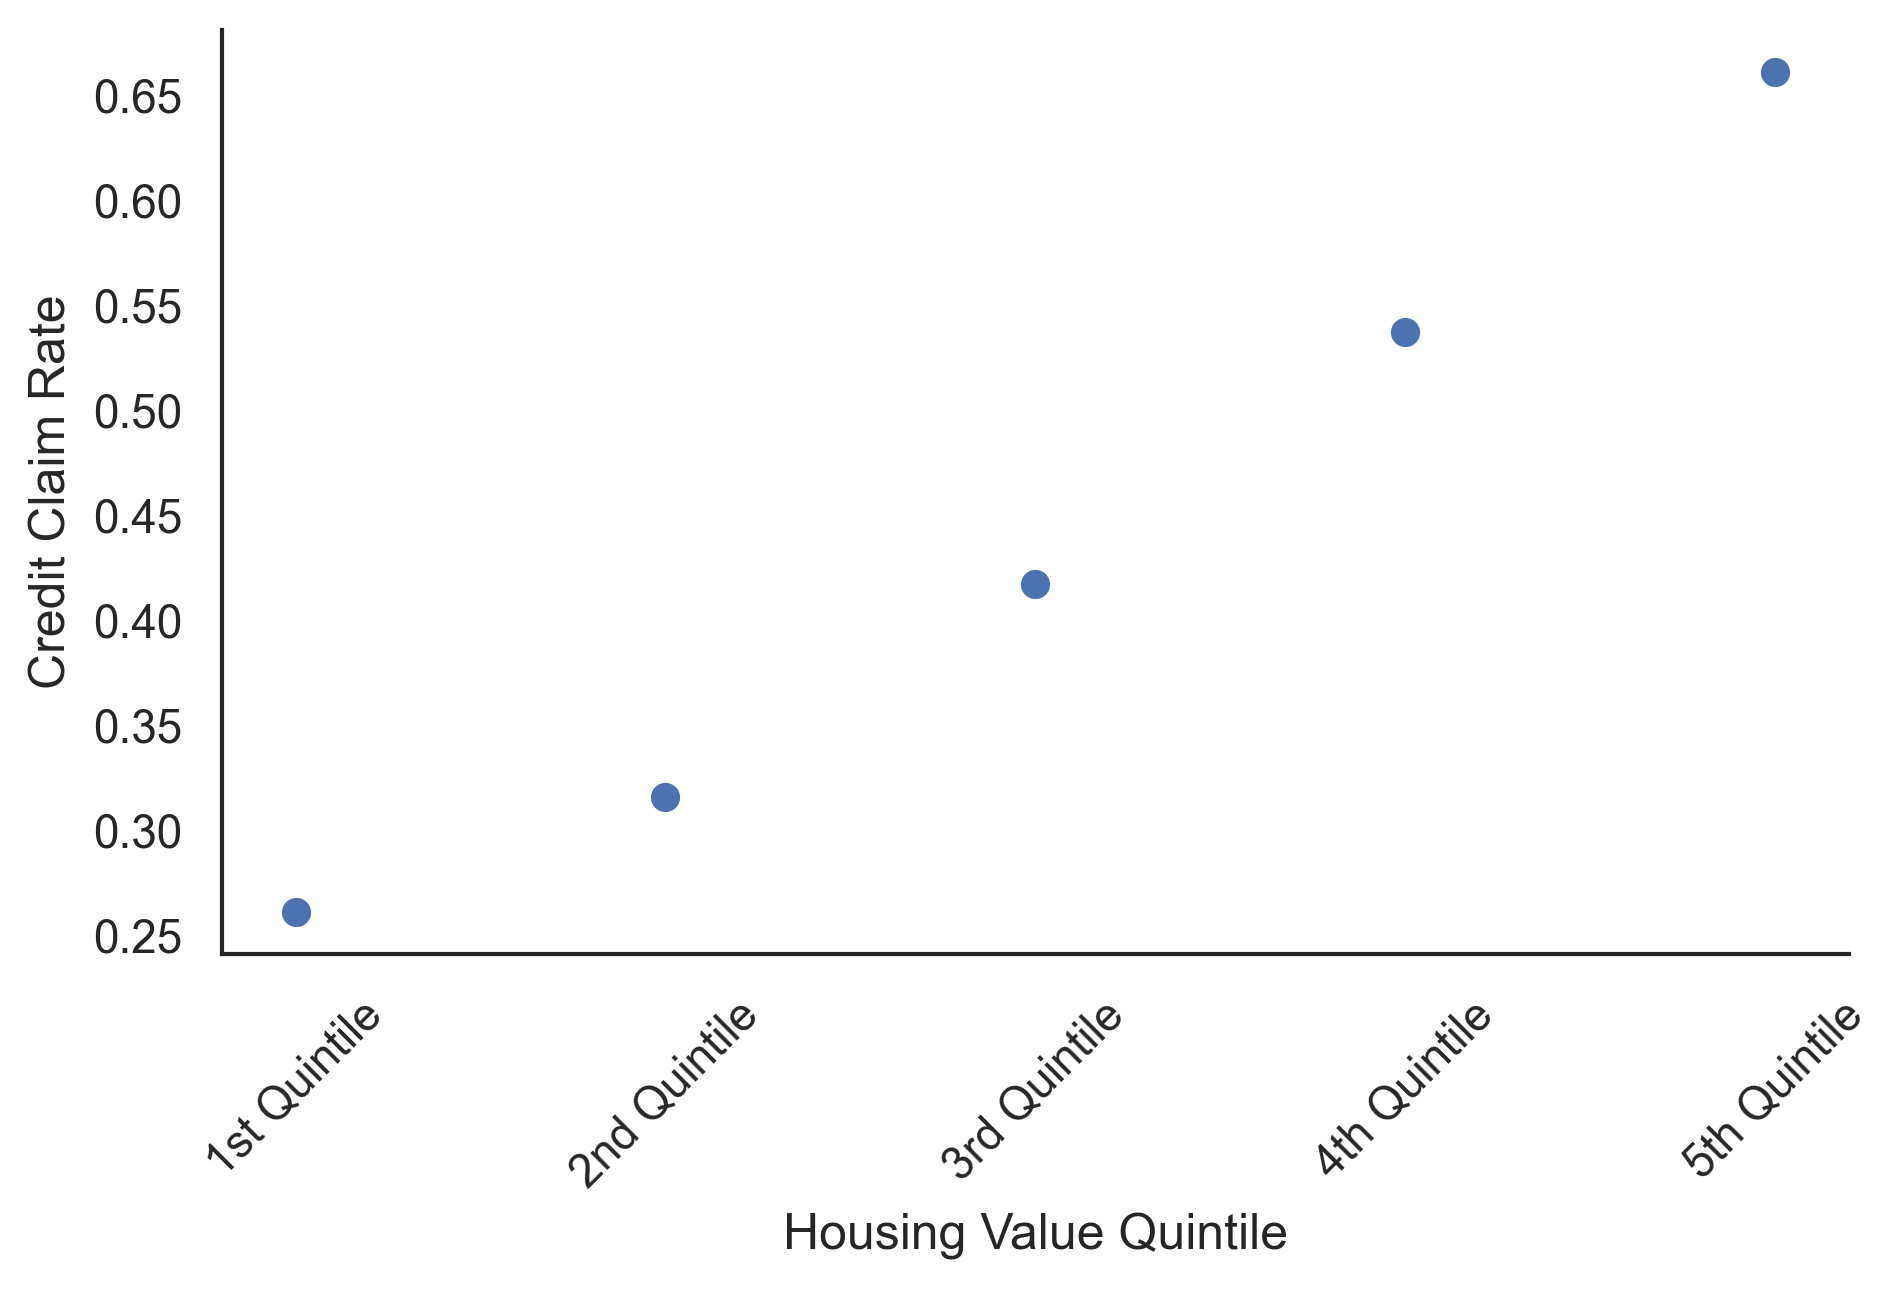
\includegraphics[width=0.8\textwidth]{figures/credit_by_zestimate_quintile.png}
    \caption{Credit claim rate by housing value quintile}
    \label{fig:credit_by_zestimate_quintile}
    %   \begin{flushleft}
    %     \footnotesize Note: The rate is c
    % \end{flushleft}
\end{figure}

We estimate model (5) of the main regression for the two tax credit program periods (SMDTC and NSMDTC) separately to examine whether some of the distributional effects change over time. \autoref{tab:reg_by_program} reports the regression results. \autoref{fig:coefficient_trend} shows the time trend of the household-level explanatory variable coefficients.

\begin{table}[!ht] \centering
  \caption{Regression results on state credit claim by program period}
  \label{tab:reg_by_program}
  \resizebox{0.9\textwidth}{!}{
\begin{tabular}{@{\extracolsep{5pt}}lcc}
\\[-1.8ex]\hline
\hline \\[-1.8ex]
& \multicolumn{2}{c}{\textit{Dependent variable: State Credit}} \
\cr \cline{2-3}
\\[-1.8ex] & \multicolumn{1}{c}{First round, SMDTC} & \multicolumn{1}{c}{Second round, NSMDTC}  \\
  & (before 2016) & (after 2020) \\
\hline \\[-1.8ex]
 System capacity & 0.002$^{}$ & 0.010$^{***}$ \\
& (0.002) & (0.002) \\
 Log Zestimate & 0.024$^{}$ & 0.251$^{***}$ \\
& (0.021) & (0.020) \\
 Year built & -0.001$^{**}$ & -0.001$^{***}$ \\
& (0.000) & (0.000) \\
 Log Housing size (sq ft) & 0.033$^{}$ & -0.062$^{**}$ \\
& (0.021) & (0.020) \\
 \# of Bedrooms & 0.004$^{}$ & -0.016$^{**}$ \\
& (0.007) & (0.006) \\
 \% population with bachelor degree ($>$25) & 0.207$^{**}$ & 0.170$^{***}$ \\
& (0.065) & (0.045) \\
 Owner occupancy rate & 0.091$^{**}$ & 0.026$^{}$ \\
& (0.033) & (0.048) \\
 Mortgage rate & -0.300$^{***}$ & -0.095$^{}$ \\
& (0.047) & (0.051) \\
 Log Area Median Income & 0.026$^{}$ & -0.008$^{}$ \\
& (0.023) & (0.019) \\
 Log Population & 0.028$^{*}$ & 0.024$^{*}$ \\
& (0.012) & (0.010) \\
 Log Median Age & 0.182$^{***}$ & -0.003$^{}$ \\
& (0.035) & (0.029) \\
 \% population identified as White & -0.252$^{***}$ & 0.007$^{}$ \\
& (0.069) & (0.051) \\
 \% population identified as Hispanic & -0.004$^{}$ & -0.152$^{***}$ \\
& (0.052) & (0.036) \\
 Urban share & 0.007$^{}$ & -0.033$^{*}$ \\
& (0.019) & (0.016) \\
 Within disadvantaged census tracts & -0.006$^{}$ & -0.038$^{***}$ \\
& (0.016) & (0.011) \\
 Year Fixed Effects & Yes & Yes \\
 County Fixed Effects & Yes & Yes \\
\hline \\[-1.8ex]
 Observations & 8326 & 16908 \\
 $R^2$ & 0.382 & 0.112 \\
 Adjusted $R^2$ & 0.380 & 0.111 \\
 Residual Std. Error & 0.386 & 0.453 \\
 F Statistic & 160.188$^{***}$ & 71.071$^{***}$ \\
\hline
\hline \\[-1.8ex]
\textit{Note:} & \multicolumn{2}{r}{$^{*}$p$<$0.05; $^{**}$p$<$0.01; $^{***}$p$<$0.001} \\
\end{tabular}}
\end{table}

In the first program period (before 2016), around 60\% of the systems claimed tax credits, whereas in the second period (after 2020), the rate dropped to 36\%. Under SMDTC, none of the housing characteristics significantly impacted the probability of claims. However, census tract characteristics such as higher educational levels, higher owner occupancy rates, higher median age, and lower percentage of white population increased the probability of credit claims. In contrast, under NSMDTC, housing value has a significantly positive impact on the outcome. Moreover, census tracts with higher Hispanic populations and those that are disadvantaged have fewer claims.

The change in determining characteristics for credit claims over time suggests discernible differences between early and late adopters of solar PV. Early adopters are likely to be more tech-savvy and have a preference for clean energy. For them, the likelihood of claiming the credit depends on their awareness of the program, which is potentially correlated with education level, and their financial savviness, potentially correlated with age and racial status. Additionally, if the system is under a leasing contract, potentially correlated with the mortgage rate, it is less likely to receive credit. Late adopters, on the other hand, could be more motivated by the financial gains of installing solar. Therefore, they are more sensitive to the financial benefits of the tax credit, as shown by the significant positive effect of system capacity in the second period.

The findings also reveal persistent equity issues, as disadvantaged and Hispanic-majority census tracts are less likely to benefit from tax credits under the NSMDTC. A notable difference between SMDTC and NSMDTC is the introduction of an aggregate cap under NSMDTC. This cap negatively affects distributional equity by imposing a negative effect on areas that are disadvantaged and have higher Hispanic populations. Thus, these results support increasing the aggregate cap and allowing for retroactive tax credit applications from rejected applications due to the cap being reached between 2021 and 2023, as passed by the new House Bill 252 \parencite{newsolarcap}. 

\subsection{The intensive margin of tax credit claim}

To deepen our understanding of the determinants of tax credit claims, we explore the intensive margin—that is, conditional upon receiving tax credits, which household characteristics lead to higher claimed amounts? To address this question, we employ the following OLS regression with the claimed amount as the dependent variable:

\begin{equation}\label{reg_4}
    \log(\text{TaxCreditAmount})_{ht} = \alpha + \beta X_{ht} + \gamma C_{lt}  + \delta_t + \varepsilon_{lt},
\end{equation}
where TaxCreditAmount$_{ht}$ is the dollar amount tax credit approved for household $h$ in year $t$, $X_{ht}$ is a vector of household level explanatory variables, $C_{lt}$ is a vector of census tract demographic controls, $\delta_t$ is the year fixed effect, and $\varepsilon_{lt}$ is the error term clustered at the census tract level. $\beta$ is the vector of coefficients of interest. We test three model specifications: (1) with only household-level variables, (2) adding census tract controls, and (3) incorporating year-fixed effects. \autoref{tab:sum_stat_dis_intensive} provides the summary statistics, and \autoref{tab:reg_claim_amount} displays the regression results.

\begin{table}[!ht] \centering 
  \caption{Regression results of linear models for tax credit claim amount} 
  \label{tab:reg_claim_amount} 
 \resizebox{0.6\textwidth}{!}{
 \begin{tabular}{@{\extracolsep{5pt}}lccc} 
\\[-1.8ex]\hline 
\hline \\[-1.8ex] 
 & \multicolumn{3}{c}{\textit{Dependent variable:}} \\ 
\cline{2-4} 
\\[-1.8ex] & \multicolumn{3}{c}{Log(Tax credit amount)} \\ 
\\[-1.8ex] & (1) & (2) & (3)\\ 
\hline \\[-1.8ex] 
 System capacity & 0.109$^{***}$ & 0.112$^{***}$ & 0.115$^{***}$ \\ 
  & (0.001) & (0.001) & (0.002) \\ 
  Log Zestimate & 0.049$^{***}$ & 0.070$^{***}$ & 0.059$^{***}$ \\ 
  & (0.010) & (0.013) & (0.013) \\ 
  Year built & $-$0.001$^{***}$ & $-$0.001$^{***}$ & $-$0.001$^{***}$ \\ 
  & (0.0002) & (0.0002) & (0.0002) \\ 
  Log Housing size (sq ft) & 0.083$^{***}$ & 0.057$^{***}$ & 0.054$^{***}$ \\ 
  & (0.015) & (0.015) & (0.015) \\ 
  \# of Bedrooms & 0.026$^{***}$ & 0.027$^{***}$ & 0.028$^{***}$ \\ 
  & (0.005) & (0.005) & (0.005) \\ 
 \hline \\[-1.8ex] 
Census Tract Controls & No & Yes & Yes \\ 
Year Fixed Effects & No & No & Yes \\ 
Observations & 11,034 & 11,034 & 11,034 \\ 
R$^{2}$ & 0.435 & 0.448 & 0.461 \\ 
Adjusted R$^{2}$ & 0.435 & 0.447 & 0.459 \\ 
\hline 
\hline \\[-1.8ex] 
\textit{Note:}  & \multicolumn{3}{r}{$^{*}$p$<$0.1; $^{**}$p$<$0.05; $^{***}$p$<$0.01} \\ 
\end{tabular}}
\end{table} 

The regression results highlight two primary factors influencing solar tax credit claims. First, higher system capacity consistently leads to higher tax credit claims across all model specifications. This trend is anticipated, considering the tax credit amounts to 10\% of the total installation cost, and systems with greater capacity generally incur higher costs.

Secondly, households with higher property values claim larger tax credits. This observation raises concerns about equity within the subsidy program, as it suggests that wealthier households are reaping greater benefits from government solar incentives. This disparity could be perceived as exacerbating existing socioeconomic inequities by disproportionately favoring already affluent households. However, a deeper examination reveals that households with higher property values likely face higher costs for installing solar systems of the same capacity. Factors contributing to these costs include the need for custom solutions to fit specific property aesthetics, the use of premium materials, more complex installation requirements, and stricter compliance with local regulations in affluent areas. 


We follow \textcite{borenstein_distributional_2016} to illustrate the concentration of solar credit claims by income quintile and calculate the concentration index for the full sample period, SMDTC, and NSMDTC. \autoref{fig:credit_claim_distribution} shows the concentration curves for the three samples. The 45-degree line represents perfect equality; the more convex the curve, the more regressive the policy, favoring wealthier households. The curves indicate that NSMDTC is less equitable than SMDTC. The concentration index, calculated as the ratio of the area between the concentration curve and the 45-degree line over the total area under the 45-degree line, for the full sample, SMDTC, and NSMDTC are 0.444, 0.498, and 0.405, respectively.\footnote{If we use the full credit claim data from EMNRD for the study period, the concentration index for the full sample, SMDTC, and NSMDTC are 0.387, 0.449, and 0.356, respectively. This suggests that solar adopters are shifting towards low-income populations as the market matures, and the distributional inequality gap is shrinking. \autoref{fig:concentration_index} shows the year trend of the concentration index.}%This comparison underscores the need for continuous evaluation and adaptation of incentive programs to address the lack of credit claims among less wealthy solar adopters, likely due to systems being leased rather than owned.
\textcite{borenstein_distributional_2016} showed that the concentration index for the federal Residential Energy Credit, which is the federal solar tax credit, is 0.606, higher than what we find at the state level. %We want to note the differences between our two approaches. \textcite{borenstein_distributional_2016} used individual tax return data from the Internal Revenue Service, and the concentration data is calculated based on the percentage claimed in each income bracket of all tax filers. Since we do not observe individual income levels and solar tax credit claims in the same dataset, we made the following adjustments to their approach. First, we calculate the concentration index conditional on solar adoption and credit claims. As we show in \autoref{sec:adoption_equity}, lower-income households are less likely to adopt solar, so our sample already has an upward bias on the income bracket. Second, we do not observe household income level and therefore used estimated housing value (Zestimate) as a proxy for household wealth. Although income and wealth are positively correlated, this approach may still capture other aspects of household differences that are not income-related. These two methodological differences may result in a much lower concentration index compared to similar policies.

\begin{figure}[!ht]
    \centering
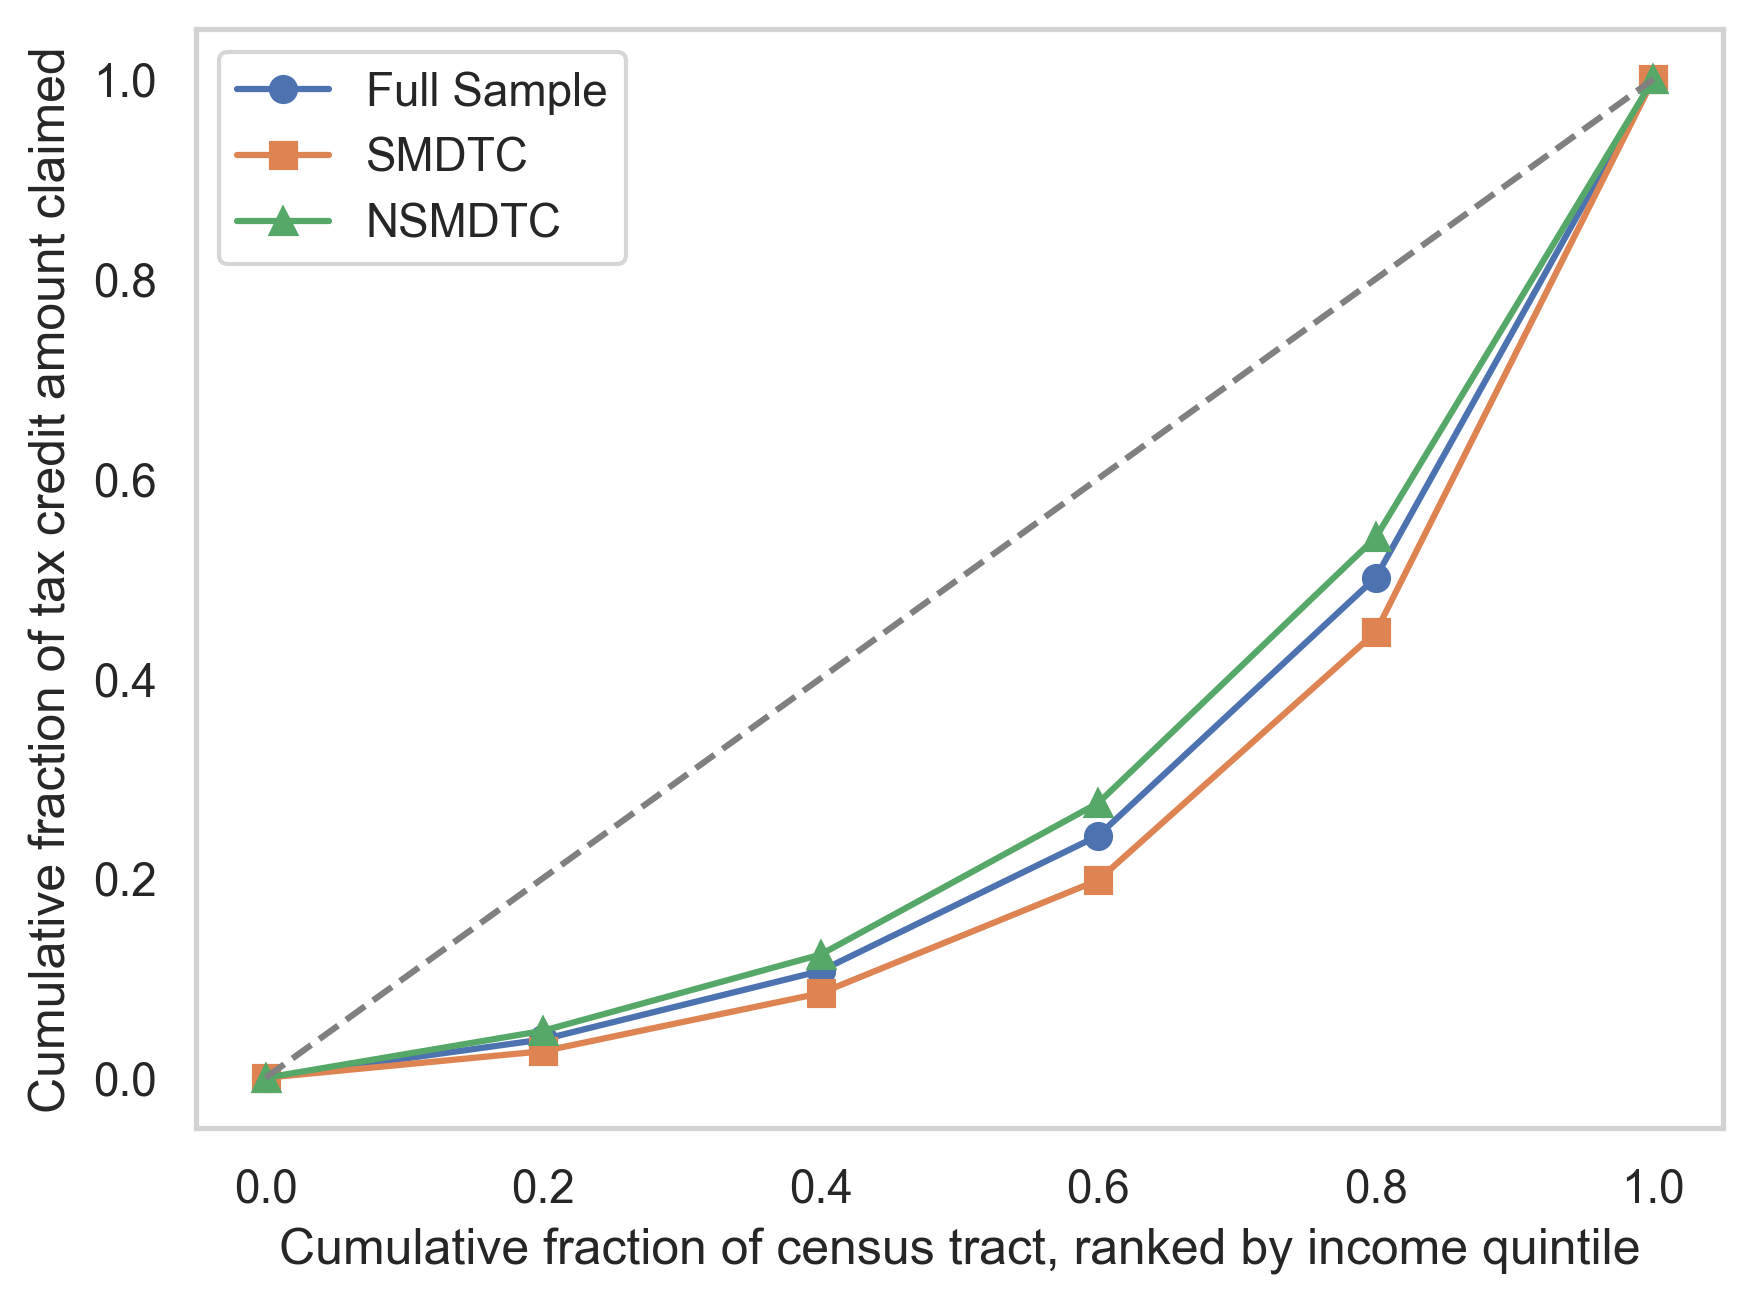
\includegraphics[width=0.8\textwidth]{figures/credit_claim_amount_distribution_by_income.png}
    \caption{Concentration curves of solar tax credit}
    \label{fig:credit_claim_distribution}
    \begin{flushleft}
        \footnotesize Note: The 45-degree line indicates perfect equality. The concentration index can be calculated as the ratio of the area between the concentration curve and the 45-degree line over the total area under the 45-degree line. The index would take values between -1 and 1. An index value of zero indicates perfect equality. 
    \end{flushleft}
\end{figure}


These insights indicate that while the tax credit scheme is effective in promoting solar adoption, it tends to favor wealthier households. This observation calls for reviewing policy designs to ensure that solar energy benefits are more equitably distributed, thereby supporting broader access to renewable energy across different socioeconomic groups. Further research is also warranted to explore the reasons behind price variations in solar system installations across different households.


%%%%%%%%%%%%%%%%%%%%%%%%%%%%%%%%%%%
\section[Conclusion]{Conclusion and policy implications}

This research aims to understand the landscape of residential solar PV adoption in New Mexico through the lenses of two aspects of equity: adoption equity and distributional equity. For adoption equity, we examine whether the rate of adoption is equitable across census tracts with varying racial, ethnic, income, and education compositions, both at the extensive and intensive margins. For distributional equity, we focus on whether the state solar tax credit is equitably distributed across solar households.

In terms of adoption equity, we find little disparity between racial and ethnic groups, contrary to findings from other research on solar equity in other parts of the U.S. Moreover, the existence of the state solar tax credit diminishes any remaining disparities across racial and ethnic groups. However, significant income disparity remains at both the extensive and intensive margins. Census tracts that are overburdened on other socioeconomic aspects are also correlated with lower solar adoption. Although the solar tax credit reduces some of these disparities, it is not sufficient to alleviate them fully. Education disparity only exists among early adopters and higher-income areas and has relatively small effects on solar adoption rates.

Conditional on solar adoption, the results reveal significant disparities in the distribution of solar tax credits in New Mexico. Credit claims are concentrated among households adopting large solar capacities and with higher housing values. Communities with higher education levels, higher owner-occupied housing rates, lower mortgage rates, and lower Hispanic population shares also see higher rates of tax credit claims. The introduction of the aggregate cap under the NSMDTC has exacerbated these inequities, favoring wealthier households and negatively affecting disadvantaged and Hispanic-majority census tracts.

We conclude with the following remarks. First, although the findings highlight persistent equity issues, especially stemming from income disparity and disadvantaged status, this inequality is smaller compared to what the literature has found. The diverse racial and ethnic composition in New Mexico may have contributed to greater solar adoption equity compared to other states.

Second, we show that disadvantaged and Hispanic-majority census tracts are less likely to benefit from tax credits under the NSMDTC, potentially due to the information barrier of the application process and the aggregate cap being imposed. However, we acknowledge that the NSMDTC has undergone some recent changes, including raising the aggregate cap and allowing for retroactive credit claims for rejected applications from 2021 to 2023 due to the cap being met \parencite{newsolarcap}, and changing the tax credit from nonrefundable to refundable \parencite{nmsmdtc}. These policy changes will likely relieve some of the distributional issues. Yet, since leased systems do not qualify for tax credits, and lower-income households are more likely to lease systems rather than own them, we will still see a concentration of credit claims among wealthier households. Additionally, there is a need for targeted outreach and support to disadvantaged communities to ensure they are aware of and can overcome the information barriers to these incentives.

To enhance the equity of solar tax credits and other incentives, we recommend the continuous monitoring of existing policy impacts and adjusting it based on adoption rates and feedback from underserved communities. Introducing specific incentives or additional support for low-income households and those in disadvantaged areas can help reduce the financial and informational barriers to solar adoption. Implementing educational campaigns and providing resources to ensure that all communities are aware of available incentives and how to access them are also essential steps. 

Future research should explore the long-term impacts of recent policy changes on the equity of solar adoption, the effectiveness of targeted outreach programs in increasing solar adoption in disadvantaged communities, and comparative studies across different states to identify best practices in promoting equitable solar adoption. Additionally, estimating the effect of community solar programs on equity, particularly how these programs can enhance access to solar energy for households that cannot afford individual installations or do not own their homes, is a vital area for future research.


While this study provides valuable insights, it is limited by the availability of data on individual household characteristics. Future studies with more granular data could provide a deeper understanding of the equity issues in solar adoption. By addressing these aspects, policymakers can better design and implement solar incentive programs that promote equitable access and adoption across all socioeconomic groups, ensuring a just and inclusive energy transition in New Mexico.



%%%%%%%%%%%%%%%%%%%%%%%%%%%%%%%%%%%
\newpage
\appendix
\numberwithin{equation}{section}
\numberwithin{figure}{section}
\numberwithin{table}{section}
\section[Appendix]{Appendix}

\subsection{Variable calculation methods}
\label{subsec:Variable_Cal}
\subsubsection*{Census tract mapping}
To map 2020 Decennial Census-level data into 2010 Decennial, we refer to the 2020 Census Redistricting Data (P.L. 94-171) Block Relationship files \footnote{\url{https://www.census.gov/geographies/reference-files/time-series/geo/relationship-files.2020.html}}. We use the land area of the overlapping part (in square meters) divided by the total land area of 2010 tract to calculate the share of 2020 tract land overlapping into each 2010 tract, and then build a $612 \times 499$ matrix. Then, we convert each census tract-level variable into a $612 \times 1$ matrix, and multiply with the mapping matrix to get the $499 \times 1$ data matrix.

\subsubsection*{Built year group}
We define the house built year group as follows: Built after 2020 = 1; Built between 2010 and 2019 = 2; Built between 2000 and 2009 = 3; Built between 1990 and 1999 = 4; Built between 1980 and 1989 = 5; Built between 1970 and 1979 = 6; Built between 1960 and 1969 = 7; Built between 1950 and 1959 = 8; Built between 1940 and 1949 = 9. To determine the built year group of the median house in each census tract-year, we use the total number of housing units provided by the U.S. Census Bureau DP04 table. We identify the built year group  of the median housing unit by ranking the built year groups from earliest to latest. The built year group of the median unit is then assigned to the entire tract-year.

\subsubsection*{Racial diversity}
The racial diversity is defined as:
\begin{equation}
\text{Racial diversity} = \sum_{i} (\frac{\text{Population identified as race }i}{\text{Total one-race population}})^2
\end{equation}
where $i = $ White, Black or African American, American Indian and Alaska Native,	Asian, Native Hawaiian and Other Pacific Islander, and other race.

\subsubsection*{Electricity price}
We determine the electricity provider for each census tract and the company's ownership each year using data from the Homeland Infrastructure Foundation Level Data (HIFLD). Additionally, we obtain the electricity price for each company annually from the Energy Information Administration's Table 6 (T6). We then calculate the tract-year electricity price as the average electricity price of all providers in each tract for each year.


\subsubsection*{Credit}
We generate $Credit$ for each year to show the state solar incentive availability as follows.  
\[
\text{Credit} = 
\begin{cases} 
 0 & \text{if } \text{Year} = 2017, 2018, 2019 \\
 1 & \text{otherwise.}
\end{cases} 
\]


\subsection{Supplementary Figures}

\begin{figure}[H]
    \centering
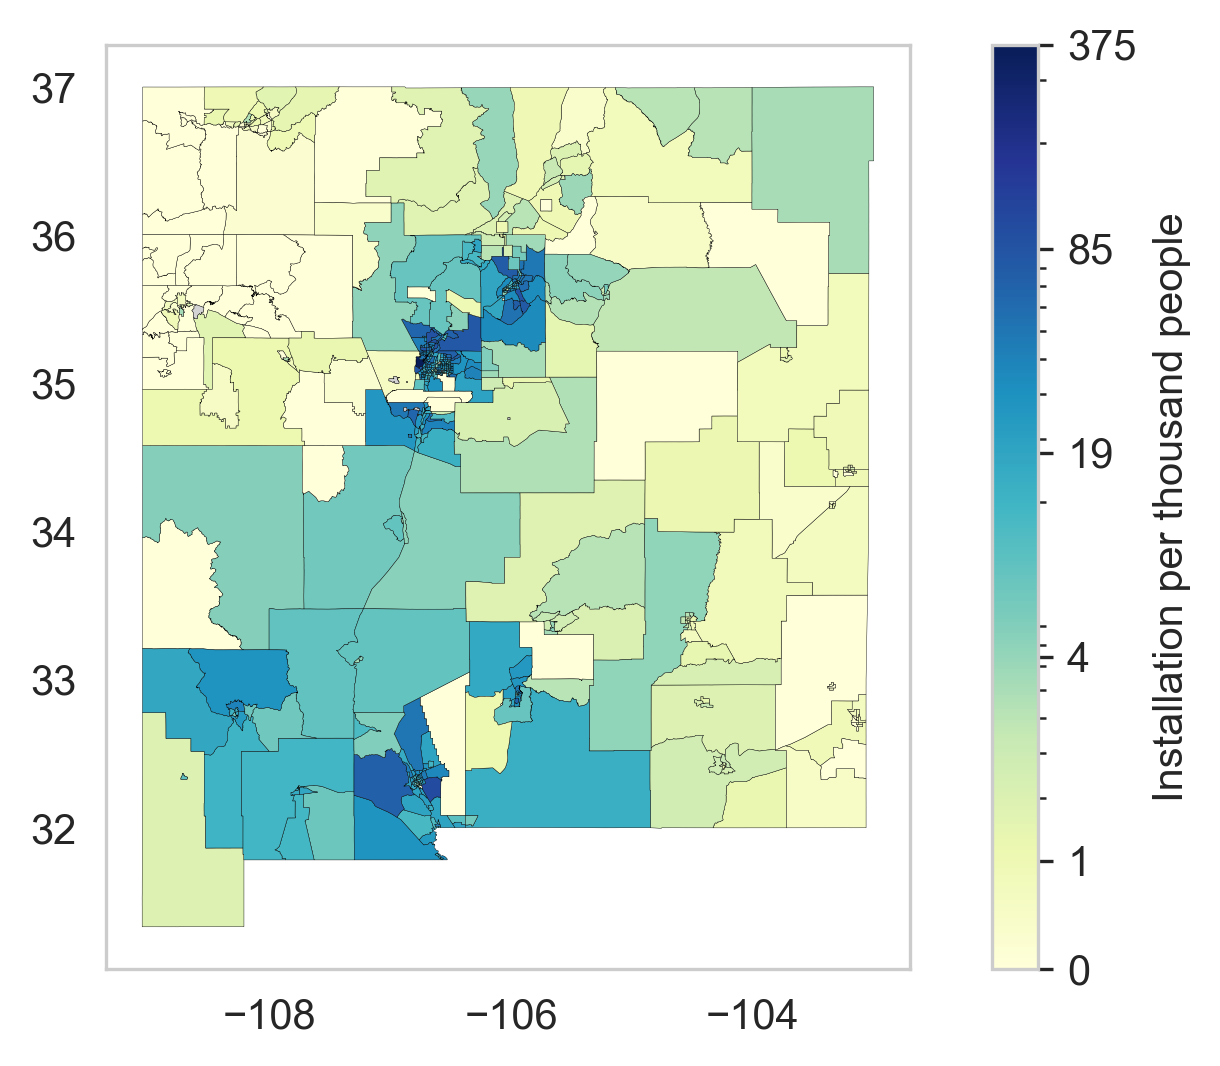
\includegraphics[width=0.7\textwidth]{figures/tract_count_per_kpop_map.png}
    \caption{Installation per thousand people by 2020 census tract}
    \label{fig:install_kpop}
      \begin{flushleft}
        \footnotesize Note: The total installation count is up to the end of 2023 for each census tract. The census tracts areas are defined in the 2020 Decennial Census. The tract-level population is taken at the 2022 level from the American Community Survey 1-year data. The legend is in logarithm scale. 
    \end{flushleft}
\end{figure}

\begin{figure}[H]
    \centering
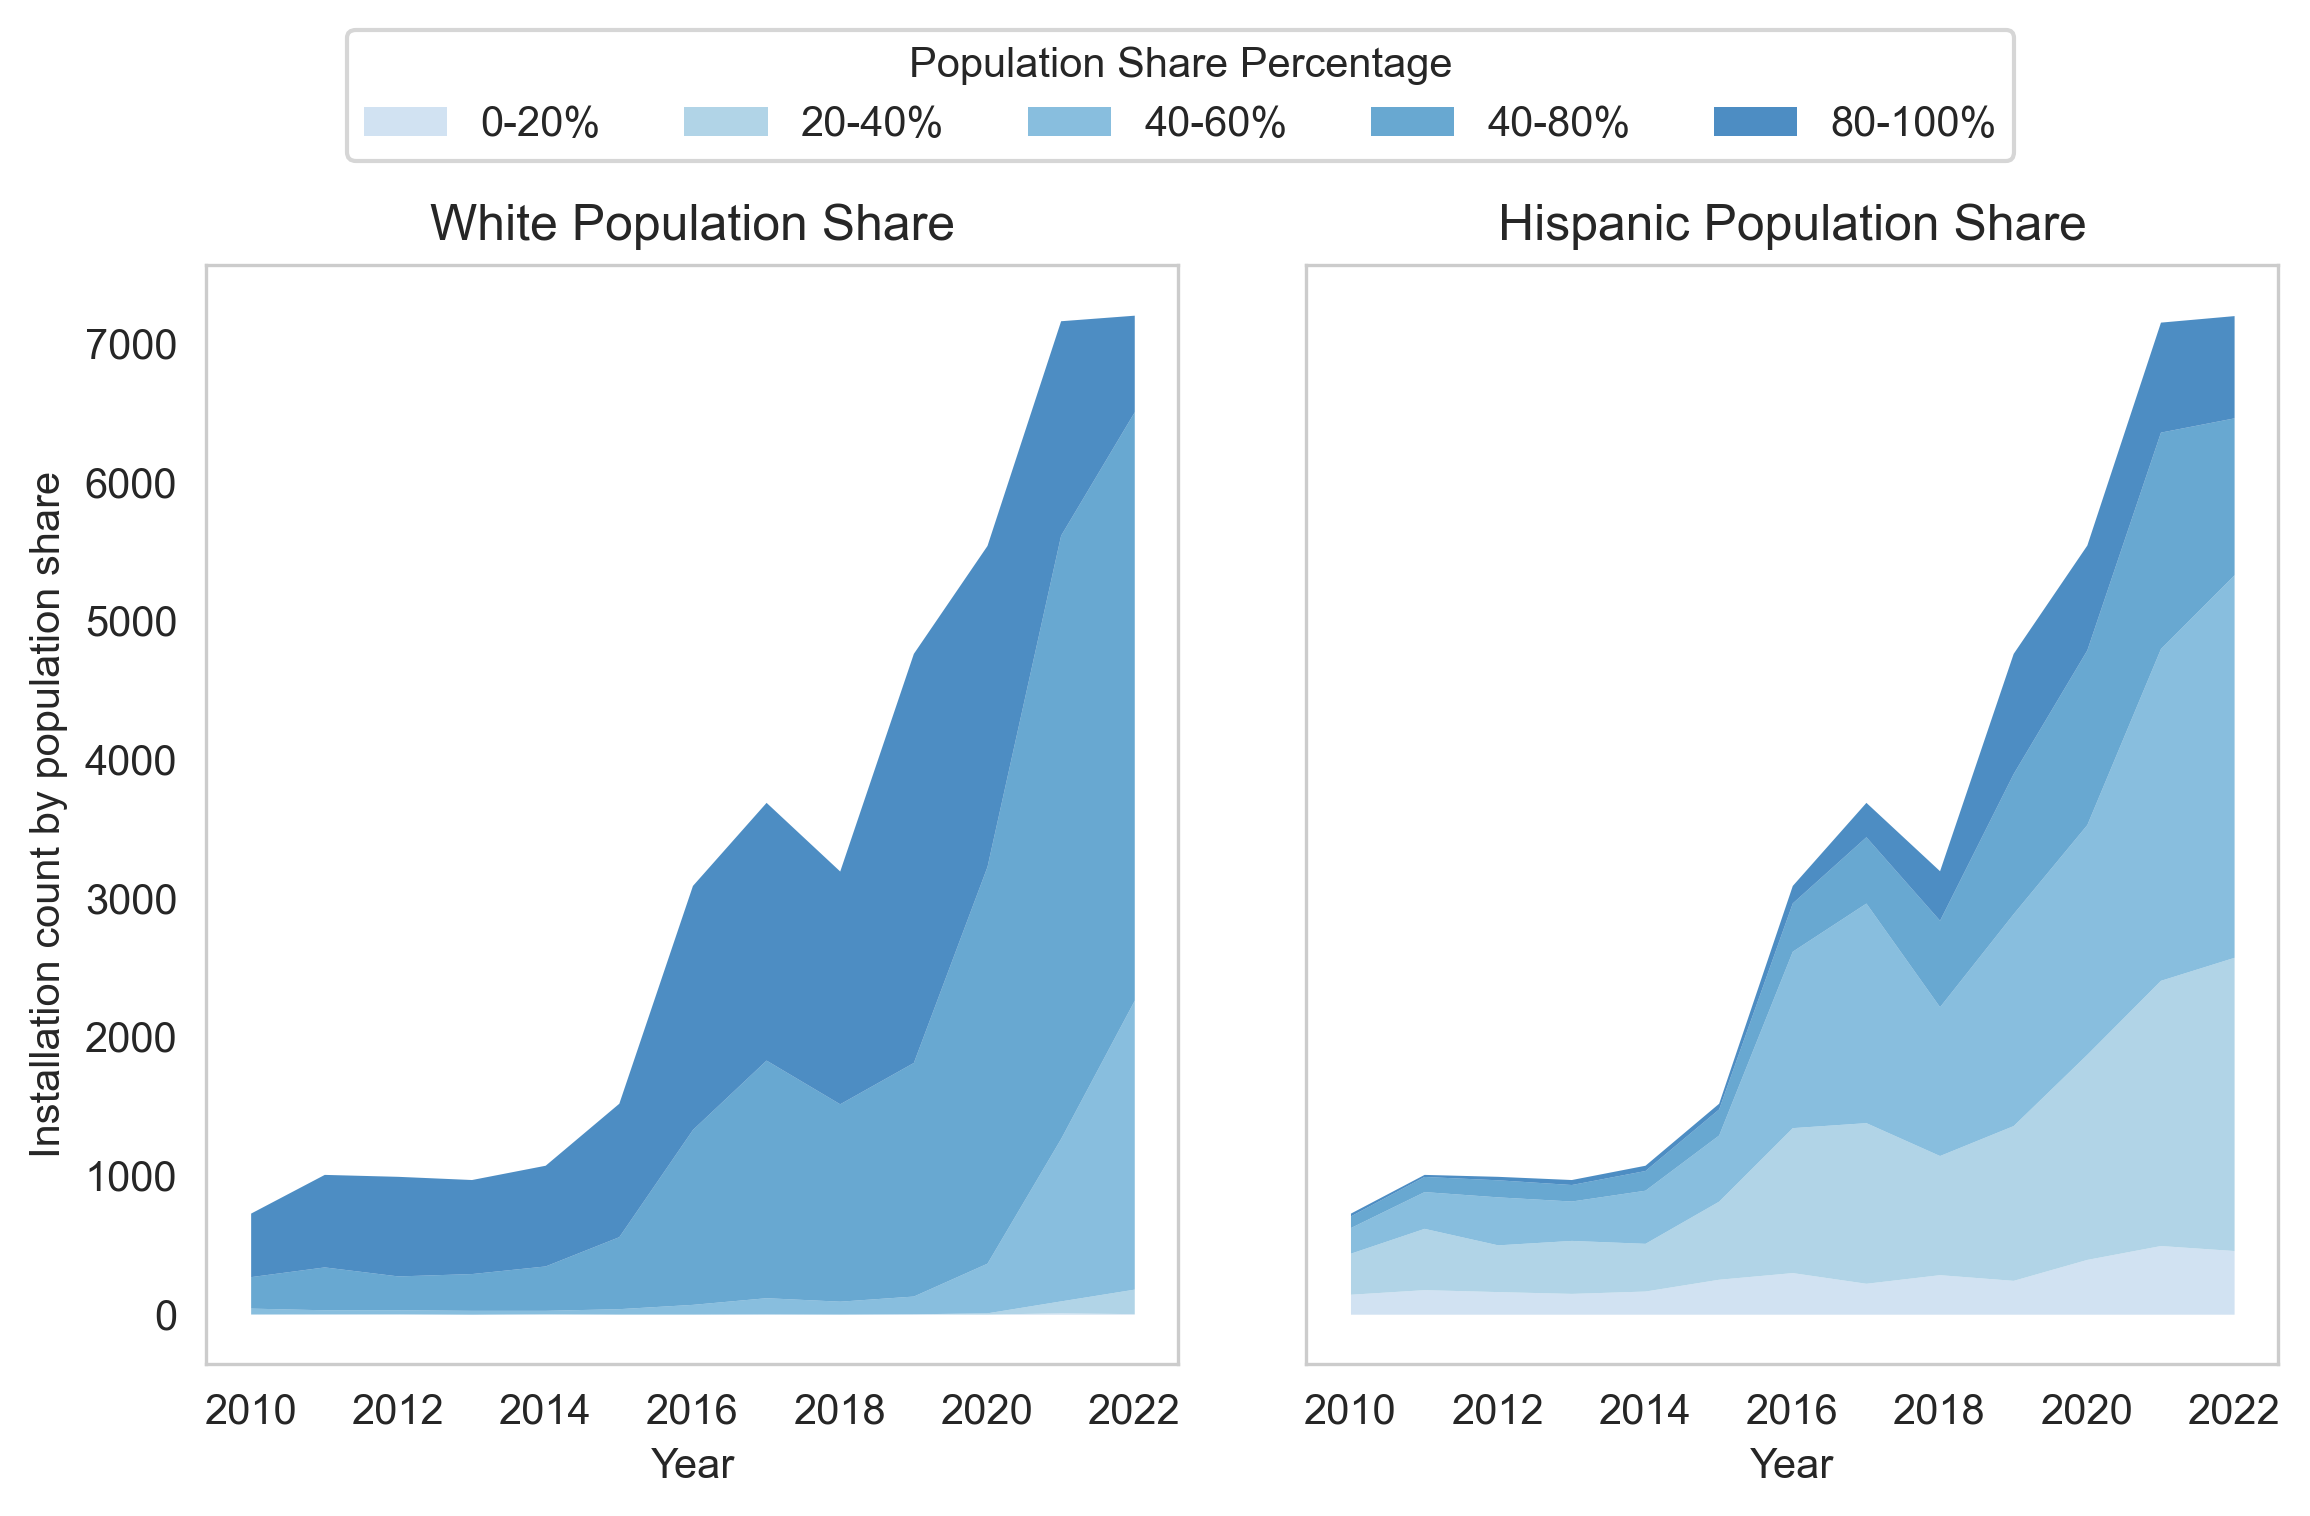
\includegraphics[width=1\textwidth]{figures/population_quintiles.png}
    \caption{Installation by racial population share}
    \label{fig:population_quintiles}
\end{figure}

\begin{figure}[H]
    \centering
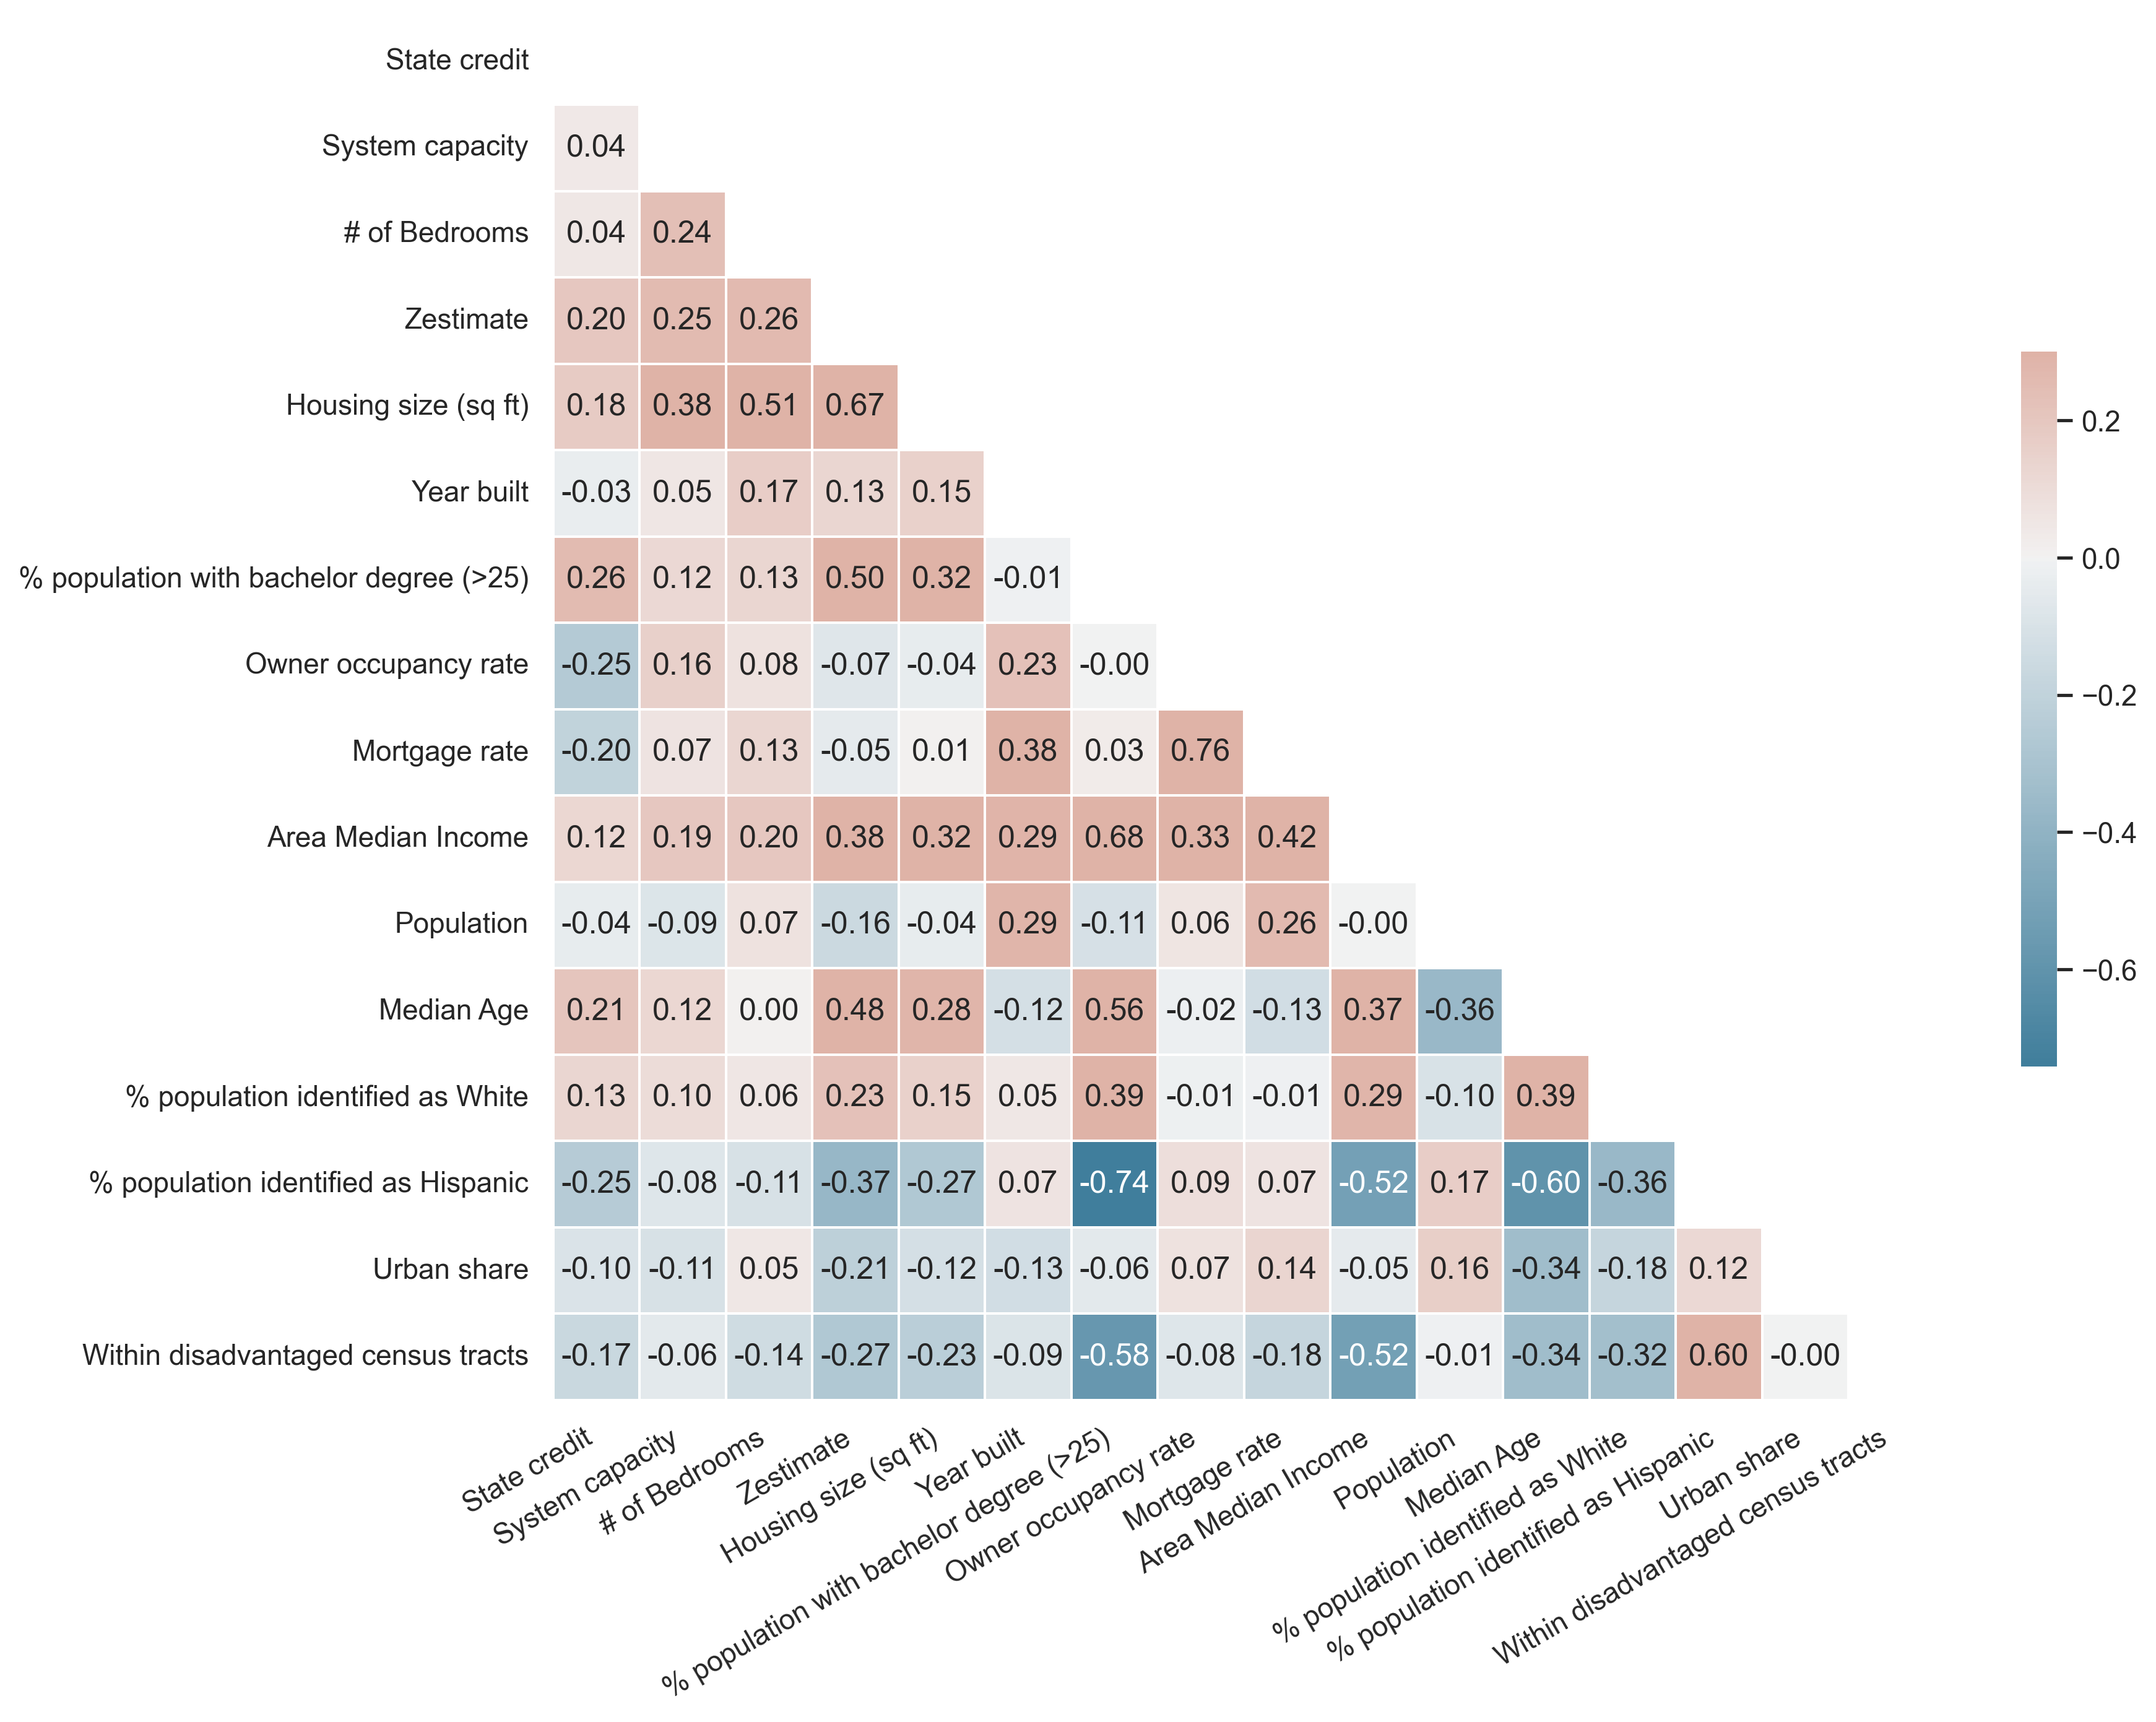
\includegraphics[width=1\textwidth]{figures/corr_matrix.png}
    \caption{Correlation matrix between regression variables in the distributional equity analysis}
    \label{fig:corr_matrix}
\end{figure}

\begin{figure}[H]
    \centering
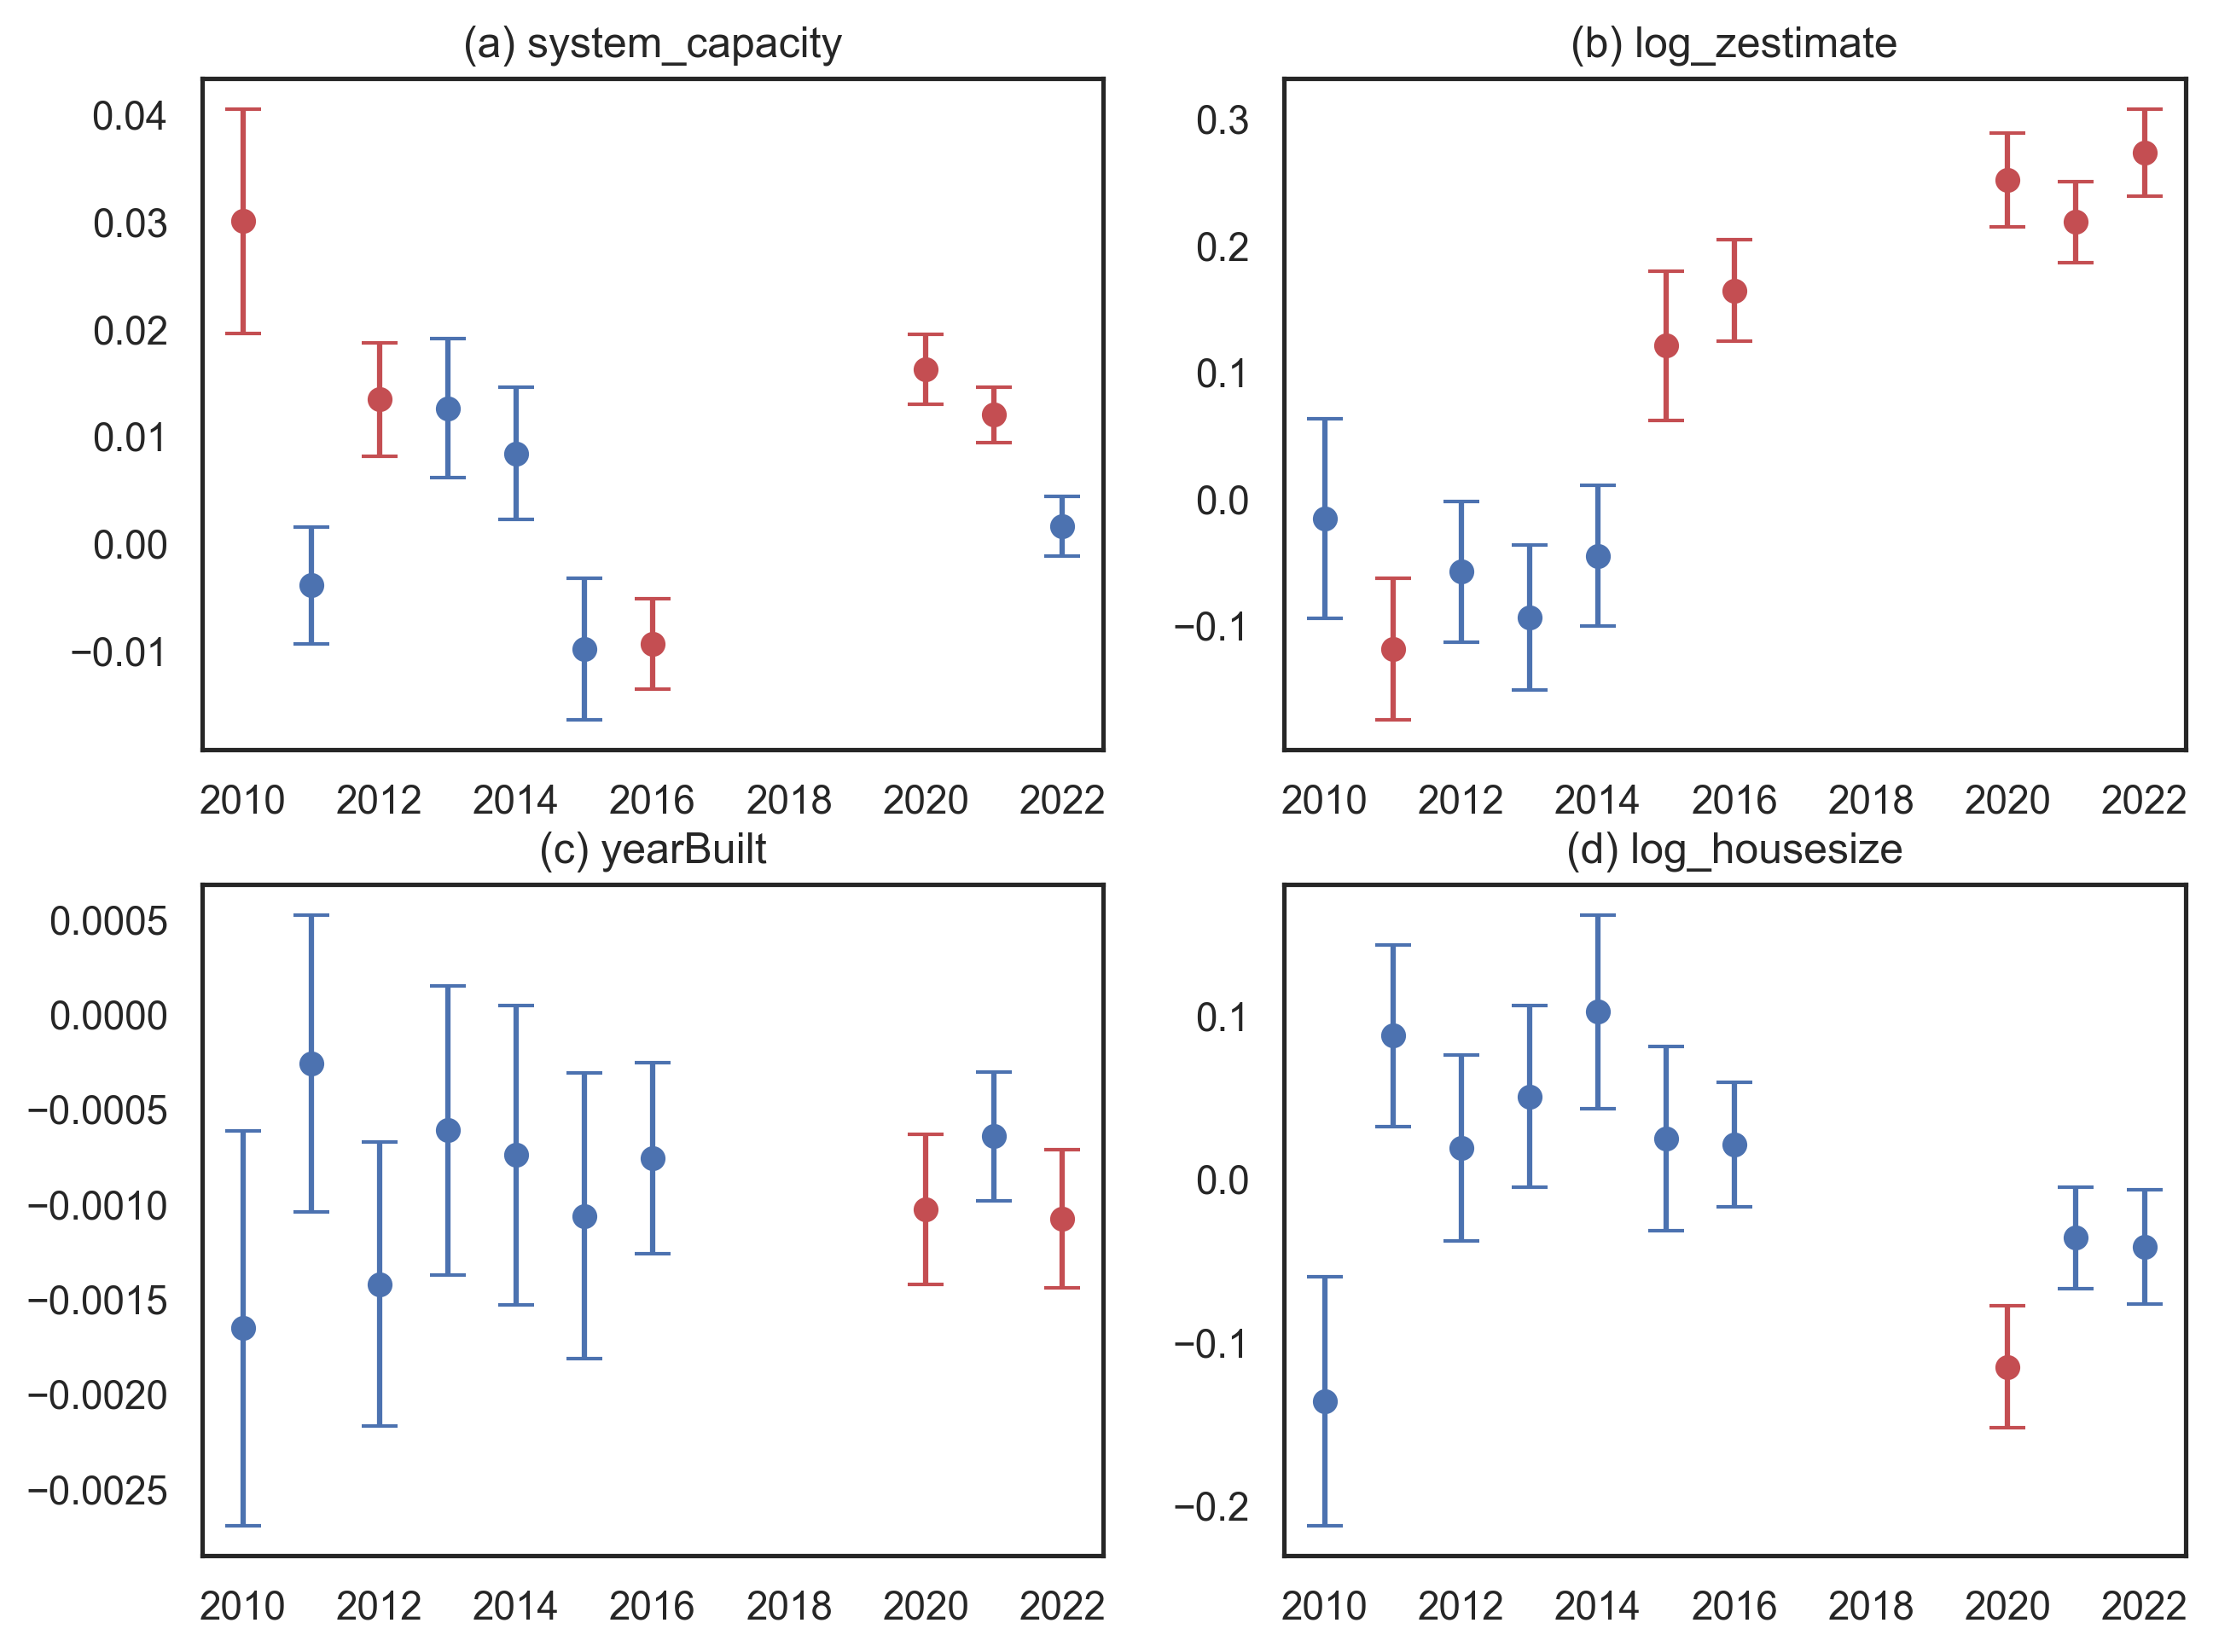
\includegraphics[width=1\textwidth]{figures/key_coefficient_trend.png}
    \caption{Coefficient trend by year for household-level explanatory variables}
    \label{fig:coefficient_trend}
\end{figure}

\begin{figure}[H]
    \centering
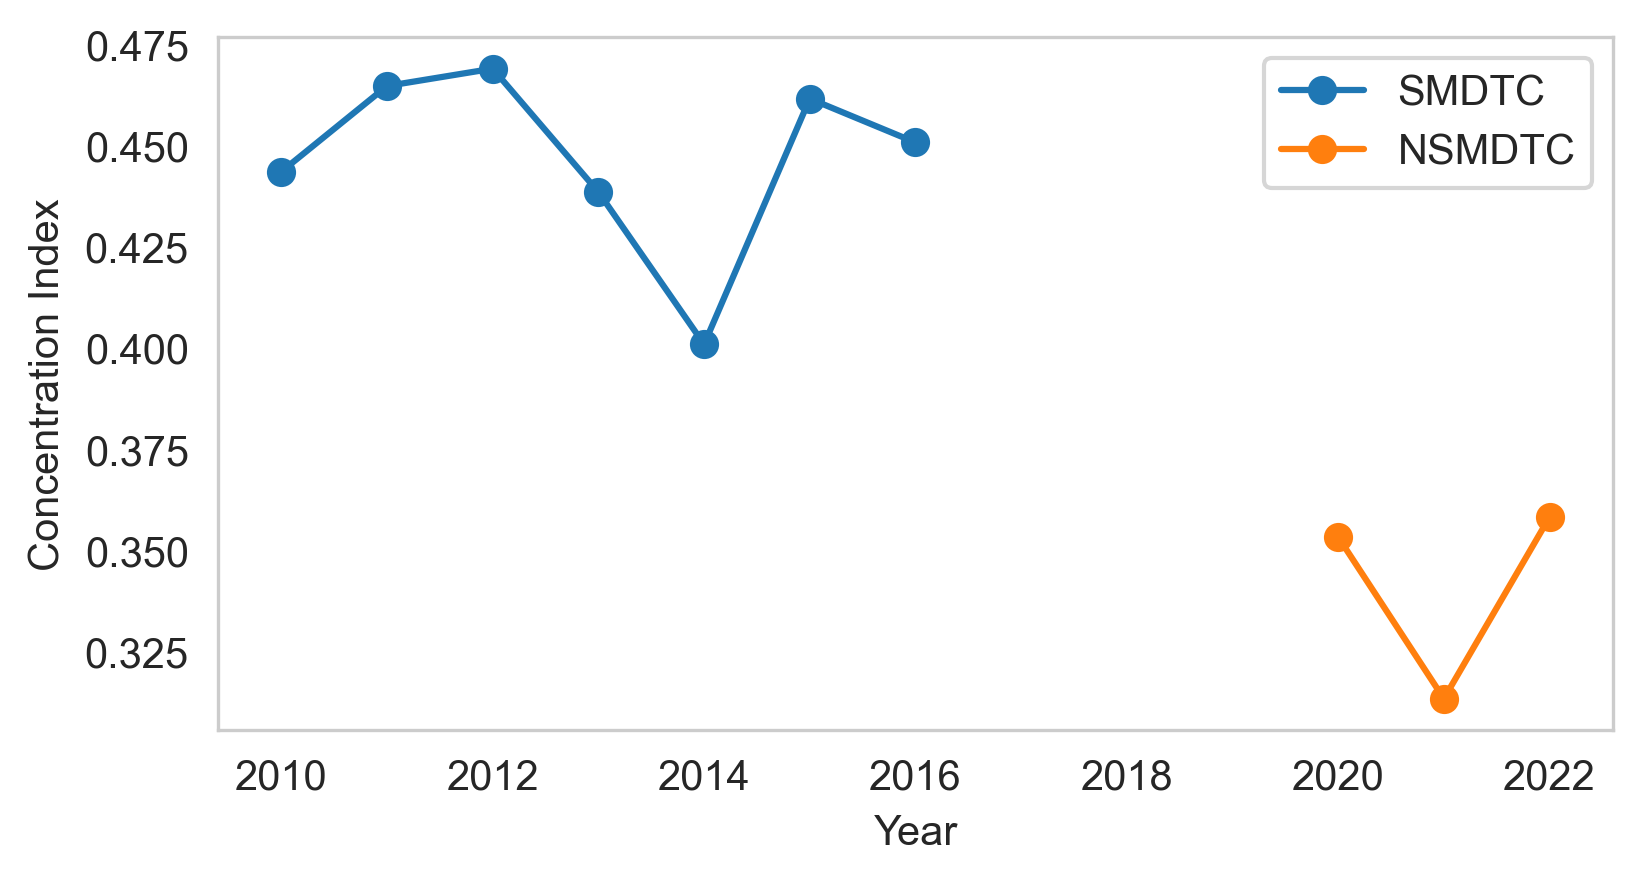
\includegraphics[width=0.9\textwidth]{figures/concentration_index_by_year.png}
    \caption{Concentration index of state tax credit distribution by year}
    \label{fig:concentration_index}
          \begin{flushleft}
        \footnotesize Note: The concentration indices are calculated using the EMNRD credit claim data from 2010 to 2022.  
    \end{flushleft}
\end{figure}

\newpage

\subsection{Supplementary Tables}

\begin{table}[H]
\centering
\singlespacing
\caption{Summary statistics of regression model (\ref{reg_1}) }
\label{tab:first-stage summary stat}
\resizebox{0.9\textwidth}{!}{%
\begin{tabular}{lrrrrrr}
\hline
\multicolumn{1}{r}{} & N & Mean & Std. Dev. & Median & Max & Min \\ \hline
% Count & 6474 & 6.33 & 12.58 & 1 & 155 & 0 \\
Having installation & 6474 & 0.59 & 0.49 & 1 & 1 & 0 \\
%Occ & 6474 & 84.67 & 12.26 & 88.38 & 100 & 0 \\
Owner occupied & 6474 & 45.33 & 22.72 & 47.27 & 100 & 0 \\
%HHSize & 6474 & 2.68 & 0.75 & 2.59 & 21.38 & 0 \\
Electricity & 6474 & 17.64 & 14.86 & 12.21 & 100 & 0 \\
%MTG & 6474 & 28.06 & 14.51 & 26.36 & 81.12 & 0 \\
Built year group & 6474 & 5.18 & 1.45 & 5 & 10 & 1 \\
Utility type & 6474 & 2.72 & 1.71 & 2 & 6 & 1 \\
PNM & 6474 & 0.41 & 0.49 & 0 & 1 & 0 \\
Electricity price & 6474 & 13.01 & 1.83 & 13.08 & 21.11 & 7.78 \\
Installation price & 6474 & 5.68 & 1.33 & 5.30 & 9 & 4.30 \\
Temperature & 6474 & 14.03 & 2.83 & 14.40 & 18.90 & 3.68 \\
GHI & 6474 & 2034.01 & 59.10 & 2035.95 & 2189.54 & 1816.68 \\
%HSGrad & 6474 & 26.76 & 8.8 & 27.04 & 57.3 & 0 \\
Bachelor & 6474 & 25.92 & 16.48 & 21.95 & 81.78 & 0 \\
%HV & 6474 & 159112.05 & 114572.15 & 143100 & 851600 & 0 \\
Income & 6474 & 49333.93 & 21219.96 & 45054 & 174019.73 & 7278.34 \\
Population & 6474 & 4022.10 & 1805.60 & 3819 & 17497 & 71.02 \\
%Male & 6474 & 49.57 & 4.41 & 49.39 & 100 & 27.57 \\
Racial diversity & 6474 & 0.65 & 0.16 & 0.66 & 1 & 0.22 \\
White & 6474 & 72.31 & 21.71 & 78.43 & 100 & 0.16 \\
Non-Hispanic White & 6474 & 39.99 & 21.77 & 40.54 & 95.78 & 0 \\
Hispanic & 6474 & 45.82 & 23.42 & 44.31 & 100 & 0 \\
Total housing unit & 6474 & 1781.76 & 824.98 & 1680.50 & 8278 & 0 \\
Disadvantage & 6474 & 0.54 & 0.50 & 1 & 1 & 0 \\
Urban & 6474 & 73.28 & 38.64 & 98.08 & 100 & 0 \\
Credit & 6474 & 0.77 & 0.42 & 1 & 1 & 0 \\ \hline
\end{tabular}%
}
\end{table}


\begin{table}[H]
\centering
\singlespacing
\caption{Full results for regression model (\ref{reg_1})}
\label{tab:probability_regression_full}
\resizebox{0.8\textwidth}{!}{
\begin{tabular}{@{\extracolsep{2pt}}lcc}
\small
\\[-1.8ex]\hline
\hline \\[-1.8ex]
& \multicolumn{2}{c}{\textit{Dependent Variable: Having new installation}} \
\cr \cline{2-3}
\\[-1.8ex] & \multicolumn{1}{c}{Linear Probability} & \multicolumn{1}{c}{Logit Marginal Effect} \\
\hline \\[-1.8ex]
Hispanic & 0.001$^{**}$ & 0.001$^{***}$ \\
& (0.000) & (0.000) \\
White & 0.003$^{***}$ & 0.003$^{***}$ \\
& (0.000) & (0.000) \\
Log Area Median Income & 0.120$^{***}$ & 0.140$^{***}$ \\
& (0.019) & (0.018) \\
Bachelor & 0.003$^{***}$ & 0.004$^{***}$ \\
& (0.001) & (0.001) \\
Disadvantaged & 0.003 & 0.013 \\
& (0.013) & (0.012) \\
Log population & 0.022 & 0.0433* \\
 & (0.023) & (0.022) \\
Electricity & -0.002*** & -0.001*** \\
 & (0.000) & (0.000) \\
Electricity price & -0.012*** & -0.010** \\
 & (0.005) & (0.005) \\
Installation price & 0.020*** & 0.030*** \\
 & (0.007) & (0.006) \\
Log total housing unit & 0.142*** & 0.091*** \\
 & (0.022) & (0.022) \\
\hline \\[-1.8ex]
Year FE & Yes & Yes \\
County FE & Yes & Yes \\
Year trend & 0.043$^{***}$ & 0.048$^{***}$ \\
\hline \\[-1.8ex]
Observations & 6,472 & 6,446 \\
R-squared & 0.522 &  \\
\hline
\hline \\[-1.8ex]
\textit{Note:} & \multicolumn{2}{r}{$^{*}$p$<$0.05; $^{**}$p$<$0.01; $^{***}$p$<$0.001} \\
    \end{tabular}}
\end{table}


\begin{table}[H]
\centering
\singlespacing
\caption{Summary statistics of regression model (\ref{reg_2})}
\label{tab: second-stage summary stat}
\resizebox{0.9\textwidth}{!}{%
\begin{tabular}{lrrrrrr}
\hline
\multicolumn{1}{r}{} & N & Mean & Std. Dev. & Median & Max & Min \\ \hline
Count & 3849 & 10.64 & 14.84 & 5 & 155 & 1 \\
%Occ & 3849 & 87.58 & 10.23 & 90.41 & 100 & 28.83 \\
Owner occupied & 3849 & 48.94 & 22.95 & 51.7 & 95.45 & 0 \\
%HHSize & 3849 & 2.56 & 0.64 & 2.5 & 21.38 & 0 \\
Electricity & 3849 & 15.42 & 11.81 & 11.83 & 89.3 & 0 \\
%MTG & 3849 & 31.01 & 14.92 & 28.88 & 81.12 & 0 \\
Built year group & 3849 & 5.11 & 1.52 & 5 & 9 & 1 \\
Utility type & 3849 & 2.19 & 1.54 & 1 & 6 & 1 \\
PNM & 3849 & 0.55 & 0.5 & 1 & 1 & 0 \\
Electricity price & 3849 & 13.39 & 1.5 & 13.32 & 21.11 & 8.35 \\
Installation price & 3849 & 5.49 & 1.23 & 5.17 & 9 & 4.3 \\
Temperature & 3849 & 14.25 & 2.72 & 14.5 & 18.9 & 3.68 \\
GHI & 3849 & 2044.98 & 59.81 & 2046.8 & 2189.54 & 1816.68 \\
%HSGrad & 3849 & 24.26 & 8.58 & 24.2 & 55.48 & 1.17 \\
Bachelor & 3849 & 31.74 & 16.96 & 29.31 & 81.78 & 0.04 \\
%HV & 3849 & 191400.09 & 126224.39 & 169000 & 851600 & 0 \\
Income & 3849 & 54284.29 & 22928.66 & 49896 & 174019.73 & 7278.34 \\
Population & 3849 & 4257.71 & 1885.79 & 3977 & 17497 & 71.02 \\
%Male & 3849 & 49.1 & 3.75 & 49.11 & 87.52 & 27.57 \\
Racial diversity & 3849 & 0.65 & 0.15 & 0.66 & 1 & 0.25 \\
White & 3849 & 77.83 & 12.54 & 80.07 & 100 & 3.06 \\
Non-Hispanic White & 3849 & 43.27 & 20.02 & 44.01 & 90.48 & 0 \\
Hispanic & 3849 & 48.12 & 21.21 & 45.89 & 99.66 & 1.78 \\
Total housing unit & 3849 & 1897.37 & 800.37 & 1819.12 & 8278 & 24.06 \\
Disadvantage & 3849 & 0.42 & 0.49 & 0 & 1 & 0 \\
Urban & 3849 & 81.52 & 32.74 & 100 & 100 & 0 \\
Credit & 3849 & 0.77 & 0.42 & 1 & 1 & 0 \\ \hline
\end{tabular}%
}
\end{table}



\begin{table}[H]
\caption{Full results for regression model (\ref{reg_2})}
\label{tab:count_regression_full}
\centering
\singlespacing
\resizebox{0.9\textwidth}{!}{
\begin{tabular}{lccc}
\\[-1.8ex]\hline
\hline \\[-1.8ex]
 & \multicolumn{3}{c}{Dependent Variable: System Count} \\ \cline{2-4}
 & \multicolumn{1}{c}{(1)} & \multicolumn{1}{c}{(2)} & \multicolumn{1}{c}{(3)}  \\
 & NB Marginal Effect & OLS & OLS with non-linear term   \\ \cline{1-4}
Hispanic & 0.024** & 0.018 & 0.009 \\
 & (0.012) & (0.018) & (0.018) \\
White & -0.038 & 0.055 & 0.543** \\
 & (0.025) & (0.037) & (0.214) \\
\multicolumn{3}{l}{$(\text{White})^2$} & -0.005**  \\
 & & & (0.002)  \\
Log Area Median Income & 3.885*** & 3.373*** & 3.266*** \\
 & (0.643) & (0.837) & (0.838) \\
Bachelor & 0.103*** & 0.115*** & 0.112*** \\
 & (0.017) & (0.024) & (0.024) \\
Disadvantage & -1.829*** & -1.185** & -1.150** \\
 & (0.384) & (0.563) & (0.563) \\
Credit & 6.461*** & 7.221*** & 7.250*** \\
 & (0.608) & (0.951) & (0.951) \\
Log population & 6.780*** & 7.758*** & 7.687*** \\
 & (1.010) & (1.312) & (1.312) \\
Electricity & -0.000 & 0.019 & 0.019 \\
 & (0.018) & (0.026) & (0.026) \\
Electricity price & 0.169 & -0.403* & -0.385* \\
 & (0.156) & (0.219) & (0.219) \\
Installation price & -4.248*** & -3.333*** & -3.387*** \\
 & (0.225) & (0.291) & (0.291) \\
Log total housing unit & 0.849 & -1.007 & -0.9 \\
 & (1.004) & (1.285) & (1.285) \\
Urban & 0.004 & 0.016** & 0.017** \\
 & (0.006) & (0.008) & (0.008) \\
Owner occupied & 0.058*** & 0.137*** & 0.136*** \\
 & (0.009) & (0.012) & (0.012) \\
Built year group & -0.824*** & -1.031*** & -1.062*** \\
 & (0.118) & (0.174) & (0.174) \\
PNM & -1.864*** & -4.574*** & -4.561*** \\
 & (0.365) & (0.574) & (0.574) \\
GHI & 0.016*** & 0.013 & 0.014* \\
 & (0.005) & (0.008) & (0.008) \\
Racial diversity & 9.466*** & -2.565 & 20.98* \\
 & (2.185) & (3.324) & (10.710) \\ \cline{1-4}
Year FE & Yes & Yes & Yes  \\
County FE & Yes & Yes & Yes  \\
% Year & All & All & All  \\
Observations & 3,849 & 3,849 & 3,849  \\
\multicolumn{2}{l}{R-squared} & 0.45 & 0.45  \\
\hline
\hline \\[-1.8ex]
\textit{Note:} & \multicolumn{3}{r}{$^{*}$p$<$0.05; $^{**}$p$<$0.01; $^{***}$p$<$0.001} \\
\end{tabular}}
\end{table}





\begin{table}[H]
\caption{Regression results for system count by income quartile}
\centering
\singlespacing
\label{tab:count_regression_income}
\resizebox{1\textwidth}{!}{
\begin{tabular}{lccc}
\\[-1.8ex]\hline
\hline \\[-1.8ex]
 & \multicolumn{3}{c}{Dependent variable: System count} \\ \cline{2-4}
 & (1) & (2) & (3) \\
 & Bottom 25\% & Top 25\% & Middle quartiles \\ \cline{1-4}
Hispanic & 0.084** & 0.094* & 0.014 \\
 & (0.033) & (0.051) & (0.021) \\
White & 0.06 & -0.772*** & 0.223*** \\
 & (0.061) & (0.122) & (0.049) \\
Log area median income & 0.101 & 5.352* & 4.345*** \\
 & (1.644) & (2.905) & (1.370) \\
Bachelor & -0.021 & 0.197*** & 0.084** \\
 & (0.047) & (0.064) & (0.033) \\
Disadvantage & 1.286 & 9.269 & 0.73 \\
 & (1.544) & (8.589) & (0.597) \\
Credit & 2.825* & 14.550*** & 5.384*** \\
 & (1.450) & (2.109) & (1.197) \\
Log population & 2.507 & 9.843*** & 6.553*** \\
 & (2.040) & (3.808) & (1.781) \\
Electricity& 0.043 & 0.184** & -0.022 \\
 & (0.032) & (0.089) & (0.033) \\
Electricity price & -0.508* & -1.024 & -0.359 \\
 & (0.301) & (0.657) & (0.287) \\
Installation price & -2.527*** & -4.530*** & -3.102*** \\
 & (0.418) & (0.860) & (0.369) \\
Log total housing unit & -0.069 & -1.347 & -0.212 \\
 & (1.991) & (3.900) & (1.749) \\
Urban& 0.00772 & -0.0175 & 0.0243** \\
 & (0.014) & (0.020) & (0.011) \\
Owner occupied & 0.070*** & 0.166*** & 0.096*** \\
 & (0.019) & (0.037) & (0.017) \\
Built year group & -0.942*** & -0.451 & -0.985*** \\
 & (0.282) & (0.453) & (0.222) \\
PNM & -1.276 & -4.955*** & -3.674*** \\
 & (1.131) & (1.134) & (0.784) \\
Racial Diversity & -0.935 & 50.72*** & -12.74*** \\
 & (5.320) & (9.389) & (4.327) \\ \cline{1-4}
Year FE & Yes & Yes & Yes \\
County FE & Yes & Yes & Yes \\
Observations & 674 & 1,235 & 1,940 \\
R-squared & 0.392 & 0.526 & 0.424 \\ 
\hline
\hline \\[-1.8ex]
\textit{Note:} & \multicolumn{3}{r}{$^{*}$p$<$0.05; $^{**}$p$<$0.01; $^{***}$p$<$0.001} \\
\end{tabular}}
\end{table}


\begin{table}[H]
\caption{Regression results for system count by state credit availability}
\centering
\singlespacing
\label{tab:count_regression_3 periods}
\resizebox{1\textwidth}{!}{
\begin{tabular}{lccc}
\\[-1.8ex]\hline
\hline \\[-1.8ex]
 & \multicolumn{3}{c}{Dependent variable: System count} \\ \cline{2-4}
 & (1) & (2) & (3) \\
 & 2010-2016 & 2017-2019 & 2020-2022 \\ \cline{1-4}
\% population identified as Hispanic & 0.009 & 0.072* & -0.029 \\
 & (0.015) & (0.040) & (0.042) \\
\% population identified as White & -0.004 & 0.310*** & 0.045 \\
 & (0.036) & (0.110) & (0.069) \\
Log area median income & 4.943*** & 9.787*** & -0.728 \\
 & (0.819) & (2.525) & (2.195) \\
\% of population with bachelor degree   (\textgreater{}25) & 0.142*** & 0.045 & 0.081 \\
 & (0.022) & (0.052) & (0.055) \\
Within disadvantage census tract & -0.466 & -0.331 & -2.189* \\
 & (0.459) & (1.206) & (1.291) \\
Log population & 5.765*** & 5.22 & 3.342 \\
 & (1.225) & (3.336) & (2.917) \\
\% housing unit used electricity as   heating source & 0.017 & 0.254*** & -0.104* \\
 & (0.025) & (0.066) & (0.060) \\
Electricity price & 0.075 & 0.072 & 0.358 \\
 & (0.192) & (0.555) & (0.590) \\
Installation price & -1.444*** & -2.507** & -36.09*** \\
 & (0.208) & (1.051) & (10.840) \\
Log total housing unit & -0.16 & 5.363 & 2.97 \\
 & (1.215) & (3.389) & (2.825) \\
Urban share & -0.028*** & 0.060*** & 0.110*** \\
 & (0.007) & (0.020) & (0.019) \\
Owner occupancy rate & 0.059*** & 0.154*** & 0.233*** \\
 & (0.010) & (0.045) & (0.044) \\
Built year group & 0.129 & -0.840** & -2.641*** \\
 & (0.149) & (0.364) & (0.403) \\
PNM & -0.447 & -6.044*** & -8.286*** \\
 & (0.473) & (1.155) & (1.356) \\
RD & -4.480 & -28.51*** & 0.885 \\
 & (3.080) & (8.778) & (6.460) \\ \cline{1-4}
Year FE & Yes & Yes & Yes \\
County FE & Yes & Yes & Yes \\
State credit & SMDTC & - & NSMDTC \\
Observations & 1,791 & 882 & 1,176 \\
R-squared & 0.417 & 0.524 & 0.468 \\ 
\hline
\hline \\[-1.8ex]
\textit{Note:} & \multicolumn{3}{r}{$^{*}$p$<$0.05; $^{**}$p$<$0.01; $^{***}$p$<$0.001} \\
\end{tabular}}
\end{table}



\begin{table}[H] 
\caption{Comparison of systems claimed tax credit in the EMNRD and utility datasets}
\label{tab:compare_emnrd_utility}
\centering
\begin{tabular}{lrrr}
\toprule
Utility & EMNRD Count & Utility Claim Count & Difference \\
\midrule
PNM & 14350 & 13435 & -915 \\
EPE & 3322 & 2866 & -456 \\
SEC & 91 & 72 & -19 \\
LADPU & 207 & 193 & -14 \\
\bottomrule
\multicolumn{4}{l}{\textit{Note:  T-statistic: 0.0759, P-value: 0.9419}} \\
\end{tabular}


\begin{flushleft}\footnotesize{Notes: The t-test compares the mean counts of tax credit claims between the EMNRD dataset and the utility datasets (PNM, EPE, SEC, LADPU) where state credit is claimed. The result suggests that the number of tax credit claims recorded in the EMNRD dataset is not significantly different from those recorded in the utility datasets.}
\end{flushleft}
\end{table}

\begin{table}[!ht]
    \centering
    \caption{Summary statistics of regression model (\ref{reg_3})}
    \resizebox{1\textwidth}{!}{
   \begin{tabular}{lrrrrr}
\hline
                                         &   N &      Mean &       Std. Dev. &   Min &      Max \\
\hline
\textbf{Dependent variable} &&&&&\\
 State credit                            &   26735 &      0.44 &      0.50 &     0 &        1 \\\hline
 \textbf{Household-level variables} &&&&&\\
 System capacity                         &   26735 &      5.09 &      2.51 &     0 &       43 \\
 \# of Bedrooms                           &   25951 &      3.33 &      0.78 &     0 &       17 \\
 Zestimate                               &   26087 & 483442.77 & 348557.87 & 49600 & 14324300 \\
 Housing size (sq ft)                    &   26735 &   2201.28 &    975.74 &   100 &    24517 \\
 Year built                              &   26397 &   1989.18 &     21.99 &  1750 &     2024 \\\hline
  \textbf{Census tract-level variables} &&&&&\\
 \% population with bachelor degree (\ensuremath{>}25) &   26735 &      0.37 &      0.17 &     0 &        0 \\
 Owner occupancy rate                    &   26735 &      0.61 &      0.23 &     0 &        1 \\
 Mortgage rate                           &   26735 &      0.41 &      0.17 &     0 &        0 \\
 Area Median Income                      &   26735 &  69062.99 &  27312.01 & 12014 &   250000 \\
 Population                              &   26735 &   4904.32 &   2235.43 &   274 &    15722 \\
 Median Age                              &   26735 &     41.07 &      8.80 &    20 &       82 \\
 \% population identified as White        &   26735 &      0.83 &      0.09 &     0 &        1 \\
 \% population identified as Hispanic     &   26735 &      0.47 &      0.21 &     0 &        1 \\
 Urban share                             &   26735 &      0.86 &      0.28 &     0 &        1 \\
 Within disadvantaged census tracts      &   26735 &      0.26 &      0.44 &     0 &        1 \\
\hline
\end{tabular}}
    
    \label{tab:sumstat}
\end{table}

\begin{table}[H] 
\centering 
\singlespacing
\caption{Regression results of logistic models for state credit claim} 
  \label{tab:reg_logit} 
  \resizebox{1\textwidth}{!}{
\begin{tabular}{@{\extracolsep{5pt}}lcccc} 
\\[-1.8ex]\hline 
\hline \\[-1.8ex] 
 & \multicolumn{4}{c}{\textit{Dependent variable: State credit}} \\ 
\cline{2-5}
\\[-1.8ex] & (1) & (2) & (3) & (5)\\ 
\hline \\[-1.8ex] 
 System capacity & $-$0.025$^{***}$ & 0.014$^{**}$ & 0.049$^{***}$ & 0.040$^{***}$ \\ 
  & (0.006) & (0.006) & (0.007) & (0.007) \\ 
  Log Zestimate & 1.328$^{***}$ & 0.695$^{***}$ & 0.597$^{***}$ & 0.817$^{***}$ \\ 
  & (0.044) & (0.059) & (0.062) & (0.080) \\ 
  Year built & $-$0.008$^{***}$ & $-$0.001 & $-$0.003$^{***}$ & $-$0.004$^{***}$ \\ 
  & (0.001) & (0.001) & (0.001) & (0.001) \\ 
  Log Housing size (sq ft) & 0.189$^{***}$ & 0.143$^{**}$ & 0.031 & $-$0.082 \\ 
  & (0.063) & (0.067) & (0.071) & (0.080) \\ 
  \# of Bedrooms & $-$0.157$^{***}$ & $-$0.080$^{***}$ & $-$0.047$^{**}$ & $-$0.052$^{**}$ \\ 
  & (0.021) & (0.023) & (0.024) & (0.024) \\ 
  \% population with bachelor degree ($>$25) &  & 0.751$^{***}$ & 1.268$^{***}$ & 0.933$^{***}$ \\ 
  &  & (0.155) & (0.164) & (0.192) \\ 
  Owner occupancy rate &  & $-$1.929$^{***}$ & 0.572$^{***}$ & 0.554$^{***}$ \\ 
  &  & (0.106) & (0.147) & (0.149) \\ 
  Mortgage rate &  & $-$1.268$^{***}$ & $-$1.309$^{***}$ & $-$0.959$^{***}$ \\ 
  &  & (0.154) & (0.166) & (0.175) \\ 
  Log Area Median Income &  & 0.344$^{***}$ & $-$0.099 & $-$0.051 \\ 
  &  & (0.066) & (0.076) & (0.078) \\ 
  Log Population &  & 0.250$^{***}$ & 0.085$^{**}$ & 0.137$^{***}$ \\ 
  &  & (0.036) & (0.039) & (0.040) \\ 
  Log Median Age &  & 0.269$^{***}$ & 0.034 & 0.097 \\ 
  &  & (0.103) & (0.109) & (0.113) \\ 
  \% population identified as White &  & 0.375$^{**}$ & 0.158 & $-$0.307 \\ 
  &  & (0.180) & (0.191) & (0.212) \\ 
  \% population identified as Hispanic &  & $-$0.438$^{***}$ & $-$0.552$^{***}$ & $-$0.742$^{***}$ \\ 
  &  & (0.115) & (0.123) & (0.155) \\ 
  Urban share &  & $-$0.285$^{***}$ & $-$0.145$^{**}$ & $-$0.022 \\ 
  &  & (0.057) & (0.060) & (0.064) \\ 
  Within disadvantaged census tracts &  & $-$0.188$^{***}$ & $-$0.192$^{***}$ & $-$0.223$^{***}$ \\ 
  &  & (0.045) & (0.047) & (0.048) \\ 
 \hline \\[-1.8ex] 
Year Fixed Effects & No & No & Yes & Yes \\ 
County Fixed Effects & No & No & No & Yes \\ 
Observations & 25,234 & 25,234 & 25,234 & 25,234 \\ 
Log Likelihood & $-$16,174.720 & $-$15,186.560 & $-$14,116.800 & $-$14,063.310 \\ 
Akaike Inf. Crit. & 32,361.440 & 30,405.120 & 28,283.590 & 28,204.620 \\ 
\hline 
\hline \\[-1.8ex] 
\textit{Note:}  & \multicolumn{4}{r}{$^{*}$p$<$0.1; $^{**}$p$<$0.05; $^{***}$p$<$0.01} \\ 
\end{tabular}  }
\end{table} 

\begin{table}[H]
    \centering
    \singlespacing
    \caption{Summary statistics of regression (\ref{reg_4})}
    \label{tab:sum_stat_dis_intensive}
    \resizebox{1\textwidth}{!}{
\begin{tabular}{lrrrrr}
\hline
                                         &   count &      mean &       std &   min &     max \\
\hline
 Tax credit amount                       &   11565 &   2824.47 &   1292.94 &   110 &    9000 \\
 System capacity                         &   11565 &      5.21 &      2.63 &     0 &      43 \\
 \# of Bedrooms                           &   11304 &      3.36 &      0.79 &     0 &      17 \\
 Zestimate                               &   11348 & 562241.67 & 360527.71 & 90500 & 4680500 \\
 Housing size (sq ft)                    &   11565 &   2398.00 &   1046.81 &   240 &   24517 \\
 Year built                              &   11442 &   1988.36 &     21.63 &  1850 &    2022 \\
 \% population with bachelor degree (\ensuremath{>}25) &   11565 &      0.42 &      0.17 &     0 &       0 \\
 Owner occupancy rate                    &   11565 &      0.55 &      0.27 &     0 &       1 \\
 Mortgage rate                           &   11565 &      0.37 &      0.17 &     0 &       0 \\
 Area Median Income                      &   11565 &  72866.17 &  28833.53 & 16569 &  250000 \\
 Population                              &   11565 &   4805.21 &   2289.56 &   464 &   15722 \\
 Median Age                              &   11565 &     43.21 &      9.04 &    20 &      66 \\
 \% population identified as White        &   11565 &      0.85 &      0.09 &     0 &       1 \\
 \% population identified as Hispanic     &   11565 &      0.41 &      0.19 &     0 &       1 \\
 Urban share                             &   11565 &      0.83 &      0.31 &     0 &       1 \\
 Within disadvantaged census tracts      &   11565 &      0.18 &      0.38 &     0 &       1 \\
\hline
\end{tabular}
}
\end{table}
%%%%%%%%%%%%%%%%%%%%%%%%%%%%%%%%%%%

\newpage

\printbibliography

\end{document}
